% UICTEST.TEX
% This is a test file for my port of UICTHESI
% to LaTeX 2e. This is based in part on UCTHESIS.
%

\documentclass{uicthesi}

\usepackage{booktabs} % For formal tables

\usepackage{framed}
\usepackage{balance}
%\usepackage[dvips]{graphics,color}
\usepackage{epsfig}
\usepackage{color}
\usepackage{subfigure}
\usepackage{multirow,tabularx}
\usepackage{placeins}
\usepackage{mathtools}
\usepackage{graphicx}
\usepackage{epstopdf}
\usepackage{bm}
\usepackage{bbm}
\usepackage{float}
\usepackage{textcomp}
\usepackage{amsthm}

\usepackage{csquotes}
\usepackage{array}
\usepackage[yyyymmdd,hhmmss]{datetime}
\usepackage[subject={Todo}]{pdfcomment}
\usepackage[textsize=scriptsize,bordercolor=black!20]{todonotes}
\usepackage{xcolor,colortbl}
\usepackage{amssymb}% http://ctan.org/pkg/amssymb
\usepackage{pifont}% http://ctan.org/pkg/pifont
\usepackage[ruled,linesnumbered]{algorithm2e} 

\usepackage{times}

\usepackage{lipsum,environ}
\usepackage{slashbox}
\usepackage{cite}
\usepackage{xspace}

\usepackage{tgpagella} 
\usepackage[T1]{fontenc}
\usepackage{microtype}
\usepackage{amsmath}
\usepackage{url}

\DeclareMathOperator*{\argmax}{arg\,max}
\DeclareMathOperator*{\argmin}{arg\,min}

\hyphenation{Lifelong Representation Learning for NLP Applications}

\newcounter{Lcount}
\newcommand{\numsquishlist}{
   \begin{list}{\arabic{Lcount}. }
    { \usecounter{Lcount}
 \setlength{\itemsep}{-.1ex}      \setlength{\parsep}{0ex}
      \setlength{\topsep}{0ex}       \setlength{\partopsep}{0ex}
      \setlength{\leftmargin}{1em} \setlength{\labelwidth}{1em}
      \setlength{\labelsep}{0.1em} } }
\newcommand{\numsquishend}{\end{list}}

\newcommand{\squishlist}{
   \begin{list}{$\bullet$}
    { \setlength{\itemsep}{-.1ex}      \setlength{\parsep}{0ex}
      \setlength{\topsep}{0ex}       \setlength{\partopsep}{0ex}
      \setlength{\leftmargin}{.8em} \setlength{\labelwidth}{1em}
      \setlength{\labelsep}{0.5em} } }
\newcommand{\squishend}{\end{list}}



\makeatletter
\DeclareOldFontCommand{\rm}{\normalfont\rmfamily}{\mathrm}
\DeclareOldFontCommand{\sf}{\normalfont\sffamily}{\mathsf}
\DeclareOldFontCommand{\tt}{\normalfont\ttfamily}{\mathtt}
\DeclareOldFontCommand{\bf}{\normalfont\bfseries}{\mathbf}
\DeclareOldFontCommand{\it}{\normalfont\itshape}{\mathit}
\DeclareOldFontCommand{\sl}{\normalfont\slshape}{\@nomath\sl}
\DeclareOldFontCommand{\sc}{\normalfont\scshape}{\@nomath\sc}
\makeatother


\newcounter{problem}
\newenvironment{problem}[1][htb]
  {\renewcommand{\algorithmcfname}{Problem}
   \begin{algorithm2e}[#1]%
   \SetAlFnt{\small}
    \SetAlCapFnt{\small}
    \SetAlCapNameFnt{\small}
    \SetAlCapHSkip{0pt}
  }{\end{algorithm2e}}
  
  \newenvironment{alprocedure}[1][htb]
  {\renewcommand{\algorithmcfname}{Procedure}
   \begin{algorithm2e}[#1]%
    \SetAlFnt{\small}
\SetAlCapFnt{\small}
\SetAlCapNameFnt{\small}
\SetAlCapHSkip{0pt}
\IncMargin{-\parindent}
   
  }{\end{algorithm2e}}

\usepackage{hyperref}

\begin{document}

\title{Lifelong Representation Learning for NLP Applications}
\author{Hu Xu}
\pdegrees{}
\degree{Doctor of Philosophy in Computer Science}
\committee{Prof. Philip S. Yu, Chair and Advisor \\ Prof. Bing Liu, Co-advisor \\Prof. Piotr Gmytrasiewicz \\ Prof. Natalie Parde \\Prof. Sihong Xie, Department of Computer Science and Engineering, Lehigh University}
\maketitle


\acknowledgements
{First and foremost, I would like to express my sincere gratitude to my Ph.D. advisors, Prof. Philip
S. Yu and Prof. Bing Liu, for their guidance and support throughout my Ph.D. study and research. It has been my privilege
to work with you at different aspects of my Ph.D. journey. Your invaluable suggestions, guidance and
your passion for research not only help me with my past academic achievements but also will influence
my professional career in the future.
Besides my advisors, I would like to thank 
Prof. Piotr Gmytrasiewicz and Prof. Natalie Parde, for your valuable time on my dissertation.
I am grateful to Prof. Sihong Xie from Lehigh University, for the mentorship and support of my early years of research career and enlightening me the first glance of research. 
Last but not least, none of this could have happened without my family. I am grateful for my parents, for their unconditional love, support and encouragement of my Ph.D. study.\\ 

\begin{flushright}HX\end{flushright}}

\tableofcontents
\listoftables
\listoffigures
\listofabbreviations
\begin{list}
{}
{\setlength
  {\labelwidth}{1in}
    \setlength{\leftmargin}{1.5in}
    \setlength{\labelsep}{.5in}
    \setlength{\rightmargin}{\leftmargin}}
\item[LL\hfill] Lifelong Learning
\item[CNN\hfill] Converlutional Neural Network
\item[BERT\hfill] Bidirectional Encoder Representations from Transformers
\item[AE\hfill] Aspect Extraction
\item[ASC\hfill] Aspect Sentiment Classification
\item[RRC\hfill] Review Reading Comprehension
\item[RCRC\hfill] Review Conversational Reading Comprehension
\end{list}

\summary
Representation learning lives at the heart of deep learning for natural language processing (NLP). 
Traditional representation learning (such as softmax-based classification, pre-trained word embeddings and language models, graph representations) focuses on learning a general or static representations with the hope to help any end task.
As the world keeps evolving, emerging knowledge (such as new tasks, domains, entities or relations) typically come with small amount of data with shifted distributions that challenge the existing representations to be effective.
As a result, how to effectively learn representations for new knowledge becomes crucial.
Lifelong learning is a machine learning paradigm that aims to build AI agent that keeps learn from the evolving world, like humans' learning from the world.
This dissertation focuses on improving representations on different types of new knowledge (classification, word-level, contextual-level and knowledge graph) for a myriad of NLP end tasks, ranging from text classification, sentiment analysis, question answering to the more complex dialogue system.
With the help of lifelong representation learning, tasks are greatly improved beyond general representation learning.

\chapter{Introduction}
\label{chap1:intro}

Deep learning (DL) has gained significant improvements over the past a few years\cite{Goodfellow-et-al-2016-Book}. 
The core driving force behind deep learning is its capability or capacity to learn knowledgable features or representations automatically from a large-scale of data.
This significantly reduces the needs of asking humans to curate better features manually.
As a result, the learned representation gives the model great advantage to concur the uncertainty during testing from the unknown world, which can be found in many applications of computer vision and natural language processing.
The key advantage of deep learning over traditional machine learning models is that the parameter-intensive DL models can consume much more data than traditional ML models to obtain more general representation by infering the features on-the-fly as a form of reasoning. This learned features in the end boost the performance of many tasks.

Following this advantage, how to smartly consume more data to learn general features and avoid specific features is essential for DL models.
Researchers start to pre-train DL models with the hope to encode all features of the world into parameters of DL models.
Examples can be found in the large-scale pre-training on ImageNet dataset \cite{deng2009imagenet,russakovsky2015imagenet,krizhevsky2012imagenet} in computer vision, or pre-trained word embeddings or language models \cite{peters2018deep,devlin2018bert} in natural language processing (NLP).

\section{Motivation}
\label{chap1:motivation}
Going beyond the classic deep learning appraoch, simply aggregating existing data into a DL model may not be enough.
Looking forward, the world keeps evolving and yields new data for new tasks, which probably are long-tailed or heavily-tailed in nature.
This greatly challenges the existing learned representations.
Existing approach may represent the majority general features well and assume they are generally good to any new knowledge.
However, it lacks enough capability to represent the vast kinds of specific features that are required each (new) task.
To make the learning effective in the long-term, an AI agent must be able to adapt to the changes of the world.
In contrast, we humans are very sensitive to the changes of the world and the wide spectrum of novel details by having a focus and learning new knowledge and updating our understanding about the world.
We never use our 6-year-old understanding of the world to solve the problems now. 

\section{Research Objectives}
Motivated by this observation, an AI agent needs to learn representations as the way humans do in a new machine learning paradigm or problem called \textbf{lifelong learning}, which aims to build AI agent from a sequence of tasks online.

\textit{lifelong learning} (LL) assumes the learning tasks come in a sequence $\mathcal{T}_1, \mathcal{T}_2, \dots, \mathcal{T}_n$, where the new or $(n+1)$-th task is performed with the help of the knowledge accumulated over the past $n$ tasks \cite{ChenLiu2016,ChenLiu2018}. 

Clearly, this definition does not specific the forms or types of each task.
To name a few, a task can be any learning task, ranging from learning for a new class, learning for a new domain, learning in a heterogeinous form of new task, to new concept or relation for accumulating the knowledge.
As such, we can see that the problem or concept of lifelong learning can be applied to a vast amount of concrete machine learning tasks.

As a result, this dissertation focuses on a wide range of machine learning tasks and their usage in NLP appliations.
We aim to cover major types of machine learning tasks in NLP and provide its applications to concrete dataset with experimental results and discussions on the role of lifelong learning for their improvements of performance.

\section{Outlines}
To make a more clear distinction between different forms of learning tasks and NLP applications, this dissertaion is organzied by separating lifelong learning tasks and NLP applications and avoid following the structure of each original publication.


I first address open-world learning problems on classification tasks in \ref{chap2:open}, where traditional classifiers can easily make mistakes on unseen classes that appears during testing or inference. 
This is because most existing classifiers must classify an example from an unseen class to one of existing pre-defined classes during training. 
I further extend this problem to a dynamic classification task, where some unseen classes can be added to or removed from the set of existing classes while still keeping rejecting the rest unseen classes. We use meta-learning approach to address this problem into a very general comparison-based classifier.
As a result, it avoids to learn a classifier overfitting to a particular set of classes.

In chapter \ref{chap3:word}, I switch to classic representation learning problems in NLP.
I first focus on learning word embedding and propose a problem of learning domain word embeddings.
In this problem setting, each word has their own domain representation.
However, emerging domains typically do not have enough corpus to train a fully-fledged embeddings.
By applying lifelong learning into word embeddings, I allow corpus-level sharing of knowledge amongst existing domains. 
As such, I first describe how to obtain domain-specific word embeddings from a small domain corpus in a lifelong learning fashion and show the performance domain-specific embeddings compare to general-purpose embeddings.
Second, I explore the usage of domain-specific word embeddings and focus on how to leverage both general-purpose embeddings and domain-specific embeddings together.

In \ref{chap4:context}, I switch to contextualized word representation, where each word is strongly tied to its context in a document.
This yields better representation of the meaning of a word in a sentence or paragraph.
Given the expensive training of contextualized word representation, I switch to a different style of lifelong learning and focuses on how to obtain domain contextualized word represention via a sequence of different types of learning tasks.
I discuss two types of learning tasks: post-training and pre-tuning.
On one hand, post-training is a learning task intended to address the shifts of distributions such as domains.
This ended with a huge gap between an end task and a general-purpose pre-trained contextualized word representation. 
Pre-tuning, on the other hand, aims to solve the discrepency between a pre-trained contextualized word representation and end tasks.
Given existing pre-trained models aim to cover a wide range of end-tasks, the learned representation is not optimal for each end task.
The proposed pre-tuning task mimics the formulation of an end task with only unlabeled data, which shorten the gap between a pre-trained model and an end task.

Further, \ref{chap5:graph}, I move towards graph representation learning.
Graph is a natural way for sharable and intrepretable knowledge for humans.
It can be used for both feature augmentations and reasoning.
However, existing approach of graph representation learning mostly assumes a static graph, where the knowledge and reasoning upon knowledge are never changed.
Lifelong learning is ideal for graph reasoning as it can keep updating graph and so as to reasoning policy.
Thus, we rename term graph as memory graph, indicating the graph is dynamic that can maintain and update reasoning based on newly added knowledge.

Lastly, in \ref{chap6:nlp}, I target the usage of lifelong learning over a wide specturm of NLP tasks.
I first describe the task in text classification, including product classification (using methods in \ref{chap2:open}) and review classification (using methods in \ref{chap3:word}).
Then I focus on tasks in aspect-based sentiment analysis (ABSA).
I first describe the usage of domain word embeddings (from \ref{chap3:word}) and contextualized word representation (from \ref{chap4:context}) for aspect extraction.
Later I discuss the contextualized word representation and the lifelong training algorithm of hard examples for aspect sentiment classification.
Next, I go through the question answering problem and focus on machine reading comprehension (MRC) and its novel application to reviews.
Lastly, I discuss the usage of lifelong learning for conversational AI. 
I first describe the usage of pre-tuning for conversational review reading comprehension (CRC).
Then focus on lifelong graph reasoning for conversational recommendation with dynamic graph reasoning (using the method in \ref{chap5:graph}).

\chapter{Lifelong Classification}
\label{chap2:open}

Classification is a well-known and classic problem and the deep learning version of classification typically leverages an activation function that can compute a categorical distribution over a set of classes (e.g., the softmax function).
I call this type of classification under the \textit{closed-world assumption} because the classes seen in testing must have appeared in training. However, this assumption is often violated in real-world applications. For example, in a social media site, new topics emerge constantly and in e-commerce, new categories of products appear daily. 
A model that cannot detect new/unseen topics or products is hard to function well in such open environments.  
This is where lifelong learning can be applied to existing classification problem.

\section{Motivation}
An AI agent working in the real world must be able to recognize the classes of things that it has seen/learned before and detect new things that it has not seen and learn to accommodate the new things. This learning paradigm is called \textit{\underline{o}pen-\underline{w}orld \underline{l}earning} (OWL)
\cite{chen2018lifelong,bendale2015towards,fei2016learning}. 
This is in contrast with the classic supervised learning paradigm which makes the \textit{closed-world assumption} that the classes seen in testing must have appeared in training. With the ever-changing Web, the popularity of AI agents such as intelligent assistants and self-driving cars that need to face the real-world open environment with unknowns, OWL capability is crucial.

For example, with the growing number of products sold on Amazon from various sellers, it is necessary to have an open-world model that can automatically classify a product based on a set $S$ of product categories.
An emerging product not belonging to any existing category in $S$ should be classified as ``unseen'' rather than one from $S$.
Further, this unseen set may keep growing. When the number of products belonging to a new category is large enough, it should be added to $S$.
An open-world model should easily accommodate this addition with a low cost of training since it is impractical to retrain the model from scratch every time a new class is added.
As another example, the very first interface for many \underline{i}ntelligent \underline{p}ersonal \underline{a}ssistants (IPA) (such as Amazon Alexa, Google Assistant, and Microsoft Cortana) is to classify user utterances into existing known domain/intent classes (e.g., Alexa's skills) and also 
reject/detect utterances from unknown domain/intent classes (that are currently not supported).
But, with the support to allow the 3rd-party to develop new skills (Apps), such IPAs must recognize new/unseen domain or intent classes and include them in the classification model. These real-life examples present a major challenge to the maintenance of the deployed model.

\section{Open-world Learning}
Most existing solutions to OWL are built on top of closed-world models \cite{bendale2015towards,bendale2016towards,fei2016learning,shu-xu-liu:2017:EMNLP2017}, e.g., by setting thresholds on the logits (before the softmax/sigmoid functions) to reject unseen classes which tend to mix with existing seen classes. One major weakness of these models is that they cannot easily add new/unseen classes to the existing model without re-training or incremental training (e.g., OSDN \cite{bendale2016towards} and DOC \cite{shu-xu-liu:2017:EMNLP2017}).
There are incremental learning techniques (e.g., iCaRL \cite{rebuffi2017icarl} and DEN \cite{lee2017lifelong}) that can incrementally learn to classify new classes. However, they miss the capability of rejecting examples from unseen classes.
This paper proposes to solve OWL with both capabilities in a very different way via meta-learning.

\textbf{Problem Statement}: At any point in time, the learning system is aware of a set of seen classes $S=\{c_1, \dots, c_m\}$
and has an OWL model/classifier for $S$ but is unaware of a set of unseen classes $U=\{c_{m+1}, \dots\}$ (any class not in $S$ can be in $U$) that the model may encounter. The goal of an OWL model is two-fold: (1) classifying examples from classes in $S$ and reject examples from classes in $U$, and (2) when a new class $c_{m+1}$ (without loss of generality) is removed from $U$ (now $U=\{c_{m+2}, \dots\}$) and added to $S$ (now $S=\{c_1, \dots, c_m, c_{m+1}\}$, still being able to perform (1) without re-training the model.

%\section{Related Work}
\textbf{Related Work}\\
\label{chap2:sec:rel}
Open-world learning has been studied in text mining and computer vision (where it is called open-set recognition) \cite{bendale2015towards,chen2018lifelong,fei2016learning}. Most existing approaches focus on building a classifier that can predict examples from unseen classes into a (hidden) \textit{rejection class}.
These solutions are built on top of closed-world classification models \cite{bendale2015towards,bendale2016towards,shu-xu-liu:2017:EMNLP2017}. Since a closed-world classifier cannot detect/reject examples from unseen classes (they will be classified into some seen classes), some thresholds are used so that these closed-world models can also be used to do rejection. However, as discussed earlier, when incrementally learning new classes, they also need some form of re-training, either full re-training from scratch \cite{bendale2016towards,shu-xu-liu:2017:EMNLP2017} or partial re-training in an incremental manner \cite{bendale2015towards,fei2016learning}. 

Our work is also related to class incremental learning \cite{rebuffi2017icarl,rusu2016progressive,lee2017lifelong}, where new classes can be added dynamically to the classifier. For example, 
iCaRL \cite{rebuffi2017icarl} maintains some exemplary data for each class and incrementally tunes the classifier to support more new classes. However, they also require training when each new class is added. 
Our work is clearly related to meta-learning (or learning to learn) \cite{thrun2012learning}, 
which turns the machine learning tasks themselves as training data to train a meta-model and has been successfully applied to many machine learning tasks lately, such as 
\cite{andrychowicz2016learning,fernando2017pathnet,finn2017model,finn2018probabilistic,fan2018learning}.
Our proposed framework focuses on learning the similarity between an example and an arbitrary class
and we are not aware of any open-world learning work based on meta-learning. 

The proposed framework is also related to zero-shot learning \cite{lampert2009learning,palatucci2009zero,socher2013zero} (in that we do not require training but need to read training examples), 
$k$-nearest neighbors ($k$NN) (with additional rejection capability, metric learning \cite{xing2003distance} and learning to vote), 
and Siamese networks \cite{bromley1994signature,koch2015siamese,vinyals2016matching} (regarding processing a pair of examples). 
However, all those techniques work in closed-worlds with no rejection capability.
Product classification has been studied in \cite{shen2011item,shen2012large,chen2013cost,gupta2016product,cevahir2016large,kozareva2015everyone}, mostly in a multi-level (or hierarchical) setting. 
However, given the dynamic taxonomy in nature, product classification has not been studied as an open-world learning problem.

\section{L2AC Framework}
Two main challenges for solving open-world learning: (1) how to enable the model to classify examples of seen classes into their respective classes and also detect/reject examples of unseen classes, and (2) how to incrementally include the new/unseen classes when they have enough data without re-training the model.
As discussed above, existing methods either focus on the challenge (1) or (2), but not both.

To tackle both challenges in an unified approach, I proposes an entirely new OWL method based on meta-learning \cite{thrun2012learning,andrychowicz2016learning,fernando2017pathnet,finn2017model,finn2018probabilistic}. The method is called \textit{\underline{L}earning to \underline{A}ccept \underline{C}lasses} (L2AC). The key novelty of L2AC is that the model maintains a dynamic set $S$ of seen classes that allow new classes to be added or deleted with no model re-training needed. Each class is represented by a small set of training examples. In testing, the meta-classifier only uses the examples of the maintained seen classes (including the newly added classes) on-the-fly for classification and rejection. That is, the learned meta-classifier classifies or rejects a test example by comparing it with its nearest examples from each seen class in $S$. Based on the comparison results, it determines whether the test example belongs to a seen class or not. If the test example is not classified as any seen class in $S$, it is rejected as unseen. Unlike existing OWL models, 
the parameters of the meta-classifier are not trained on the set of seen classes but on a large number of other classes which can share a large number of features with seen and unseen classes, and thus can work with any seen classification and unseen class rejection without re-training. 

We can see that the proposed method works like a nearest neighbor classifier (e.g., $k$NN). However, the key difference is that we train a meta-classifier to perform both classification and rejection based on a learned metric and a learned voting mechanism. Also, 
$k$NN cannot do rejection on unseen classes. 

As an overview, Fig. \ref{chap2:fig:overview} depicts how L2AC classifies a test example into an existing seen class or rejects it as from an unseen class. The training process for the meta-classifier is not shown, which is detailed in Sec. \ref{chap2:sec:train}. 
The L2AC framework has two major components: a ranker and a meta-classifier. 
The ranker is used to retrieve some examples from a seen class that are similar/near to the test example. The meta-classifier performs classification after it reads the retrieved examples from the seen classes. The two components work together as follows.

Assume we have a set of seen classes $S$. 
Given a test example
$x_t$ that may come from either a seen class or an unseen class, the ranker finds a list of top-$k$ nearest examples to $x_t$ from each seen class $c \in S$, denoted as $x_{a_{1:k}|c}$.
The meta-classifier produces the probability $p(c=1|x_t, x_{a_{1:k}|x_t,c})$ that the test $x_t$ belongs to the seen class $c$ based on $c$'s top-$k$ examples (most similar to $x_t$).
If none of these probabilities from the seen classes in $S$ exceeds a threshold (e.g., $0.5$ for the sigmoid function), L2AC decides that $x_t$ is from an unseen class (rejection); otherwise, it predicts $x_t$ as from the seen class with the highest probability (for classification). 
We denote $p(c=1|x_t, x_{a_{1:k}|x_t,c})$ as $p(c|x_t, x_{a_{1:k}})$ for brevity when necessary.
Note that although we use a threshold, this is a general threshold that is not for any specific classes as in other OWL approaches but only for the meta-classifier. More practically, this threshold is pre-determined (not empirically tuned via experiments on hyper-parameter search) and the meta-classifier is trained based on this fixed threshold. 

As we can see, the proposed framework works like a supervised lazy learning model, such as the $k$-nearest neighbor ($k$NN) classifier.
Such a lazy learning mechanism allows the dynamic maintenance of a set of seen classes, where an unseen class can be easily added to the seen class set $S$. 
However, the key differences are that all the metric space, voting and rejection are learned by the meta-classifier.

Retrieving the top-$k$ nearest examples $x_{a_{1:k} }$ for a given test example $x_t$ needs a ranking model (the ranker).
We will detail a sample implementation of the ranker in Sec. \ref{chap2:sec:exp} 
and discuss the details of the meta-classifier in the next section.

\begin{figure*}
\centering    
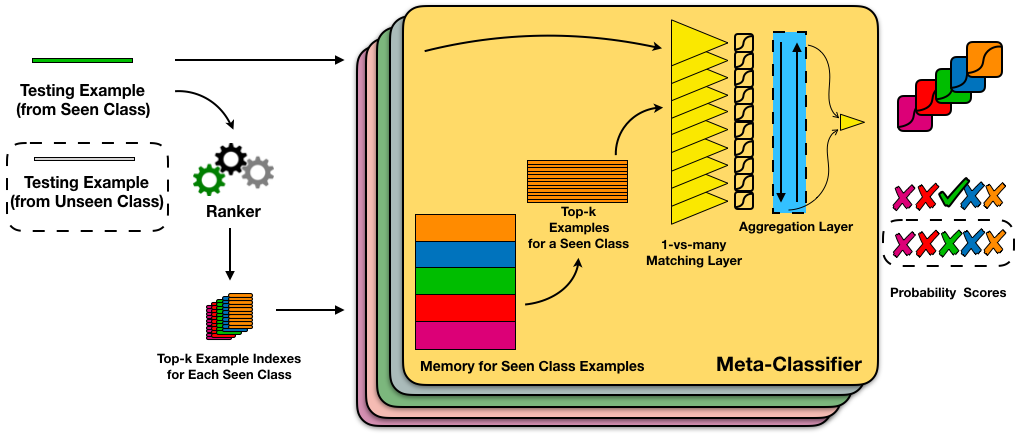
\includegraphics[width=5.5in]{fig/www19_overview.png}
\caption{Overview of the L2AC framework (best viewed in colors). Assume the seen class set $S$ has 5 classes and their examples are indicated by 5 different colors. L2AC has two components: a ranker and a meta-classifier. Given a (green) testing example from a seen class, the ranker first retrieves the top-$k$ nearest examples (memory indexes) from each seen class. Then the meta-classifier takes both the test example and the top-$k$ nearest examples for a seen class to produce a probability score for that class. The meta-classifier is applied 5 times (indicated by 5 rounded rectangles) over these 5 seen classes and yields 5 probability scores, where the 3rd (green) class attends the maximum score as the final class (green) prediction. However, if the test example (grey) is from an unseen class (as indicated by the dashed box), none of those probability scores from the seen classes will predict positive, which leads rejection.}
\label{chap2:fig:overview}
\end{figure*}

%\subsection{Meta-Classifier}
\textbf{Meta-Classifier}
Meta-classifier serves as the core component of the L2AC framework. It is essentially a binary classifier on a given seen class. It takes the top-$k$ nearest examples (to the test example $x_t$) of the seen class as the input and determines whether $x_t$ belongs to that seen class or not.
In this section, we first describe how to represent examples of a seen class. Then we describe how the meta-classifier processes these examples together with the test example into an overall probability score (via a voting mechanism) for deciding whether the test example should belong to any seen class (classification) or not (rejection). Along with that we also describe how a joint decision is made for open-world classification over a set of seen classes. Finally, we describe how to train the meta-classifier via another set of meta-training classes and their examples.

%\subsubsection{Example Representation and Memory}
\textbf{Example Representation and Memory}
\label{chap2:sec:mem}
Representation learning lives at the heart of neural networks. 
Following the success of using pre-trained weights from large-scale image datasets (such as ImageNet \cite{russakovsky2015imagenet}) as feature encoders, we assume there is an encoder that captures almost all features for text classification.

Given an example $x$ representing a text document (a sequence of tokens), we obtain its continuous representation (a vector) via an encoder $h=g(x)$, where the encoder $g(\cdot)$ is typically a neural network (e.g., CNN or LSTM).
We will detail a simple encoder implementation in Sec. \ref{chap2:sec:exp}.

Further, we save the continuous representations of the examples into the memory of the meta-classifier.
So later, the top-$k$ examples can be efficiently retrieved via the index (address) in the memory. 
The memory is essentially a matrix $E \in \mathbb{R} ^{n \times |h|}$, where $n$ is the number of all examples from seen classes and $|h|$ is the size of the hidden dimensions.
Note that we will still use $x$ instead of $h$ to refer to an example for brevity.
Given the test example $x_t$, the meta-classifier first looks up the actual continuous representations $x_{a_{1:k} }$ of the top-$k$ examples for a seen class.
Then the meta-classifier computes the similarity score between $x_t$ and each $x_{a_{i} }$ ($1\le i \le k$) individually via a 1-vs-many matching layer as described next. 

%\subsubsection{1-vs-many Matching Layer}
\textbf{1-vs-many Matching Layer}
\label{chap2:sec:1vsmany}

To compute the overall probability between a test example and a seen class, a 1-vs-many matching layer in the meta-classifier first computes the individual similarity score between the test example and each of the top-$k$ retrieved examples of the seen class. 
The 1-vs-many matching layer essentially consists of $k$ shared matching networks as indicated by big yellow triangles in Fig. \ref{chap2:fig:overview}.
We denote each matching network as $f(\cdot, \cdot)$ and compute similarity scores $r_{1:k}$ for all top-$k$ examples $r_{1:k}=f(x_t, x_{a_{1:k}} )$.

The matching network first transforms the test example $x_t$ and $x_{a_{i}}$ from the continuous representation space to a single example in a similarity space.
We leverage two similarity functions to obtain the similarity space.
The first function is the absolute values of the element-wise subtraction:
$f_\text{abssub}(x_t, x_{a_{i}})=|x_t - x_{a_{i}}|$.
The second one is the element-wise summation:
$f_\text{sum}(x_t, x_{a_{i}})=x_t + x_{a_{i}}$.
Then the final similarity space is the concatenation of these two functions' results:
$f_\text{sim}(x_t, x_{a_{i}})=f_\text{abssub}(x_t, x_{a_{i}}) \oplus f_\text{sum}(x_t, x_{a_{i}})$, where $\oplus$ denotes the concatenation operation.
We then pass the result to two fully-connected layers (one with Relu activation) and a sigmoid function: 
\begin{equation}
\label{chap2:eq:r}
r_i=f(x_t, x_{a_i} )=\sigma\Big(W_2\cdot\text{Relu}\big(W_1\cdot f_\text{sim}(x_t, x_{a_i} ) +b_1\big)+b_2\Big).
\end{equation}
Since there are $k$ nearest examples, we have $k$ similarity scores denoted as $r_{1:k}$.
The hyper-parameters are detailed in Sec. \ref{chap2:sec:exp}.

%\subsubsection{Open-world Learning via Aggregation Layer}
\textbf{Open-world Learning via Aggregation Layer}
\label{chap2:sec:agg}
After getting the individual similarity scores, an aggregation layer in the meta-classifier merges the $k$ similarity scores into a single probability indicating whether the test example $x_t$ belongs to the seen class.
By having the aggregation layer, the meta-classifier essentially has a \textit{parametric voting mechanism} so that it can learn how to vote on multiple nearest examples (rather than a single example) from a seen class to decide the probability.
As a result, the meta-classifier can have more reliable predictions, which is studied in Sec. \ref{chap2:sec:exp}.

We adopt a (many-to-one) BiLSTM \cite{hochreiter1997long,schuster1997bidirectional} as the aggregation layer.
We set the output size of BiLSTM to 2 (1 per direction of LSTM). 
Then the output of BiLSTM is connected to a fully-connected layer followed by a sigmoid function that outputs the probability.
The computation of the meta-classifier for a given test example $x_t$ and $x_{a_{1:k}}$ for a seen class $c$ can be summarized as: 
\begin{equation}
    \label{chap2:eq:p}
p(c|x_t, x_{a_{1:k}} )=\sigma\big(W\cdot \text{BiLSTM}(r_{1:k})+b\big).
\end{equation}
%Lastly,
Inspired by DOC \cite{shu-xu-liu:2017:EMNLP2017}, 
for each class $c \in S$, we evaluate Eq. \ref{chap2:eq:p} as:
\begin{equation} 
    \label{chap2:eq:rej}
        \hat{y} = \left\{
        \begin{array}{c}
        \textit{reject}, \text{ if } \max_{c \in S} p(c|x_t, x_{a_{1:k}} ) \le 0.5 ;\\
        \\
        \argmax_{c \in S} p(c|x_t, x_{a_{1:k}} ) ,\text{ otherwise.}
        \end{array} \right.
    %     }
\end{equation}
If none of existing seen classes $S$ gives a probability above $0.5$, we \emph{reject} $x_t$ as an example from some unseen class.
Note that given a large number of classes, eq. \ref{chap2:eq:rej} can be efficiently implemented in parallel. We leave this to future work.
To make L2AC an easily accessible approach, we use $0.5$ as the threshold naturally and do not introduce an extra hyper-parameter that needs to be artificially tuned.
Note also that as discussed earlier, the seen class set $S$ and its examples can be dynamically maintained (e.g., one can add to or remove from $S$ any class). So the meta-classifier simply performs open-world classification over the current seen class set $S$.

%\subsection{Training of Meta-Classifier}
\textbf{Training of Meta-Classifier}\\
\label{chap2:sec:train}
% (??? I added a reason)
Since the meta-classifier is a general classifier that is supposed to work for any class,
training the meta-classifier $p_\theta(c|x_t, x_{a_{1:k}|x_t, c} )$
requires examples from another set $M$ of classes called \textit{meta-training classes}.

A large $|M|$ is desirable so that meta-training classes have good coverage of features for seen and unseen classes in testing, which is in similar spirit to few-shot learning \cite{lake2011one}. 
We also enforce $ (S\cup U) \cap M=\varnothing$ in Sec. \ref{chap2:sec:exp}, so that all seen and unseen classes are totally unknown to the meta-classifier.

Next, we formulate the meta-training examples from $M$, which consist of a set of pairs 
(with positive and negative labels). 
The first component of a pair is a training document $x_q$ from a class in $M$, and the second component is a sequence of top-$k$ nearest examples also from a class in $M$. 

We assume every example (document) of a class in $M$ can be a training document $x_q$.
Assuming $x_q$ is from class $c \in M$,
a positive training pair is $(x_q, x_{a_{1:k}|x_q, c})$, where $x_{a_{1:k}|x_q, c}$ are top-$k$ examples from class $c$ that are most similar or nearest to $x_q$;
a negative training pair is $(x_q, x_{a_{1:k}|x_q, c'})$, where $c' \in M$, $c \neq c'$ and $x_{a_{1:k}|x_q, c'}$ are top-$k$ examples from class $c'$ that are nearest to $x_q$.
We call $c'$ one \emph{negative class} for $x_q$.
Since there are many negative classes $c' \in M\backslash c$ for $x_q$, we keep top-$n$ negative classes for each training example $x_q$. 
That is, each $x_q$ has one positive training pair and $n$ negative training pairs.
To balance the classes in the training loss, we give a weight ratio $n:1$ for a positive and a negative pair, respectively.

Training the meta-classifier also requires validation classes for model selection (during optimization) and hyper-parameters ($k$ and $n$) tuning (as detailed in Experiments).
Since the classes tested by the meta-classifier are unexpected, we further use a set of  \textit{validation classes} $M'\cap M=\varnothing$ (also $M'\cap (S\cup U)=\varnothing$), to ensure generalization on the seen/unseen classes.

\section{Results}
\label{chap2:sec:exp}

We want to address the following Research Questions (RQs):
\textbf{RQ1} - what is the performance of the meta-classifier with different settings of top-$k$ examples and $n$ negative classes?
\textbf{RQ2} - How is the performance of L2AC compared with state-of-the-art text classifiers for open-world classification (which all need some forms of re-training).

%\subsection{Dataset}
\textbf{Dataset}\\
We leverage the huge amount of product descriptions from the Amazon Datasets \cite{he2016ups} and form the OWL task as the following.
Amazon.com maintains a tree-structured category system. 
We consider each path to a leaf node as a class.
We removed products belonging to multiple classes to ensure the classes have no overlapping.
This gives us 2598 classes, where 1018 classes have more than 400 products per class.
We randomly choose 1000 classes from the 1018 classes with 400 randomly selected products per class as the \textit{encoder training set};
100 classes with 150 products per class are used as the (classification) \textit{test set}, including both seen classes $S$ and unseen classes $U$;
another 1000 classes with 100 products per class are used as the \textit{meta-training set} (including both $M$ and $M'$).
For the 100 classes of the test set, we further hold out 50 examples (products) from each class as test examples. 
The rest 100 examples are training data for baselines, or seen classes examples to be read by the meta-classifier (which only reads those examples but is not trained on those examples).
To train the meta-classifier, we further split the meta-training set as 900 \textit{meta-training classes} ($M$) and 100 \textit{validation classes} ($M'$).
For all datasets, we use NLTK(\url{https://www.nltk.org/}) as the tokenizer, and regard all words that appear more than once as the vocabulary.
This gives us 17,526 unique words.
We take the maximum length of each document as 120 since the majority of product descriptions are under 100 words.

%\subsection{Ranker}
\textbf{Ranker}\\
We use cosine similarity to rank the examples in each seen (or meta-training) class for a given test (or meta-training) example $x_t$ (or $x_q$)(Given many examples to process, the ranker can be implemented in a fully parallel fashion to speed up the processing, which we leave to future work as it is beyond the scope of this work.).
We apply cosine directly on the hidden representations of the encoder as $cosine(h_*, h_{a_{i}})=\frac{h_* \cdot h_{a_{i}}}{|h_*|_2|h_{a_{i}}|_2}$, where $*$ can be either $t$ or $q$, $|\cdot|_2$ denotes the $l$-2 norm and $\cdot$ denotes the dot product of two examples.

Training the meta-classifier also requires a ranking of negative classes for a meta-training example $x_q$, as discussed in Sec. %\ref{sec:train}.
We first compute a \textit{class vector} for each meta-training class. 
This class vector is averaged over all encoded representations of examples of that class.
Then we rank classes by computing cosine similarity between the class vectors and the meta-training example $x_q$.
The top-$n$ (defined in the previous section) classes are selected as negative classes for $x_q$.
We explore different settings of $n$ later.

%\subsection{Evaluation}
\textbf{Evaluation}\\
Similar to \cite{shu-xu-liu:2017:EMNLP2017}, we choose 25, 50, and 75 classes from the (classification) test set of 100 classes as the seen classes for three (3) experiments.
Note that each class in the test set has 150 examples, where 100 examples are for the training of baseline methods or used as seen class examples for L2AC and 50 examples are for testing both the baselines and L2AC.
We evaluate the results on all 100 classes for those three (3) experiments.
For example, when there are 25 seen classes, testing examples from the rest 75 unseen classes are taken as from one \textit{rejection class} $c_\text{rej}$, as in \cite{shu-xu-liu:2017:EMNLP2017}.

Besides using macro F1 as used in \cite{shu-xu-liu:2017:EMNLP2017}, we also use weighted F1 score overall classes (including seen and the rejection class) as the evaluation metric.
Weighted F1 is computed as 
\begin{equation}
\sum_{c\in S\cup\{c_\text{rej}\} } \frac{N_c}{\sum_{c\in S\cup\{c_\text{rej}\}}N_c  }\cdot \text{F1}_c,
\end{equation}
where $N_c$ is the number of examples for class $c$ and $\text{F1}_c$ is the F1 score of that class.
We use this metric because macro F1 has a bias on the importance of rejection when the seen class set is small (macro F1 treats the rejection class as equally important as one seen class).
For example, when the number of seen classes is small, the rejection class should have a higher weight as a classifier on a small seen set is more likely challenged by examples from unseen classes.
Further, to stabilize the results, we train all models with 10 different initializations and average the results.

%\subsection{Hyper-parameters}
\textbf{Hyper-parameters}\\
For simplicity, we leverage a BiLSTM \cite{hochreiter1997long,schuster1997bidirectional} on top of a GloVe \cite{pennington2014glove} embedding (840b.300d) layer as the encoder (other choices are also possible).
Similar to feature encoders trained from ImageNet~\cite{russakovsky2015imagenet}, we train classification over the encoder training set with 1000 classes and use 5\% of the encoding training data as encoder validation data.
We apply dropout rates of 0.5 to all layers of the encoder. 
The classification accuracy of the encoder on validation data is \textbf{81.76\%}.
The matching network (the shared network within the 1-vs-many matching layer) has two fully-connected layers, where the size of the hidden dimension is 512 with a dropout rate of 0.5.
We set the batch size of meta-training as 256.

To answer RQ1 on two hyper-parameters $k$ (number of nearest examples from each class) and $n$ (number of negative classes), we use the 100 validation classes to determine these two hyper-parameters.
We formulate the validation data similar to the testing experiment on 50 seen classes.
For each validation class, we select 50 examples for validation. The rest 50 examples from each validation seen class are used to find top-$k$ nearest examples.
We perform grid search of averaged weighted F1 over 10 runs for $k\in\{1, 3, 5, 10, 15, 20\}$ and $n\in \{1, 3, 5, 9\}$, where \textbf{$k=5$} and \textbf{$n=9$} reach a reasonably well weighted F1 (87.60\%). Further increasing $n$ gives limited improvements (e.g., 87.69\% for $n=14$ and 87.68\% for $n=19$, when $k=5$). But a large $n$ significantly increases the number of training examples (e.g., $n=14$ ended with more than 1 million meta-training examples) and thus training time. So we decide to select $k=5$ and $n=9$ for all ablation studies below.
Note the validation classes are also used to compute (formulated in a way similar to the meta-training classes) the validation loss for selecting the best model during Adam \cite{kingma2014adam} optimization.

%\subsection{Compared Methods}
\textbf{Compared Methods}\\

\begin{table*}[t]
\centering    
\scalebox{0.95}{

\begin{tabular}{l||c|c|c|c|c|c}
\hline
{\bf Methods} & $|S|=25$ (WF1) & $|S|=25$ (MF1) & $|S|=50$ (WF1) & $|S|=50$ (MF1) & $|S|=75$ (WF1) & $|S|=75$ (MF1) \\
\hline
DOC-CNN & 53.25(1.0) & 55.04(0.39) & 70.57(0.46) & 76.91(0.27) & 81.16(0.47) & 86.96(0.2) \\
DOC-LSTM & 57.87(1.26) & 57.6(1.18) & 69.49(1.58) & 75.68(0.78) & 77.74(0.48) & 84.48(0.33) \\
DOC-Enc & 82.92(0.37) & 75.09(0.33) & 82.53(0.25) & 84.34(0.23) & 83.84(0.36) & 88.33(0.19) \\
\hline
DOC-CNN-Gaus & 85.72(0.43) & 76.79(0.41) & 83.33(0.31) & 83.75(0.26) & 84.21(0.12) & 87.86(0.21) \\
DOC-LSTM-Gaus & 80.31(1.73) & 70.49(1.55) & 77.49(0.74) & 79.45(0.59) & 80.65(0.51) & 85.46(0.25) \\
DOC-Enc-Gaus & 88.54(0.22) & 80.77(0.22) & 84.75(0.21) & 85.26(0.2) & 83.85(0.37) & 87.92(0.22) \\
\hline
\hline
L2AC-$n$9-NoVote & 91.1(0.17) & 82.51(0.39) & 84.91(0.16) & 83.71(0.29) & 81.41(0.54) & 85.03(0.62) \\
L2AC-$n$9-Vote3 & 91.54(0.55) & 82.42(1.29) & 84.57(0.61) & 82.7(0.95) & 80.18(1.03) & 83.52(1.14) \\
\hline
L2AC-$k$5-$n$9-AbsSub & 92.37(0.28) & 84.8(0.54) & 85.61(0.36) & 84.54(0.42) & 83.18(0.38) & 86.38(0.36) \\
L2AC-$k$5-$n$9-Sum & 83.95(0.52) & 70.85(0.91) & 76.09(0.36) & 75.25(0.42) & 74.12(0.51) & 78.75(0.57) \\
\hline
L2AC-$k$\textbf{5}-$n$\textbf{9} & \underline{93.07}(0.33) & 86.48(0.54) & \underline{86.5}(0.46) & 85.99(0.33) & \underline{84.68}(0.27) & 88.05(0.18) \\
L2AC-$k$5-$n$14 & \textbf{93.19}(0.19) & 86.91(0.33) & \textbf{86.63}(0.28) & 86.42(0.2) & 85.32(0.35) & 88.72(0.23) \\
L2AC-$k$5-$n$19 & 93.15(0.24) & 86.9(0.45) & 86.62(0.49) & 86.48(0.43) & \textbf{85.36}(0.66) & 88.79(0.52) \\
\hline
\end{tabular}
    }
\caption{Weighted F1 (WF1) and macro F1 (MF1) scores on a test set with 100 classes with 3 settings: 25, 50, and 75 seen classes. The set of seen classes are incrementally expanded from 25 to 75 classes (or gradually shrunk from 75 to 25 classes). The results are the averages over 10 runs with standard deviations in parenthesis.}
 \vspace{-3mm}
\label{chap2:tbl:result}
\end{table*}

\begin{figure}    
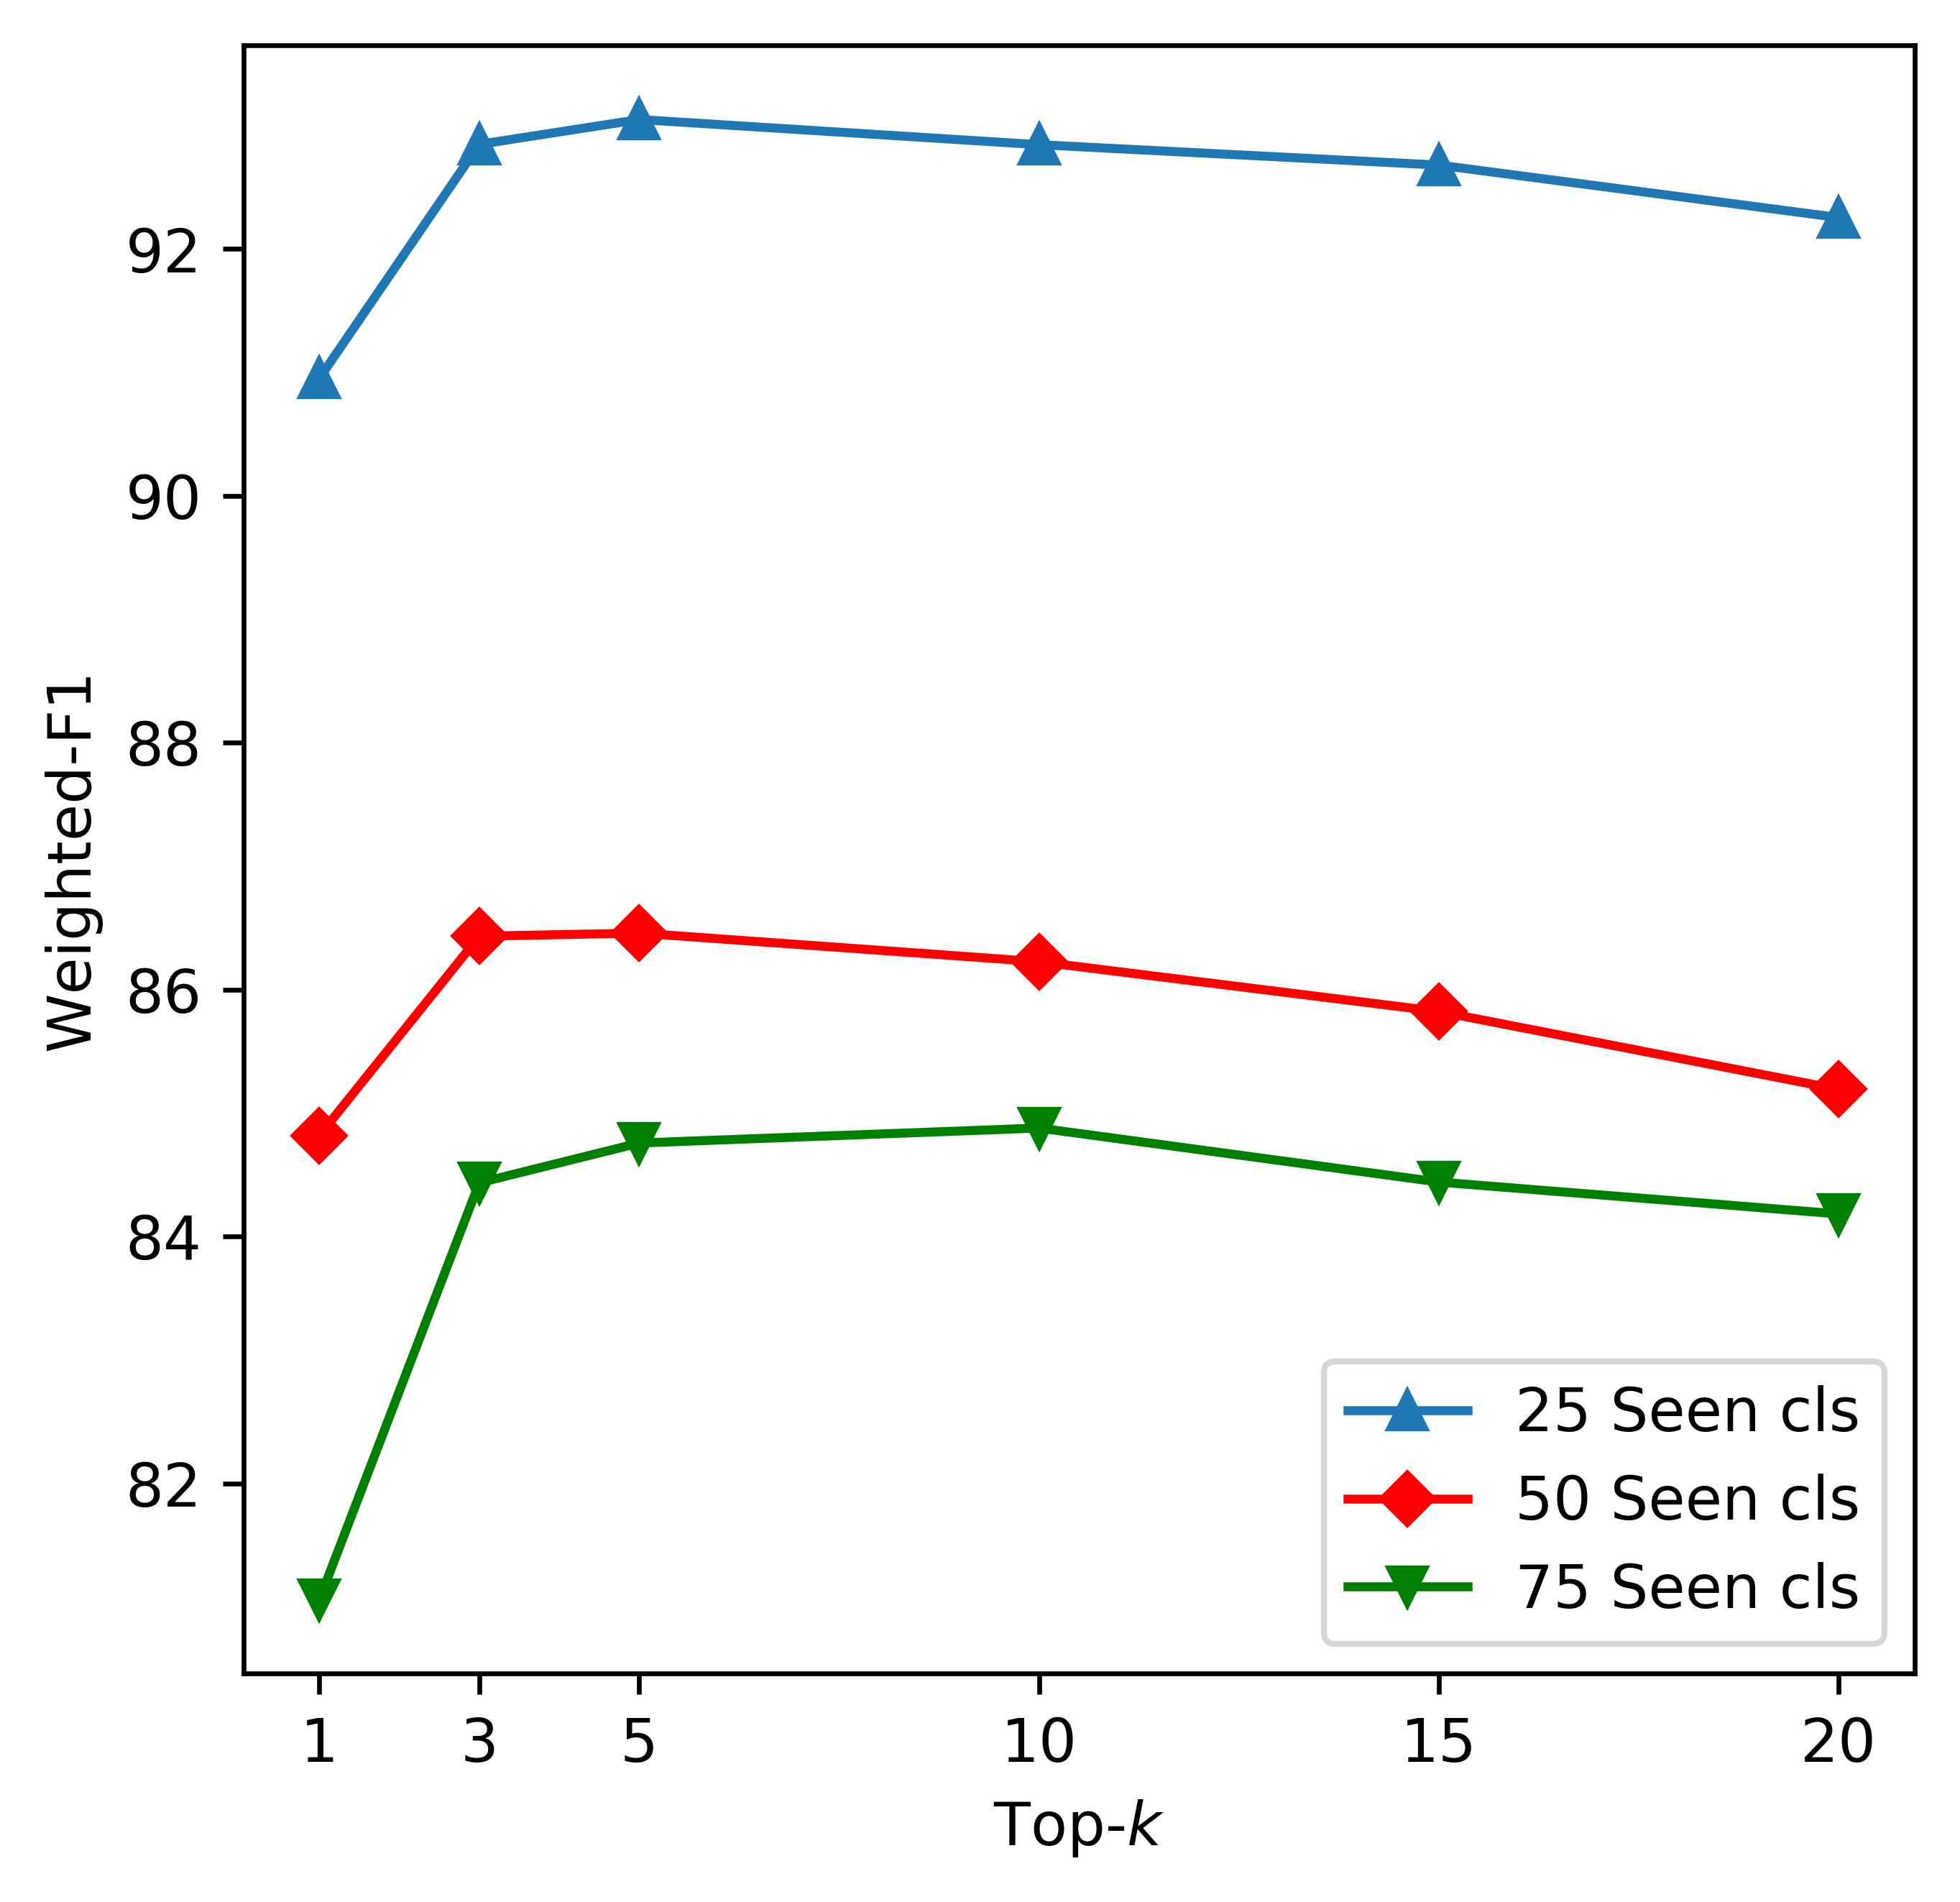
\includegraphics[width=1.55in]{fig/www19_top_k.png}
\quad
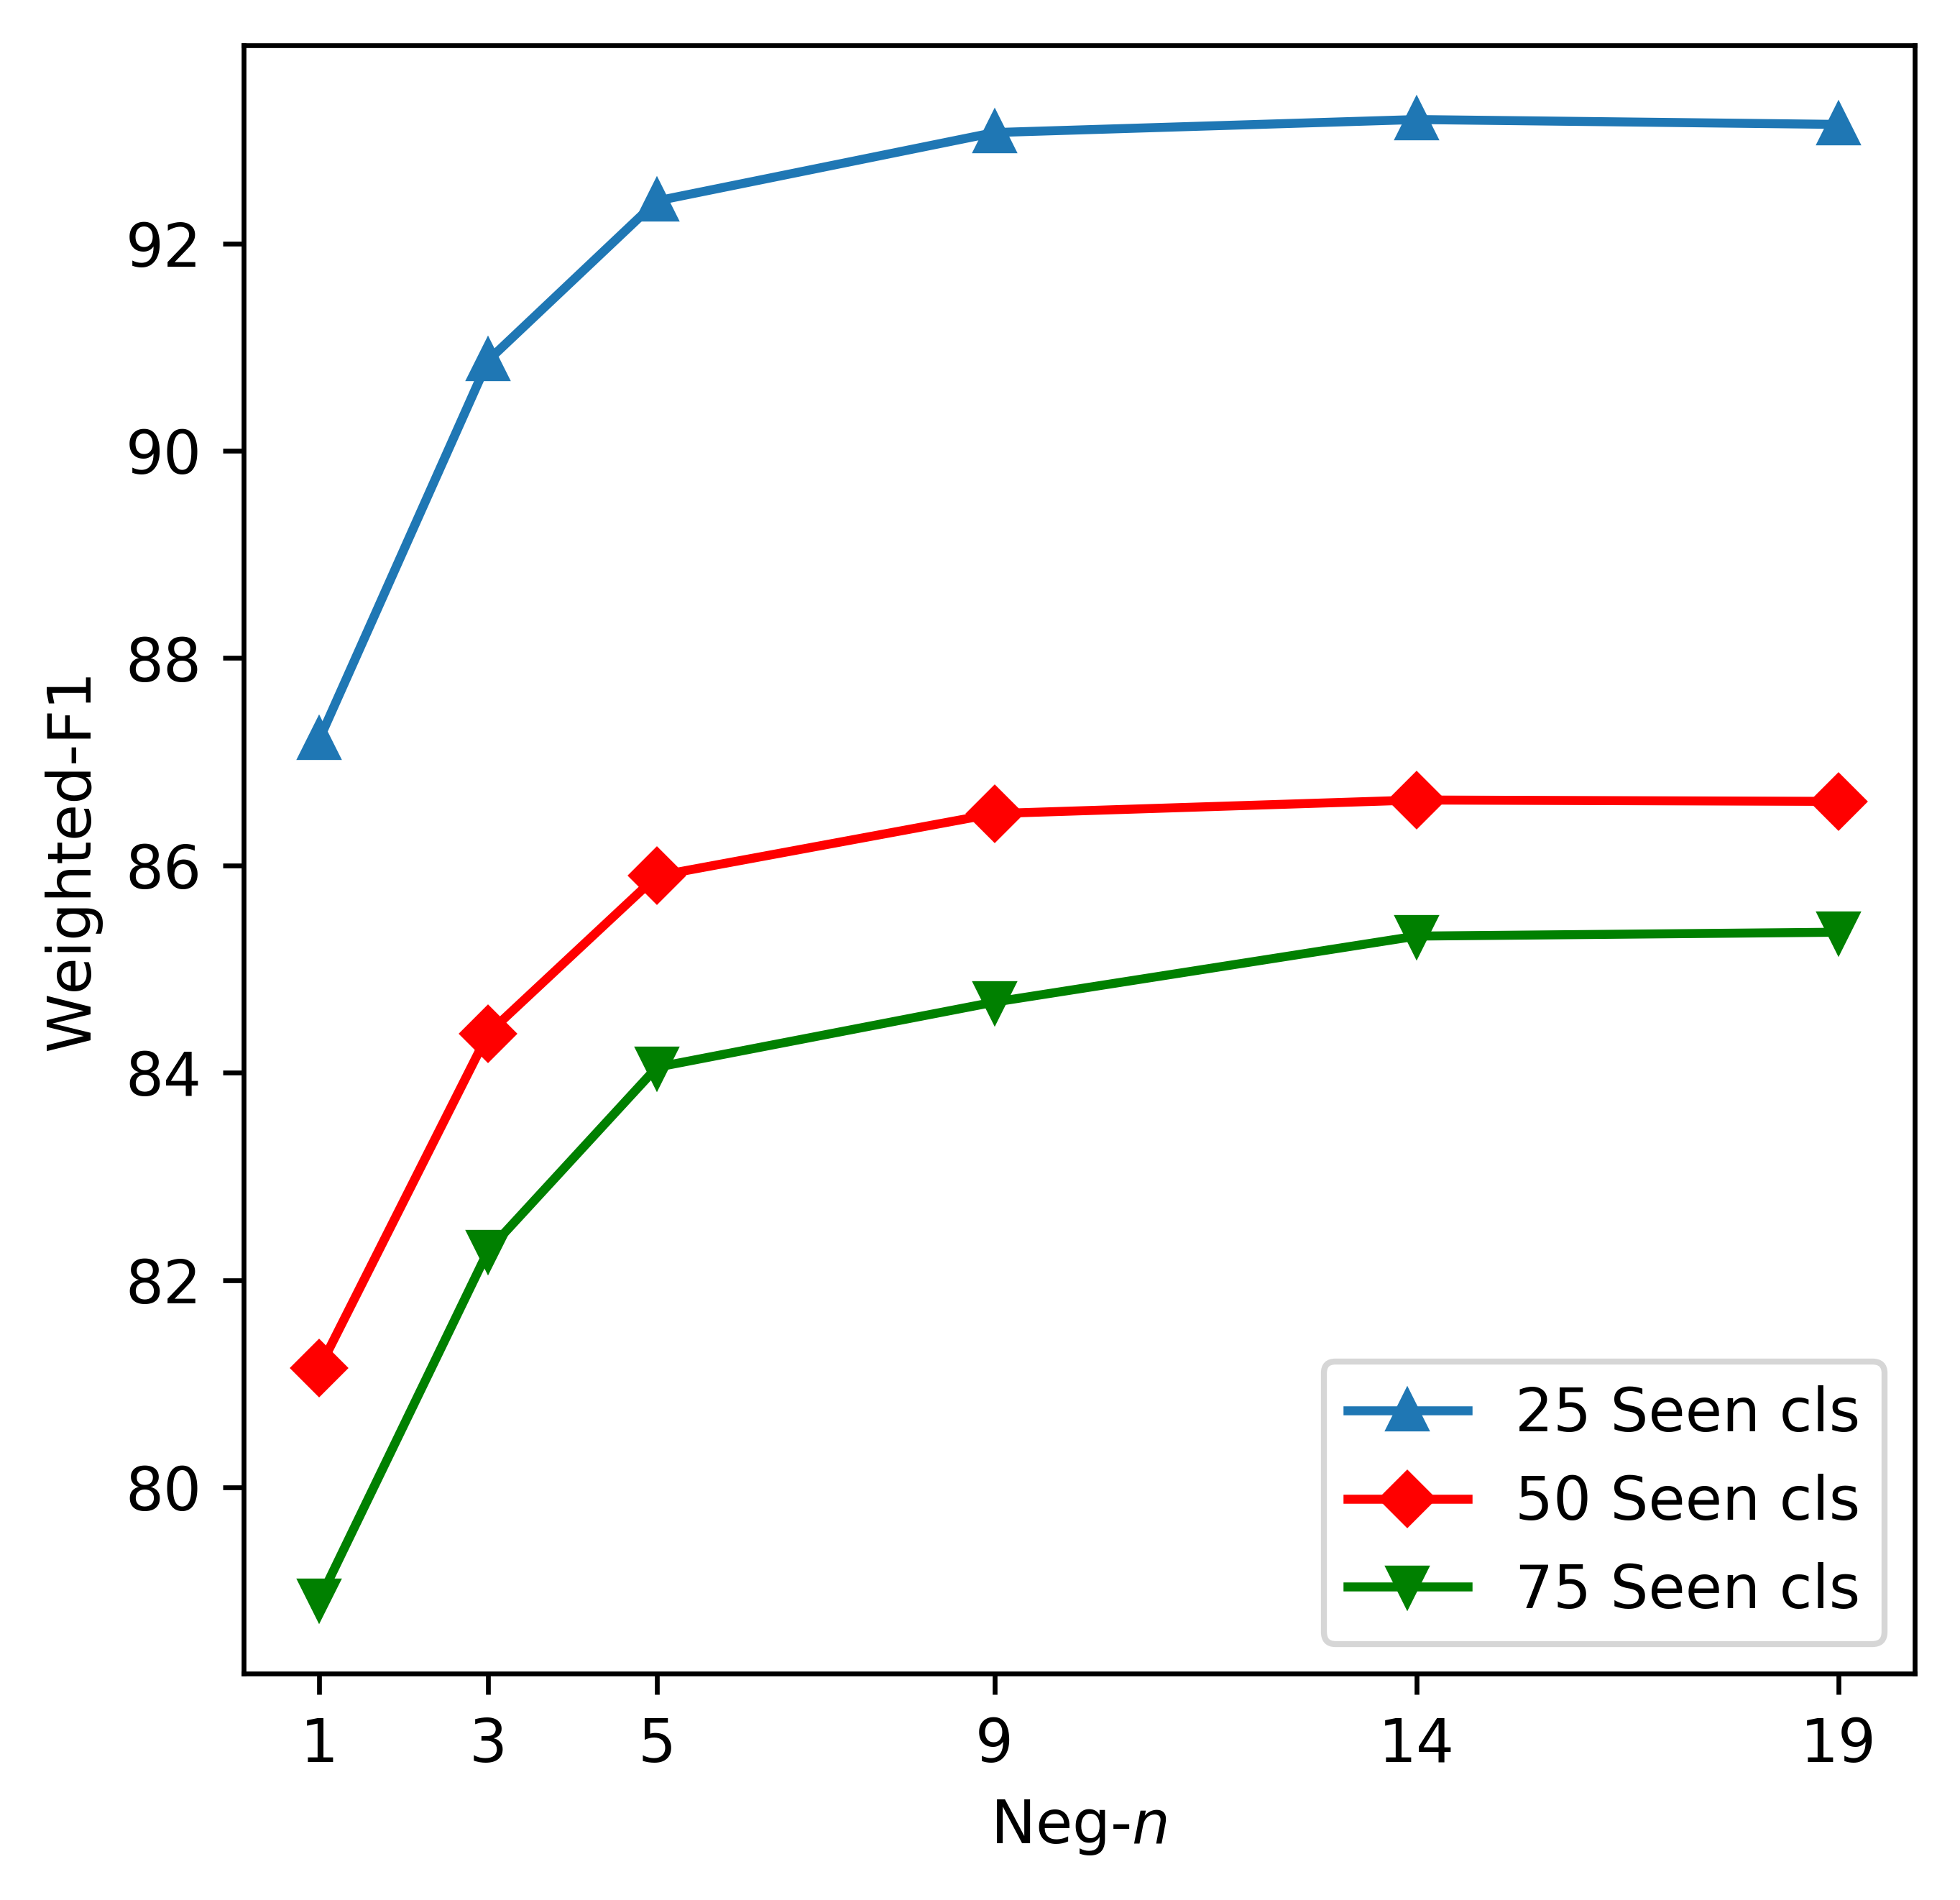
\includegraphics[width=1.55in]{fig/www19_neg_n.png}
\caption{Weighted F1 scores for different $k$'s ($n=9$) and different $n$'s ($k=5$).}
\label{chap2:fig:kn}
\end{figure}

To the best of our knowledge, DOC \cite{shu-xu-liu:2017:EMNLP2017} is the only state-of-the-art baseline for open-world learning (with rejection) for text classification. It has been shown in \cite{shu-xu-liu:2017:EMNLP2017} that DOC significantly outperforms the methods CL-cbsSVM and cbsSVM in~\cite{fei2016learning} and OpenMax in~\cite{bendale2016towards}. OpenMax is a state-of-the-art method for image classification with rejection capability. 
To answer RQ2, we use DOC and its variants to show that the proposed method has comparable performance with the best open-world learning method with re-training.
Note that DOC cannot incrementally add new classes. 
So we re-train DOC over different sets of seen classes from scratch every time new classes are added to that set.

It is thus actually unfair to compare our method with DOC because DOC is trained on the actual training examples of all classes. However, our method still performs better in general. We used the original code of DOC and created six (6) variants of it.

\vspace{+2mm}
\noindent
\textbf{DOC-CNN}: CNN implementation as in the original DOC paper without Gaussian fitting (using 0.5 as the threshold for rejection). It operates directly on a sequence of tokens. \\
\textbf{DOC-LSTM}: a variant of DOC-CNN, where we replace CNN with BiLSTM to encode the input sequence for fair comparison. BiLSTM is trainable and the input is still a sequence of tokens. \\
\textbf{DOC-Enc}: this is adapted from DOC-CNN, where we remove the feature learning part of DOC-CNN and feed the hidden representation from our encoder directly to the fully-connected layers of DOC for a fair comparison with L2AC. \\
\textbf{DOC-*-Gaus}: applying Gaussian fitting proposed in \cite{shu-xu-liu:2017:EMNLP2017} on the above three baselines, we have 3 more DOC baselines. 
Note that these 3 baselines have exactly the same models as above respectively. They only differ in the thresholds used for rejection. Gaussian fitting in \cite{shu-xu-liu:2017:EMNLP2017} is used to set a good threshold for rejection. 
We use these baselines to show that the Gaussian fitted threshold improves the rejection performance of DOC significantly but may lower the performance of seen class classification. The original DOC is \textbf{DOC-CNN-Gaus} here. 

\vspace{+1mm}
The following baselines are variants of L2AC.\\
\textbf{L2AC-$n$9-NoVote}: this is a variant of the proposed L2AC that only takes one most similar example (from each class), i.e., $k=1$, with one positive class paired with $n=9$ negative classes in meta-training ($n=9$ has the best performance as indicated in answering RQ1 above). 
We use this baseline to show that the performance of taking only one sample may not be good enough.
This baseline clearly does not have/need the aggregation layer and only has a single matching network in the 1-vs-many layer.\\
\textbf{L2AC-$n$9-Vote3}: this baseline uses exactly the same model as L2AC-$n$9-NoVote. But during evaluation, we allow a non-parametric voting process (like $k$NN) for prediction. We report the results of voting over top-3 examples per seen class as it has the best result (ranging from 3 to 10). If the average of the top-3 similar examples in a seen class has example scores with more than $0.5$, L2AC believes the testing example belongs to that class.
We use this baseline to show that the aggregation layer is effective in learning to vote and L2AC can use more similar examples and get better performance.\\

\textbf{L2AC-$k$5-$n$9-AbsSub/Sum}: To show that using two similarity functions ($f_\text{abssub}(\cdot, \cdot)$ and $f_\text{sum}(\cdot, \cdot)$ ) gives better results, we further perform ablation study by using only one of those similarity functions at a time, which gives us two baselines.\\
\textbf{L2AC-$k$5-$n$9/14/19}: this baseline has the best $k=5$ and $n=9$ on the validation classes, as indicated in the previous subsection. Interestingly, further increasing $k$ may reduce the performance as L2AC may focus on not-so-similar examples. We also report results on $n=14$ or $19$ to show that the results do not get much better. 

%\subsection{Results Analysis}
\textbf{Results Analysis}\\
From Table \ref{chap2:tbl:result}, we can see that L2AC outperforms DOC, especially when the number of seen classes is small. 
First, from Fig. \ref{chap2:fig:kn} we can see that $k=5$ and $n=9$ gets reasonably good results.
Increasing $k$ may harm the performance as taking in more examples from a class may let L2AC focus on not-so-similar examples, which is bad for classification. More negative classes give L2AC better performance in general but further increasing $n$ beyond 9 has little impact.

Next, we can see that as we incrementally add more classes, L2AC gradually drops its performance (which is reasonable due to more classes) but it still yields better performance than DOC. Considering that L2AC needs no training with additional classes, while DOC needs full training from scratch, L2AC  represents a major advance. Note that testing on 25 seen classes is more about testing a model's rejection capability while testing on 75 seen classes is more about the classification performance of seen class examples.
From Table \ref{chap2:tbl:result}, we notice that L2AC can effectively leverage multiple nearest examples and negative classes.
In contrast, the non-parametric voting of L2AC-$n$9-Vote3 over top-3 examples may not improve the performance but introduce higher variances.
Our best $k=5$ indicates that the meta-classifier can dynamically leverage multiple nearest examples instead of solely relying on a single example.
As an ablation study on the choices of similarity functions, running L2AC on a single similarity function gives poorer results as indicated by either L2AC-$k$5-$n$9-AbsSub or L2AC-$k$5-$n$9-Sum.

DOC without encoder (DOC-CNN or DOC-LSTM) performs poorly when the number of seen classes is small.
Without Gaussian fitting, DOC's (DOC-CNN, DOC-LSTM or DOC-Enc) performance increases as more classes are added as seen classes. This is reasonable as DOC is more challenged by fewer seen training classes and more unseen classes during testing. 
As such, Gaussian fitting (DOC-*-Gaus) alleviates the weakness of DOC on a small number of seen training classes.


\chapter{Lifelong Word Representation Learning}
\label{chap3:word}

Learning word embeddings \cite{mnih2007three,mikolov2013efficient,mikolov2013distributed,pennington2014glove}
has received a great deal of attention due to its success in numerous NLP applications, e.g., named entity recognition \cite{sienvcnik2015adapting}, sentiment analysis \cite{maas2011learning} and syntactic parsing \cite{durrett2015neural}.
The key to the success of word embeddings is that a large-scale corpus can be turned into a huge number (e.g., billions) of training examples.

Two implicit assumptions are often made about the effectiveness of embeddings to down-stream tasks: 
1) the training corpus for embedding is available and much larger than the training data of the down-stream task; 2) the topic (domain) of the embedding corpus is closely aligned with the topic of the down-stream task.
However, many real-life applications do not meet both assumptions.

In most cases, the in-domain corpus is of limited size, which is insufficient for training good embeddings. 
In applications, researchers and practitioners often simply use some general-purpose embeddings trained using a very large general-purpose corpus (which satisfies the first assumption) covering almost all possible topics, e.g., the  GloVe embeddings \cite{pennington2014glove} trained using 840 billion tokens covering almost all topics/domains on the Web. Such embeddings have been shown to work reasonably well in many domain-specific tasks. This is not surprising as the meanings of a word are largely shared across domains and tasks. However, this solution violates the second assumption, which often leads to sub-optimal results for domain-specific tasks, as shown in our experiments.
One obvious explanation for this is that the general-purpose embeddings do provide some useful information for many words in the domain task, but their embedding representations may not be ideal for the domain and in some cases they may even conflict with the meanings of the words in the task domain because words often have multiple senses or meanings.
For example, we have a task in the programming domain, which has the word ``Java''. A large-scale general-purpose corpus, which is very likely to include texts about coffee shops, supermarkets, the Java island of Indonesia, etc., can easily squeeze the room for representing ``Java''' context words like ``function'', ``variable'' or ``Python'' in the programming domain.
This results in a poor representation of the word ``Java'' for the programming task.  

\section{Motivation}
\label{chap3:sec:intro}

Thus, learning high-quality domain word embeddings is important for achieving good performance in many NLP tasks. General-purpose embeddings trained on large-scale corpora are often sub-optimal for domain-specific applications. However, domain-specific tasks often do not have large in-domain corpora for training high-quality domain embeddings.

As such, we propose a novel \textit{lifelong learning} setting for domain embedding. That is, when performing the new domain embedding, the system has seen many past domains, and it tries to expand the new in-domain corpus by exploiting the corpora from the past domains via meta-learning. The proposed meta-learner characterizes the similarities of the contexts of the same word in many domain corpora, which helps retrieve relevant data from the past domains to expand the new domain corpus. 

To solve this problem and also the limited in-domain corpus size problem, cross-domain embeddings have been investigated \cite{bollegala-maehara-kawarabayashi:2015:ACL-IJCNLP,yang-lu-zheng:2017:EMNLP2017,bollegala2017think} via transfer learning \cite{pan2010survey}.
These methods allow some in-domain words to leverage the general-purpose embeddings in the hope that the meanings of these words in the general-purpose embeddings do not deviate much from the in-domain meanings of these words. The embeddings of these words can thus be improved. However, these methods cannot improve the embeddings of many other words with domain-specific meanings (e.g., ``Java'').
Further, some words in the general-purpose embeddings may carry meanings that are different from those in the task domain. 

\section{Lifelong Domain Word Embeddings}

As a result, we propose a novel direction for domain embedding learning by expanding the in-domain corpus. The problem in this new direction can be stated as follows:

\textbf{Problem statement}: We assume that the learning system has seen $n$ domain corpora in the past: $D_{1:n}=\{D_1, \dots, D_n\}$, when a new domain corpus $D_{n+1}$ comes with a certain task, the system automatically generates word embeddings for the $(n+1)$-th domain by leveraging some useful information or knowledge from the past $n$ domains.

This problem definition is in the
\textit{lifelong learning} (LL) setting, where the new or $(n+1)$-th task is performed with the help of the knowledge accumulated over the past $n$ tasks \cite{ChenLiu2016}. 
%Silver2013
Clearly, the problem does not have to be defined this way with the domains corpora coming in a sequential manner. It will still work as long as we have $n$ existing domain corpora and we can use them to help with our target domain embedding learning, i.e., the $(n+1)$-th domain.

The main challenges of this problem are 2-fold:
1) how to automatically identify relevant information from the past $n$ domains with no user help, and 2) how to integrate the relevant information into the $(n+1)$-th domain corpus. We propose a meta-learning based system L-DEM (\underline{L}ifelong \underline{D}omain \underline{E}mbedding via \underline{M}eta-learning) to tackle the challenges.

To deal with the first challenge, for a word in the new domain, L-DEM learns to identify similar contexts of the word in the past domains. Here the context of a word means the surrounding words of that word in a domain corpus. We call such context \emph{domain context} (of a word). For this, we introduce a multi-domain meta-learner that can identify similar (or relevant) domain contexts that can be later used in embedding learning in the new domain. To tackle the second challenge, L-DEM augments the new domain corpus with the relevant domain contexts (knowledge) produced by the meta-learner from the past domain corpora and uses the combined data to train the embeddings in the new domain. For example. for word ``Java'' in the programming domain (the new domain), the meta-learner will produce similar domain contexts from some previous domains like programming language, software engineering, operating systems, etc. These domain contexts will be combined with the new domain corpus for ``Java" to train the new domain embeddings.

%\section{Related Works}
\textbf{Related Works}\\
\label{chap3:rw}
Learning word embeddings has been studied for a long time \cite{mnih2007three}. 
Many earlier methods used complex neural networks \cite{mikolov2013linguistic}.
More recently, a simple and effective unsupervised model called skip-gram (or word2vec in general) \cite{mikolov2013distributed,mikolov2013linguistic} was proposed to turn a plain text corpus into large-scale training examples without any human annotation.
It uses the current word to predict the surrounding words in a context window.
The learned weights for each word are the embedding of that word.
Although some embeddings trained using large scale corpora are available \cite{pennington2014glove,bojanowski2016enriching}, they are often sub-optimal for domain-specific tasks \cite{bollegala-maehara-kawarabayashi:2015:ACL-IJCNLP,yang-lu-zheng:2017:EMNLP2017,xu:Short,Xu2018pro}. 
However, a single domain corpus is often too small for training high-quality embeddings \cite{Xu2018pro}.

Our problem setting is related to \textit{Lifelong Learning} (LL). Much of the work on LL focused on supervised learning \cite{Thrun1996learning,Silver2013,ChenLiu2016}.
In recent years, several LL works have also been done for unsupervised learning, e.g., topic modeling \cite{chen2014topic}, information extraction \cite{Mitchell2015} and graph labeling \cite{shu2016lifelong}. 
However, we are not aware of any existing research on using LL for word embedding. Our method is based on meta-learning, which is very different from existing LL methods.
Our work is related to transfer learning and multi-task learning \cite{pan2010survey}. Transfer learning has been used in cross-domain word embeddings \cite{bollegala-maehara-kawarabayashi:2015:ACL-IJCNLP,yang-lu-zheng:2017:EMNLP2017}. However, LL is different from transfer learning or multi-task learning \cite{ChenLiu2016}. 
Transfer learning mainly transfers common word embeddings from general-purpose embeddings to a specific domain. We expand the in-domain corpus with similar past domain contexts identified via meta-learning. 

To expand the in-domain corpus, a good measure of the similarity of domain contexts of the same word from two different domains is needed.
We use meta-learning \cite{thrun2012learning} to learn such similarities.
Recently, meta-learning has been applied to various aspects of machine learning, 
such as learning an optimizer \cite{andrychowicz2016learning},
and learning initial weights for few-shot learning \cite{finn2017model}.
The way we use meta-learning is about domain independent learning \cite{JMLR:v17:15-239}. It learns similarities of domain contexts of the same word.

\section{L-DEM Approach}
\label{chap3:sec:ldem}
The proposed L-DEM system is depicted in Figure \ref{chap3:fig:fr}.
Given a series of past domain corpora $D_{1:n}=\{D_1, D_2, \dots, D_n\}$, and a new domain corpus $D_{n+1}$, the system learns to generate the new domain embeddings by exploiting the relevant information or knowledge from the past $n$ domains.
Firstly, a base meta-learner $M$ is trained from the first $m$ past domains (not shown in the figure) (see Section 4), which is later used to predict the similarities of \emph{domain contexts} of the same words from two different domains.
Secondly, assuming the system has seen $n-m$ past domain corpora $D_{m+1:n}$, when a new domain $D_{n+1}$ comes, the system produces the embeddings of the $(n+1)$-th domain as follows (discussed in Section 5):
(i) the base meta-learner first is adapted to the $(n+1)$-th domain as $M_{n+1}$ (not shown in the figure) using the $(n+1)$-th domain corpus;
(ii) for each word $w_{i}$ in the new domain, the system uses the adapted meta-learner $M_{n+1}$ to identify every past domain $j$ that has the word $w_{i}$ with domain context similar to $w_{i}$'s domain context in the new domain (we simply call such domain context from a past domain \emph{similar domain context});
(iii) all new domain words' similar domain contexts from all past domain corpora $D_{m+1:n}$ are aggregated. This combined set is called the \textit{relevant past knowledge} and denoted by $\mathcal{A}$;
(iv) a modified word2vec model that can take both domain corpus $D_{n+1}$ and the relevant past knowledge of $\mathcal{A}$ is applied to produce the embeddings for the $(n+1)$-th new domain.
Clearly, the meta-learner here plays a central role in identifying relevant knowledge from past domains.
We propose a pairwise model as the meta-learner. 

To enable the above operations, we need a knowledge base (KB), which retains the information or knowledge obtained from the past domains. Once the $(n+1)$-th domain embedding is done, its information is also saved in the KB for future use. We discuss the detailed KB content in Section 5.1.
\begin{figure}[t]
    \label{fig:ll}
    \centering    
    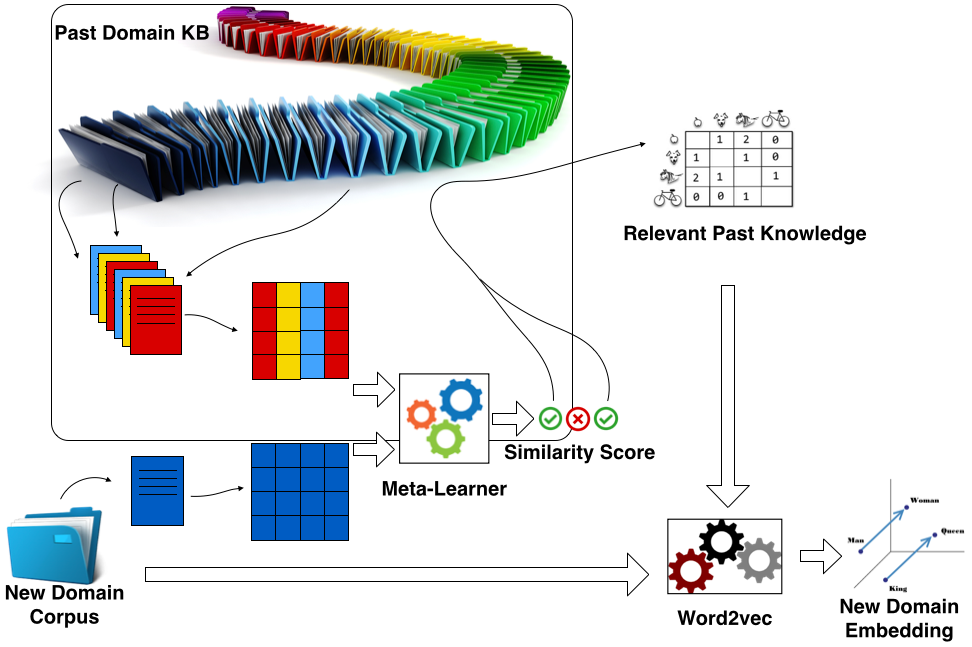
\includegraphics[width=3.3in]{fig/ijcai18_ll.png}
        \caption{Overview of L-DEM.}
        \label{fig:fr}
    \end{figure}

%\section{Base Meta-Learner}
\textbf{Base Meta-Learner}\\
This section describes the base meta-learner, which identifies similar domain contexts. The input to the meta-learner is a pair of word feature vectors (we simply call them \emph{feature vectors}) representing the domain contexts of the same word from two similar / non-similar domains.
The output of the meta-learner is a similarity score of the two feature vectors.

%\subsection{Training Examples}
\textbf{Training Examples}\\
We assume the number of past domains is large and we hold out the first $m$ domains, where $m \ll n$, as the domains to train and test the base meta-learner.
In practice, if $n$ is small, the $m$ domains can be sampled from the $n$ domains.
The $m$ domains are split into 3 disjoint sets: training domains, validation domains, and testing domains.

To enable the meta-learner to predict the similarity score, we need both positive examples (from similar domains) and negative examples (from dissimilar domains).
Since each past domain can be unique (which makes it impossible to have a positive pair from two similar domains), we sub-sample each domain corpus $D_j$ into 2 sub-corpora: $D_{j, k} \sim P(D_i)$, where $1\le j\le m$ and $k=\{1, 2\}$.
This sampling process is done by drawing documents (each domain corpus is a set of documents) uniformly at random from $D_j$.
The number of documents that a domain sub-corpus can have is determined by a pre-defined sub-corpus (file) size (explained in Section 6).
We enforce the same file size across all sub-corpora so feature vectors from different sub-corpora are comparable.

Next, we produce feature vectors from domain sub-corpora.
Given a word $w_{i, j, k}$ (instance of the word $w_{i}$ in the domain sub-corpus $D_{j, k}$), we choose its co-occurrence counts on a fixed vocabulary $V_{\textit{wf}}$ within a context window (similar to word2vec) as the word $w_{i, j, k}$'s feature vector $\mathbf{x}_{w_{i, j, k}}$.
The fixed vocabulary $V_{\textit{wf}}$ (part of the KB used later, denoted as $\mathcal{K}.V_{\textit{wf}}$) is formed from the top-$f$ frequent words over $m$ domain corpora.
This is inspired by the fact that an easy-to-read dictionary (e.g., Longman dictionary) uses only a few thousand words to explain all words of a language.
A pair of feature vectors $(\mathbf{x}_{w_{i, j, k}}, \mathbf{x}_{w_{i, j, k'}})$ with $k \neq k'$, forms a postive example; 
whereas $(\mathbf{x}_{w_{i, j, k}}, \mathbf{x}_{w_{i, j', k}})$ with $j\neq j'$ forms a negative example.
Details of settings are in Section 6.

%\subsection{Pairwise Model of the Meta-learner}
\textbf{Pairwise Model of the Meta-learner}\\
We train a small but efficient pairwise model (meta-learner) to learn similarity score. 
Making the model small but high-throughput is crucial.
This is because the meta-learner is required in a high-throughput inference setting, where every word from a new domain needs to have context similarities with the same word from all past domains. 

The proposed pairwise model has only four layers. 
One shared fully-connected layer (with $l_1$-norm) is used to learn two continuous representations from two (discrete) input feature vectors.
A matching function is used to compute the representation of distance in a high-dimentional space.
Lastly, a fully-connected layer and a sigmoid layer are used to produce the similarity score.
The model is parameterized as follows:
\begin{equation}
\sigma \big( \bm{W}_2 \cdot \text{abs}\big( ( \bm{W}_1 \cdot \frac{\mathbf{x}_{w_{i, j, k}}}{ |\mathbf{x}_{w_{i, j, k}}|_1 }) - (\bm{W}_1 \cdot \frac{\mathbf{x}_{w_{i, j', k'}} }{ |\mathbf{x}_{w_{i, j', k'}}|_1 } ) \big) + b_2 \big) ,
\end{equation}
where $|\cdot|_1$ is the $l_1$-norm, $\text{abs}(\cdot)$ computes the absolute value of element-wise subtraction ($-$) as the matching function, $\bm{W}$s and $b$ are weights and $\sigma (\cdot)$ is the sigmoid function.
The majority of trainable weights resides in $\bm{W}_1$, which learns continuous features from the set of $f$ context words.
These weights can also be interpreted as a general embedding matrix over $V_{\textit{wf}}$. 
These embeddings (not related to the final domain embeddings in Section \ref{chap3:sec:aet}) help to learn the representation of domain-specific words.
As mentioned earlier, we train the base meta-learner $M$ over a hold-out set of $m$ domains.
We further fine-tune the base meta-learner using the new domain corpus for its domain use, as described in the next section.

%\section{Embedding Using Past Relevant Knowledge}
\textbf{Embedding Using Past Relevant Knowledge}
We now describe how to leverage the base meta-learner $M$, the rest $n-m$ past domain corpora, and the new domain corpus $D_{n+1}$ to produce the new domain embeddings.

%\subsection{Identifying Context Words from the Past}
\textbf{Identifying Context Words from the Past}\\
When it comes to borrowing relevant knowledge from past domains, the first problem is what to borrow.
It is well-known that the embedding vector quality for a given word is determined by the quality and richness of that word's contexts.
We call a word in a domain context of a given word a \emph{context word}.
So for each word in the new domain corpus, we should borrow all context words from that word's similar domain contexts.
The algorithm for borrowing knowledge is described in Algorithm \ref{chap3:alg:ll}, which finds relevant past knowledge $\mathcal{A}$ (see below) based on the
knowledge base (KB) $\mathcal{K}$ and the new domain corpus $D_{n+1}$.

The KB $\mathcal{K}$ has the following pieces of information:
(1) the vocabulary of top-$f$ frequent words $\mathcal{K}.V_{\textit{wf}}$ (as discussed in Section 4.1), 
(2) the base meta-learner $\mathcal{K}.M$ (discussed in Section 4.2),
and (3) domain knowledge $\mathcal{K}_{m+1:n}$.
The domain knowledge has the following information:
(i) the vocabularies $V_{m+1:n}$ of past $n-m$ domains,
(ii) the sets of past word domain contexts $C_{m+1:n}$ from the past $n-m$ domains, where each $C_j$ is a set of key-value pairs $(w_{i,j}, \mathcal{C}_{w_{i,j} } )$ and $\mathcal{C}_{w_{i,j} } $ is a list of context words (We use list to simplify the explanation. In practice, bag-of-word representation should be used to save space.) for word $w_i$ in the $j$-th domain, 
and (iii) the sets of feature vectors $E_{m+1:n}$ of past $n-m$ domains, where each set $E_{j}=\{ \mathbf{x}_{w_{i, j, k}} | w_i \in V_{j} \text{ and } k=\{1, 2\} \}$.

The relevant past knowledge $\mathcal{A}$ of the new domain is the aggregation of all key-value pairs $(w_t, \mathcal{C}_{w_t})$, where $\mathcal{C}_{w_t}$ contains all similar domain contexts for $w_t$.

Algorithm \ref{chap3:alg:ll} retrieves the past domain knowledge in line 1.
Lines 2-4 prepare the new domain knowledge.
The BuildFeatureVector function produces a set of feature vectors as $E_{n+1}=\{ \mathbf{x}_{w_{i, n+1, k}} | w_i \in V_{j} \text{ and } k=\{1, 2\}\}$ over two sub-corpora of the new domain corpus $D_{n+1}$.
The ScanContextWord function builds a set of key-value pairs, where the key is a word from the new domain $w_{i, n+1}$ and the value $\mathcal{C}_{w_{i,n+1} } $ is a list of context words for the word $w_{i, n+1}$ from the new domain corpus. We use the same size of context window as the word2vec model.

%\subsubsection{Adapting Meta-learner}
\textbf{Adapting Meta-learner}\\
In line 5, AdaptMeta-learner adapts or fine-tunes the base meta-learner $\mathcal{K}.M$ to produce an adapted meta-learner $M_{n+1}$ for the new domain.
A positive tuning example is sampled from two sub-corpora of the new domain $(\mathbf{x}_{w_{i, n+1, 1}}, \mathbf{x}_{w_{i, n+1, 2}})$ in the same way as described in Section 4.1.
A negative example is exampled as $(\mathbf{x}_{w_{i, n+1, 1}}, \mathbf{x}_{w_{i, j, 2}})$, where $m+1 \le j \le n$.
The initial weights of $M_{n+1}$ are set as the trained weights of the base meta-learner $M$. 
 
\begin{algorithm}[H]
\label{chap3:alg:ll}
\LinesNumbered
\DontPrintSemicolon
\caption{Identifying Context Words from the Past}
\SetKwInOut{Input}{Input} 
\SetKwInOut{Output}{Output} 
\SetKwRepeat{Do}{do}{while}
\Input{a knowledge base $\mathcal{K}$ containing a vocabulary $\mathcal{K}.V_{\textit{wf}}$, a base meta-learner $\mathcal{K}.M$, and domain knowledge $\mathcal{K}_{m+1:n}$; \\a new domain corpus $D_{n+1}$.}
\Output{relevant past knowledge $\mathcal{A}$, where each element is a key-value pair $(w_t, \mathcal{C}_{w_t})$ and $\mathcal{C}_{w_t}$ is a list of context words from all similar domain contexts for $w_t$. }
\BlankLine
\BlankLine
$(V_{m+1:n}, C_{m+1:n}, E_{m+1:n}) \gets \mathcal{K}_{m+1:n}$ \;
$V_{n+1} \gets \text{BuildVocab}(D_{n+1})$ \;
$C_{n+1} \gets \text{ScanContextWord}(D_{n+1}, V_{n+1})$ \;
$E_{n+1} \gets \text{BuildFeatureVector}(D_{n+1}, \mathcal{K}.V_{\textit{wf}})$ \;
$M_{n+1} \gets \text{AdaptMeta-learner}(\mathcal{K}.M, E_{m+1:n}, E_{n+1})$ \;
$\mathcal{A} \gets \emptyset$ \;

\For{$(V_j, C_j, E_j) \in (V_{m+1:n}, C_{m+1:n}, E_{m+1:n})$}{
    $O \gets V_j \cap V_{n+1}$  \;
    $F \gets \big\{(\mathbf{x}_{o, j, 1}, \mathbf{x}_{o, n+1, 1})|$  $\text{ }\text{ }\text{ }\text{ }\text{ }\text{ }\text{ }\text{ }\text{ }\text{ } o \in O \text{ and } \mathbf{x}_{o, j, 1} \in E_j \text{ and } \mathbf{x}_{o, n+1, 1} \in E_{n+1} \big\}$ \;
    $S \gets M_{n+1}.\text{inference}( F )$ \;
    $O \gets \{o| o\in O \text{ and } S[o]\ge \delta \}$ \;
    \For{$o \in O$}{
        $\mathcal{A}[o].\text{append}(C_j[o] )$ \;
    }
}

$\mathcal{K}_{n+1} \gets (V_{n+1}, C_{n+1}, E_{n+1}) $ \;
\Return{ $\mathcal{A}$}
\end{algorithm}

%\subsubsection{Retriving Relevant Past Knowledge}
\textbf{Retriving Relevant Past Knowledge}\\
Algorithm \ref{chap3:alg:ll} further produces the relevant past knowledge $\mathcal{A}$ from line 6 through line 16.
Line 6 defines the variable that stores the relevant past knowledge.
Lines 7-15 produce the relevant past knowledge $\mathcal{A}$ from past domains.
The For block handles each past domain sequentially.
Line 8 computes the shared vocabulary $O$ between the new domain and the $j$-th past domain.
After retrieving the sets of feature vectors from the two domains in line 9, the adapted meta-learner uses its inference function (or model) to compute the similarity scores on pairs of feature vectors representing the same word from two domains (line 10).
The inference function can parallelize the computing of similarity scores in a high-throughput setting (e.g., GPU inference) to speed up.
Then we only keep the words from past domains with a score higher than a threshold $\delta$ at line 11.
Lines 12-14 aggregate the context words for each word in $O$ from past word domain contexts $C_j$.
Line 16 simply stores the new domain knowledge for future use.
Lastly, all relevant past knowledge $\mathcal{A}$ is returned.

%\subsection{Augmented Embedding Training}
\textbf{Augmented Embedding Training}\\
\label{chap3:sec:aet}
We now produce the new domain embeddings via a modified version of the skip-gram model \cite{mikolov2013distributed} that can take both the new domain corpus $D_{n+1}$ and the relevant past knowledge $\mathcal{A}$.
Given a new domain corpus $D_{n+1}$ with the vocabulary $V_{n+1}$, the goal of the skip-gram model is to learn a vector representation for each word $w_{i} \in V_{n+1}$ in that domain
(we omit the subscript $_{n+1}$ in $w_{i, n+1}$ for simplicity).
Assume the domain corpus is represented as a sequence of words $D_{n+1}=(w_1, \dots, w_T)$, the objective of the skip-gram model maximizes the following log-likelihood:
\begin{equation}
\label{chap3:eq:sg}
\begin{split}
\mathcal{L}_{D_{n+1}} =\sum_{t=1}^{T} \big( \sum_{w_c \in \mathcal{W}_{w_{t}} } \big(\log \sigma (\bm{u}_{w_t}^T\cdot \bm{v}_{w_c}) \\
+ \sum_{w_{c'} \in \mathcal{N}_{w_t} } \log \sigma(-\bm{u}_{w_t}^T\cdot \bm{v}_{w_{c'}} ) \big) \big) , 
\end{split}
\end{equation}
where $\mathcal{W}_{w_t}$ is the set of words surrounding word $w_t$ in a fixed context window;
$\mathcal{N}_t$ is a set of words (negative samples) drawn from the vocabulary $V_{n+1}$ for the $t$-th word;
$\bm{u}$ and $\bm{v}$ are word vectors (or embeddings) we are trying to learn.
The objective of skip-gram on data of relevant past knowledge $\mathcal{A}$ is as follows:
\begin{equation}
\begin{split}
\mathcal{L}_{\mathcal{A}}=\sum_{(w_t, \mathcal{C}_{w_t} ) \in \mathcal{A}} \big( \sum_{w_c \in \mathcal{C}_{w_t}} \big( \log \sigma (\bm{u}_{w_t}^T\cdot \bm{v}_{w_c}) \\
+ \sum_{w_{c'} \in \mathcal{N}_{w_t} } \log \sigma(-\bm{u}_{w_t}^T\cdot \bm{v}_{w_{c'}} ) \big) \big).
\end{split}
\end{equation}
Finally, we combine the above two objective functions as a single objective function:\\
\begin{equation}
\begin{split}
\mathcal{L}'_{D_{n+1}}=\mathcal{L}_{D_{n+1}} + \mathcal{L}_{\mathcal{A}}.
\end{split}
\end{equation}
We use the default hyperparameters of skip-gram model \cite{mikolov2013distributed} to train the domain embeddings.

\section{Results}
\label{chap3:sec:exp}
%We now evaluate the effectiveness of our DEM approach. 
Following \cite{nayak2016evaluating},
we use the performances of down-stream tasks to evaluate the proposed method. 
We do not evaluate the learned embeddings directly as in \cite{mikolov2013distributed,pennington2014glove} because domain-specific dictionaries of similar / non-similar words are generally not available. Our down-stream tasks are text classification that usually requires fine-grained domain embeddings.

%\subsection{Datasets}
\textbf{Datasets}\\
We use the Amazon Review datasets from \cite{HeMcA16a}, which is a collection of multiple-domain corpora. We consider each second-level category (the first level is department) as a domain and aggregate all reviews under each category as one domain corpus. This ends up with a rather diverse domain collection. 
We first randomly select 56 ($m$) domains as the first $m$ past domains to train and evaluate the base meta-learner.
Then from rest domains, we sample three random collections with 50, 100 and 200 ($n-m$) domains corpora, respectively, as three settings of past domains.
These collections are used to test the performance of different numbers of past domains.
Due to the limited computing resource, we limit each past domain corpus up to 60 MB.
We further randomly selected 3 rest domains (\emph{Computer Components} (CC), \emph{Kitchen Storage and Organization} (KSO) and \emph{Cats Supply} (CS)) as new domains for down-stream tasks. These give us three text classification problems, which have 13, 17, and 11 classes respectively. The tasks are topic-based classification rather than sentiment classification. 
Since the past domains have different sizes (many have much less than 60 MB) and many real-world applications do not have big in-domain corpora, we set the size of the new domain corpora to be 10 MB and 30 MB to test the performance in the two settings.

%\subsection{Evaluation of Meta-Learner}
\textbf{Evaluation of Meta-Learner}\\
\begin{table}[t]
\begin{center}

\begin{tabular}{l || c | c | c }
\hline
 & CC & KSO & CS\\
\hline
\hline
10MB & 0.832 & 0.841 & 0.856 \\
30MB & 0.847 & 0.859 & 0.876 \\
\hline

\end{tabular}
\caption{F1-score of positive predictions of the adapted meta-learner on 3 new domains: Computer Components (CC), Kitchen Storage and Organization (KSO) and Cats Supply (CS).}
\end{center}
\label{chap3:table:fine-tune}
\end{table}

We select the top $f=5000$ words from all 56 domains' corpora as word features.
Then we split the 56 domains into 39 domains for training, 5 domains for validation and 12 domains for testing.
So the validation and testing domain corpora have no overlap with the training domain corpora.
We sample 2 sub-corpora for each domain and limit the size of each sub-corpus to 10 MB. We randomly select 2000, 500, 1000 words from each training domain, validation domain, and testing domain, respectively, and ignore words with all-zero feature vectors to obtain pairwise examples. 
The testing 1000 words are randomly drawn and they have 30 overlapping words with the training 2000 words, but not from the same domains. So in most cases, it's testing the unseen words in unseen domains.
We set the size of a context window to be 5 when building feature vectors.
This ends up with 80484 training examples, 6234 validation examples, and 20740 test examples.
For comparison, we train a SVM model as a baseline.
The F1-score (for positive pairs) of SVM is 0.70, but the F1-score of the proposed base meta-learner model is \textbf{0.81}.

To adapt the base meta-learner for each new domain. We sample 3000 words from each new domain, which results in slightly fewer than 6000 examples after ignoring all-zero feature vectors.
We select 3500 examples for training, 500 examples for validation and 2000 examples for testing.
The F1-scores on the test data is shown in Table 1.
Finally, we empirically set $\delta=0.7$ as the threshold on the similarity score in Algorithm 1, which roughly doubled the number of training examples from the new domain corpus. 
The size of the context window for building domain context is set to 5, which is the same as word2vec.

\begin{table}[t]
\begin{center}

\scalebox{0.9}{

\begin{tabular}{l || c | c | c }
\hline
 & CC(13) & KSO(17) & CS(11)\\
\hline
\hline
NE  &  0.596  &  0.653  &  0.696 \\
fastText  &  0.705  &  0.717  &  0.809 \\
GoogleNews  &  0.76  &  0.722  &  0.814 \\
GloVe.Twitter.27B  &  0.696  &  0.707  &  0.80 \\
GloVe.6B  &  0.701  &  0.725  &  0.823 \\
GloVe.840B  &  0.803  &  0.758  &  0.855 \\
ND 10M  &  0.77  &  0.749  &  0.85 \\
ND 30M  &  0.794  &  0.766  &  0.87 \\
200D + ND 30M  &  0.795  &  0.765  &  0.859 \\
\hline
L-DENP 200D + ND 30M & 0.806 & 0.762 & 0.870 \\
\hline
L-DEM 200D + ND 10M  &  0.791  &  0.761  &  0.872 \\
L-DEM 50D + ND 30M  &  0.795  &  0.768  &  0.868 \\
L-DEM 100D + ND 30M  &  0.803  &  0.773  &  0.874 \\
L-DEM 200D + ND 30M  &  \textbf{0.809}  &  \textbf{0.775}  &  \textbf{0.883} \\
\hline

\end{tabular}
}
\caption{Accuracy of different embeddings on classification tasks for 3 new domains (numbers in parenthesis: the number of classes)}
\end{center}
\label{chap3:table:pc}
\end{table}

%\subsection{Baselines and Our System}
\textbf{Baselines and Our System}\\
Unless explicitly mentioned, the following embeddings have 300 dimensions, which are the same size as many pre-trained embeddings (GloVec.840B \cite{pennington2014glove} or fastText English Wiki\cite{bojanowski2016enriching}).\\
\textbf{No Embedding (NE)}: This baseline does not have any pre-trained word embeddings. The system randomly initializes the word vectors and train the word embedding layer during the training process of the down-stream task.
\\
\textbf{fastText}: This baseline uses the lower-cased embeddings pre-trained from English Wikipedia using fastText \cite{bojanowski2016enriching}. We lower the cases of all corpora of down-stream tasks to match the words in this embedding. \\
\textbf{GoogleNews}: This baseline uses the pre-trained embeddings from word2vec (\url{https://code.google.com/archive/p/word2vec/} based on part of the Google News dataset, which contains 100 billion words.\\
\textbf{GloVe.Twitter.27B}: This embedding set is pre-trained using GloVe (\url{https://nlp.stanford.edu/projects/glove/}) based on Tweets of 27 billion words. This embedding is lower-cased and has 200 dimensions.\\
\textbf{GloVe.6B}: This is the lower-cased embeddings pre-trained from Wikipedia and Gigaword 5, which has 6 billion tokens. \\
\textbf{GloVe.840B}: This is the cased embeddings pre-trained from Common Crawl corpus, which has 840 billion tokens.
This corpus contains almost all web pages available before 2015. 
We show that the embeddings produced from this very general corpus are sub-optimal for our domain-specific tasks.\\
\textbf{New Domain 10M (ND 10M)}: This is a baseline embedding pre-trained only from the new domain 10 MB corpus. 
We show that the embeddings trained from a small corpus alone are not good enough.\\
\textbf{New Domain 30M (ND 30M)}: This is a baseline embedding pre-trained only from the new domain 30 MB corpus. We increase the size of the new domain corpus to 30 MB to see the effect of the corpus size. \\
\textbf{200 Domains + New Domain 30M (200D + ND 30M)}: The embedding set trained by combining the corpora from all past 200 domains and the new domain. We use this baseline to show that using all past domain corpora may reduce the performance of the down-stream tasks. \\
\textbf{L-DENP 200D + ND 30M}: This is a \underline{N}on-\underline{P}arametric variant of the proposed method. We use TFIDF as the representation for a sentence in past domains and use cosine as a non-parametic function to compute the similarity with the TFIDF vector built from the new domain corpus. 
We report the results on a similarity threshold of 0.18, which is the best threshold ranging from 0.15 to 0.20.\\
\textbf{L-DEM Past Domains + New Domain (L-DEM [P]D + ND [X]M)}: These are different variations of our proposed method L-DEM. For example, ``L-DEM 200D + ND 30M'' denotes the embeddings trained from a 30MB new domain corpus and the relevant past knowledge from 200 past domains.

%\subsection{Down-stream Tasks and Experiment Results}
\textbf{Down-stream Tasks and Experiment Results}\\
As indicated earlier, we use classification tasks from 3 new domains (``Computer Components'', ``Cats Supply'' and ``Kitchen Storage and Organization'') to evaluate the embeddings produced by our system and compare them with those of baselines. 
These 3 new domains have 13, 17 and 11 classes (or product types), respectively.
For each task, we randomly draw 1500 reviews from each class to make up the experiment data, from which we keep 10000 reviews for testing (to make the result more accurate) and split the rest 7:1 for training and validation, respectively.
All tasks are evaluated on accuracy.
We train and evaluate each task on each system 10 times (with different initializations) and average the results.

For each task, we use an embedding layer to store the pre-trained embeddings.
We freeze the embedding layer during training, so the result is less affected by the rest of the model and the training data.
To make the performance of all tasks consistent, 
we apply the same Bi-LSTM model \cite{hochreiter1997long} on top of the embedding layer to learn task-specific features from different embeddings.
The input size of Bi-LSTM is the same as the embedding layer and the output size is 128.
All tasks use many-to-one Bi-LSTMs for classification purposes.
In the end, a fully-connected layer and a softmax layer are applied after Bi-LSTM, with the output size specific to the number of classes of each task.
We apply dropout rate of 0.5 on all layers except the last one and use Adam \cite{kingma2014adam} as the optimizer.

Table 2 shows the main results. 
We observe that the proposed method L-DEM 200D + ND 30M performs the best.
The difference in the numbers of past domains indicates more past domains give better results.
The GloVe.840B trained on 840 billion tokens does not perform as well as embeddings produced by our method. 
GloVe.840B's performance on the CC domain is close to our method indicating mixed-domain embeddings for this domain is not bad and this domain is more general.  
Combining all past domain corpora together with the new domain corpus (200D + ND 30M) makes the result worse than not using the past domains at all (ND 30M).
This is because the diverse 200 domains are not similar to the new domains.
The L-DENP 200D + ND 30M performs poorly indicating the proposed parametric meta-learner is useful, except the CC domain which is more general.

\section{Fusion of General and Domain Word Embeddings}

\subsection{-- Motivation}
The performance gain of domain word embeddings comes from the dense corpus focusing on a particular domain and the feature space dedicated to that particular domain. 
Although domain word embeddings are good at domain-specific features, many NLP tasks also require good features for general words that are unlikely to be effected by a particular domain too, such as those stop words.
As a result, those words are unlikely to be trained well due to the limited corpus of a particular domain, whereas general word embeddings have such advantage by aggregating corpora from multiple domains together.
In the end, for a particular end task, how to leverage the benefits from both types of embeddings is essential for the success of an end task.  

\subsection{-- Approach}

One simple way is to concatenate the general word embeddings and domain-specific word embeddings.
Assume the input is a sequence of word indexes $\mathbf{x}=(x_1, \dots, x_n)$.
This sequence gets its two corresponding continuous representations $\mathbf{x}^g$ and $\mathbf{x}^d$ via two separate embedding layers (or embedding matrices) $W^g$ and $W^d$.
The first embedding matrix $W^g$ represents general embeddings pre-trained from a very large general-purpose corpus (usually hundreds of billions of tokens).
The second embedding matrix $W^d$ represents domain embeddings pre-trained from a small in-domain corpus, where the scope of the domain is exactly the domain that the training/testing data belongs to.

We do not allow these two embedding layers trainable because small training examples may lead to many unseen words in test data.
If embeddings are tunable, the features for seen words' embeddings will be adjusted (e.g., forgetting useless features and infusing new features that are related to the labels of the training examples).
And the CNN filters will adjust to the new features accordingly. 
But the embeddings of unseen words from test data still have the old features that may be mistakenly extracted by CNN.
Then we concatenate two embeddings $\mathbf{x}^{(1)}=\mathbf{x}^g \oplus \mathbf{x}^d$ and feed the hidden states to the rest layers of the network for the end task.

\subsection{-- Result}
We conducted experiments on two setting, one is in the same setting as for lifelong domain embeddings \cite{xumeta}; the other is for a sequence labeling task in sentiment analysis. We detail the archtecture for aspect extraction later in \ref{chap6:nlp}.

\textbf{L-DEM for Text Classification}\\
\begin{table}[t]
\begin{center}
\scalebox{0.80}{
\begin{tabular}{l || c | c | c }
\hline
 & CC(13) & KSO(17) & CS(11)\\
\hline
\hline
GloVe.840B\&ND 30M  &  0.811  &  0.78  &  0.885 \\
GloVe.840B\&L-DEM 200D+30M  &  \textbf{0.817}  &  \textbf{0.783}  &  \textbf{0.887} \\
\hline
\end{tabular}
}
\end{center}
\label{chap3:table:concat}
\caption{Results of concatenated embeddings with GloVe.840B}
\end{table}

We evaluate two methods: (1) GloVe.840B\&ND 30M, which concatenates new domain only embeddings with GloVe.840B; (2) GloVe.840B\&L-DEM 200D + ND 30M, which concatenates our proposed embeddings with GloVe.840B. 
The results of concatenating general and domain-specific embeddings are shown in \ref{chap3:table:concat}.
Our method boosts the domain-specific parts of the embeddings further.
Note the ideal LL setting is to perform L-DEM over all domain corpora of the pre-trained embeddings.).
%Note that we did not compare with the existing transfer learning methods~\cite{bollegala2017think,bollegala-maehara-kawarabayashi:2015:ACL-IJCNLP,yang-lu-zheng:2017:EMNLP2017} as our approaches focus on domain-specific words in a lifelong learning setting, which do not need the user to provide the source domain(s) that are known to be similar to the target domain. 

%\section{Conclusions}
%In this paper, we formulated a domain word embedding learning process. 
%Given many previous domains and a new domain corpus, the proposed method can generate new domain embeddings by leveraging the knowledge in the past domain corpora via a meta-learner. 
%Experimental results show that our method is highly promising.

\chapter{Lifelong Contextualized Representation Learning}
\label{chap4:context}

Beyond word embeddings that only carry independent word-level features, the meaning (thus feature) of a word is also heavily affected by its contexts.
As a result, a good representation for an end task may not be only from a word embedding layer, but also from an encoder $E(x)$ that can consume a piece of text and provide representations for each word based on its nearby context in that sequence.
To learn such an encoder $E(x)$, researcher can need to define a general proxy task that are close to almost all end tasks so to learn features for those end tasks.
The proxy task also needs to be self-supervised as the training corpora are unlabeled and can be as large as the corpus for word embeddings.

Language Model is a natural choice for such a proxy task, which aims to generate the rest texts given the input is corrupted from a piece of text.
Recent years of representation learning for NLP has a large focus on language models from large-scale unlabeled corpora, such as Elmo\cite{peters2018deep}, GPT/GPT2\cite{radford2018improving}, BERT\cite{devlin2018bert}, XLNet\cite{yang}, RoBERTa\cite{liu2019roberta}, Albert\cite{lan}, electra\cite{stanford}.
The idea behind the progress is that even though the word embedding \cite{mikolov2013distributed,pennington2014glove} layer (in a typical neural network for NLP) is trained from large-scale corpora, training a wide variety of neural architectures that encode contextual representations only from the limited supervised data on end tasks is insufficient.

BERT\cite{devlin2018bert} is one of the key innovations in the recent progress.
The magic behind BERT is the proposed proxy task of masked language model(MLM), which does not aim to generate the next token from previous token but randomly masking out a portion of tokens from a whole text and task the model to predict.
The key benefit of MLM is that it enables a more complex reasoning process of learning and reasoning from the corrupted (masked) input that not only learn from an unidirectional contexts (e.g., left side of the current token) but from bidirectional contexts.
This naturally ended with more deeper reasoning and general features from contexts rather than hard-coded features from a particular piece of text.

\section{Motivation}
\label{chap4:sec:motivation}

Although BERT aims to learn contextualized representations across a wide range of NLP tasks (to be task-agnostic), leveraging BERT alone still leaves the domain challenges unresolved (as BERT is trained on Wikipedia articles and has almost no understanding of text on a particular domain).
As such, BERT only learns features for text in general but largely ignores knowledge for a particular domain.
Also, since BERT aims to learn features for almost all end tasks, it also introduces another challenge of task-awareness, called the \textit{task challenge}.
This challenge arises when the task-agnostic BERT meets the limited number of fine-tuning examples in end tasks, which is insufficient to fine-tune BERT to ensure full task-awareness of the system.
For example, the end tasks from the original BERT paper typically use tens of thousands of examples to ensure that the system is task-aware.
Inspired by these obersations, I introduce a lifelong learning style of training.

\section{Lifelong Training}

To address the challenges, I propose a lifelong learning style training by introducing extra training tasks within the well-known pre-training and fine-tuning framework.
I explore two (2) training task (or step) into existing framework: post-training and pre-tuning, as depicted in \ref{chap4:fig:pt}.
Post-training aims to adapt pre-training LM from general text to domain-specific text, whereas pre-tuning aims to adapt pre-trained LM to a particular task.

\subsection{-- Post-training of Language Models}
\label{chap4:sec:post-training}

I propose a novel joint post-training technique that takes BERT's pre-trained weights as the initialization (Due to limited computation resources, it is impractical for us to pre-train BERT directly on reviews from scratch \cite{devlin2018bert}.) for basic language understanding and adapt BERT with domain knowledge.
I also incorporate task from a supervised learning corpus from machine reading comprehension task (MRC) that carries high-quality QA knowledge annotated by humans.
Results show that this task further improves the learned representation.
As a result, post-training leverages knowledge from two sources: unsupervised domain reviews and supervised (yet out-of-domain) MRC data.

BERT has two parameter intensive settings:
\noindent
$\textbf{BERT}_\textbf{BASE}$: 12 layers, 768 hidden dimensions and 12 attention heads (in transformer) with the total number of parameters, 110M;

\noindent
$\textbf{BERT}_\textbf{LARGE}$: 24 layers, 1024 hidden dimensions and 16 attention heads (in transformer) with the total number of parameters, 340M.

%As discussed in the introduction, fine-tuning BERT directly on the end task that has limited tuning data faces both domain challenges and task-awareness challenge.
%To enhance the performance of RRC (and also AE and ASC), we may need to reduce the bias introduced by non-review knowledge (e.g., from Wikipedia corpora) and fuse domain knowledge (DK) (from unsupervised domain data) and task knowledge (from supervised MRC task but out-of-domain data).
%Given MRC is a general task with answers of questions covering almost all document contents, a large-scale MRC supervised corpus may also benefit AE and ASC.
%Eventually, we aim to have a general-purpose post-training strategy that can exploit the above two kinds of knowledge for end tasks.

To post-train on domain knowledge, we leverage the two novel pre-training objectives from BERT: masked language model (MLM) and next sentence (The BERT paper refers a sentence as a piece of text with one to many natural language sentences.) prediction (NSP). The former predicts randomly masked words and the latter detects whether two sides of the input are from the same document or not.~A training example is formulated as $(\texttt{[CLS]}, x_{1:j}, \texttt{[SEP]}, x_{j+1:n}, \texttt{[SEP]})$, where $x_{1:n}$ is a document (with randomly masked words) split into two sides $x_{1:j}$ and $x_{j+1:n}$ and \texttt{[SEP]} separates those two.

MLM is crucial for injecting review domain knowledge and for alleviating the bias of the knowledge from Wikipedia. 
For example, in the Wikipedia domain, BERT may learn to guess the \texttt{[MASK]} in ``The \texttt{[MASK]} is bright'' as ``sun''. But in a laptop domain, it could be ``screen''.
Further, if the \texttt{[MASK]}ed word is an opinion word in ``The touch screen is \texttt{[MASK]}'', this objective challenges BERT to learn the representations for fine-grained opinion words like ``great'' or ``terrible'' for \texttt{[MASK]}.
The objective of NSP further encourages BERT to learn contextual representation beyond word-level.
In the context of reviews, NSP formulates a task of ``artificial review prediction'', where a negative example is an original review but a positive example is a synthesized fake review by combining two different reviews.
This task exploits the rich relationships between two sides in the input, such as whether two sides of texts have the same rating or not (when two reviews with different ratings are combined as a positive example), or whether two sides are targeting the same product or not (when two reviews from different products are merged as a positive example).
In summary, these two objectives encourage to learn a myriad of fine-grained features for potential end tasks. 

We let the loss function of MLM be $\mathcal{L}_{\text{MLM}}$ and the loss function of next text piece prediction be $\mathcal{L}_{\text{NSP}}$, the total loss of the domain knowledge post-training is $\mathcal{L}_{\text{DK}}=\mathcal{L}_{\text{MLM}} + \mathcal{L}_{\text{NSP}} $.

To post-train BERT on general QA knowledge, we use SQuAD (1.1), which is a popular large-scale MRC dataset.

We let the loss on SQuAD be $\mathcal{L}_{\text{MRC}}$, which is in a similar setting as the loss $\mathcal{L}_{\text{RRC}}$ for RRC.
As a result, the joint loss of post-training is defined as $\mathcal{L}=\mathcal{L}_{\text{DK}} + \mathcal{L}_{\text{MRC}}$.

One major issue of post-training on such a loss is the prohibitive cost of GPU memory usage.
Instead of updating parameters over a batch, we divide a batch into multiple sub-batches and accumulate gradients on those sub-batches before parameter updates. This allows for a smaller sub-batch to be consumed in each iteration.

\begin{algorithm}
\label{chap4:alg:post-training}
\LinesNumbered
\DontPrintSemicolon
\caption{Post-training Algorithm}
\SetKwInOut{Input}{Input} 
\Input{$\mathcal{D}_\text{DK}$: one batch of DK data; \\$\mathcal{D}_\text{MRC}$ one batch of MRC data; \\$u$: number of sub-batches.}
\BlankLine
$\nabla_\Theta \mathcal{L} \gets 0 $ \;
$\{\mathcal{D}_{\text{DK}, 1}, \dots, \mathcal{D}_{\text{DK}, u} \} \gets \text{Split}(\mathcal{D}_\text{DK}, u) $ \;
$\{\mathcal{D}_{\text{MRC}, 1}, \dots, \mathcal{D}_{\text{MRC}, u} \} \gets \text{Split}(\mathcal{D}_\text{MRC}, u) $ \;
\For{$i \in \{1, \dots, u\}$ }{
    $\mathcal{L}_\text{partial}\gets \frac{\mathcal{L}_{\text{DK}}(\mathcal{D}_{\text{DK}, i}) + \mathcal{L}_{\text{MRC}}(\mathcal{D}_{\text{MRC}, i} )}{u} $ \;
    $\nabla_\Theta \mathcal{L} \gets \nabla_\Theta \mathcal{L} + \text{BackProp}(\mathcal{L}_\text{partial}) $\;
}
$\Theta \gets \text{ParameterUpdates}(\nabla_\Theta \mathcal{L}) $ \;
\end{algorithm}

Algorithm 1 describes one training step and takes one batch of data on domain knowledge (DK) $\mathcal{D}_\text{DK}$ and one batch of MRC training data $\mathcal{D}_\text{MRC}$ to update the parameters $\Theta$ of BERT.
In line 1, it first initializes the gradients $\nabla_\Theta$ of all parameters as 0 to prepare gradient computation. Then in lines 2 and 3, each batch of training data is split into $u$ sub-batches. Lines 4-7 spread the calculation of gradients to $u$ iterations, where the data from each iteration of sub-batches are supposed to be able to fit into GPU memory.
In line 5, it computes the partial joint loss $\mathcal{L}_\text{partial}$ of two sub-batches $\mathcal{D}_{\text{DK}, i}$ and $\mathcal{D}_{\text{MRC}, i}$ from the $i$-th iteration through forward pass.
Note that the summation of two sub-batches' losses is divided by $u$, which compensate the scale change introduced by gradient accumulation in line 6.
Line 6 accumulates the gradients produced by backpropagation from the partial joint loss. To this end, accumulating the gradients $u$ times is equivalent to computing the gradients on the whole batch once. But the sub-batches and their intermediate hidden representations during the $i$-th forward pass can be discarded to save memory space.
Only the gradients $\nabla_\Theta$ are kept throughout all iterations and used to update parameters (based on the chosen optimizer) in line 8.
%We detail the hyper-parameter settings of this algorithm in Sec. %\ref{chap4:sec:hyp}.

\textbf{Post-training datasets}\\
For domain knowledge post-training, we use Amazon laptop reviews \cite{HeMcA16a} and Yelp Dataset Challenge reviews (\url{https://www.yelp.com/dataset/challenge}).
For laptop, we filtered out reviewed products that have appeared in the validation/test reviews to avoid training bias for test data (Yelp reviews do not have this issue as the source reviews of SemEval are not from Yelp). 
Since the number of reviews is small, we choose a duplicate factor of 5 (each review generates about 5 training examples) during BERT data pre-processing.
This gives us 
1,151,863 post-training examples for laptop domain knowledge.

For the restaurant domain, we use Yelp reviews from restaurant categories that the SemEval reviews also belong to \cite{xu_acl2018}.
We choose 700K reviews to ensure it is large enough to generate training examples (with a duplicate factor of 1) to cover all post-training steps that we can afford (discussed in Section 
%\ref{chap4:sec:hyp}
) (We expect that using more reviews can have even better results but we limit the amount of reviews based on our computational power.).
This gives us 2,677,025 post-training examples for restaurant domain knowledge learning.

For general RC knowledge, we leverage SQuAD 1.1 \cite{rajpurkar2016squad} that come with 87,599 training examples from 442 Wikipedia articles.

To evaluate the performance of the post-trained model, I conducted 3 tasks on reviews with two on aspect-based sentiment analysis and one on review reading comprehension.
The experiments are discussed in \ref{chap6:nlp} when addressing each specific task.

\subsection{-- Pre-tuning for End-tasks}
\label{chap4:sec:pre-tuning}

Different from post-training that aims for domain adaption, pre-tuning is preparing a pre-trained (or even post-trained) model for a particular end-task.
Pre-tuning is proposed to improve the performance of potential end tasks that are limited by training data.
Although BERT is successful on many end tasks, those end tasks typically have thounsands of training data.
In real-world settings of machine learning, it is often the case humans have limited power to provide enough training data for each end task.
This makes the proposed pre-tunining very important because the pre-training stage is targeting a general proxy task, not one particular end task, which lead to a large discrepency or gap between the pre-training and fine-tuning task.
This is especially true when masked language model aims to guess the correct tokens for $\texttt{[MASK]}$s, which are never appear in an end task.

Beyond that, many NLP tasks have more complex formats than the format of MLM (or next sentence prediction (NSP) if the proxy task has that).
This difference yields an even larger discrepency that a limited training data for an end task cannot fine-tune the pre-trained model enough.
In my research on pre-tuning, I give a task called review conversational reading comprehension (RCRC), which needs to carry multiple past turns of question answering as input to the model that are not appear in the pre-training stage of BERT.
We define the textual format of RCRC in the following way and form a pre-tuning task to improve the supervised learning from limited end task data.

\textbf{Textual Format}\\
\label{chap4:sec:format}
Inspired by the DrQA system \cite{reddy2018coqa}, we formulate an input example $x$ for both RCRC fine-tuning and pre-tuning (We share the same notation for both tasks for brevity.) as a composition of the context $C$, the current question $q_k$, and a review $d$:
\vspace*{-2mm}
\begin{equation}
\begin{split}
(\texttt{[CLS]} \texttt{[Q]} q_1 \texttt{[A]} a_1 \dots \texttt{[Q]} q_{k-1} \texttt{[A]} a_{k-1} \\
\texttt{[Q]} q_{k} \texttt{[SEP]} d_{1:n} \texttt{[SEP]}),
\nonumber
\end{split}
\vspace*{-5mm}
\end{equation}
where past QA pairs $q_1, a_1, \dots, q_{k-1}, a_{k-1}$ in $C$ are concatenated and separated by two tokens \texttt{[Q]} and \texttt{[A]} and then concatenated with the current question $q_k$ as the left side of BERT and the right side is the review document.
One can observe that BERT lacks the basic understanding of the RCRC task regarding both the input and output, such as the above input format 
and textual spans in a review. Limited training data of $(\text{RC})_2$ may not be sufficient to learn such a complex input and output.
We propose a pre-tuning stage that can enhance the understanding of the input/output before fine-tuning on $(\text{RC})_2$.

\textbf{Data Formulation for Pre-tuning}
\label{chap4:sec:form}

We first formulate the data for pre-tuning that aims to address the understanding of the textual format.
As we have no annotated data except the limited $(\text{RC})_2$ data, we harvest domain QA pairs and reviews (that are largely available online, see Section 
%\ref{chap4:sec:exp}
), which are typically organized under an entity (a laptop or a restaurant). The QA pairs and reviews are combined to produce the pre-tuning examples. The process is given in Algorithm \ref{chap4:alg:pre-tuning}.

\begin{algorithm}[H]
	\label{chap4:alg:pre-tuning}
    \LinesNumbered
    \DontPrintSemicolon
    \caption{Data Generation Algorithm}
    \SetKwInOut{Input}{Input} 
    \SetKwInOut{Output}{Output} 
    \Input{$\mathcal{Q}$: a set of QA pairs;\\$\mathcal{R}$: a set of reviews;\\$h_{max}$: maximum turns in context.}
    \Output{$\mathcal{T}$: pre-tuning data.}

    \BlankLine

    $\mathcal{T} \gets \{\}$ \;
    \For{$(q', a') \in \mathcal{Q}$ }{
        $x \gets \texttt{[CLS]} $ \;
        $h \gets \text{RandInteger}([0, h_{\text{max}}]) $ \;
        \For{$1 \to h$}{
            $q'', a'' \gets \text{RandSelect}(\mathcal{Q}\backslash(q', a'))$ \;
            $ x \gets x \oplus \texttt{[Q]} \oplus q'' \oplus \texttt{[A]} \oplus a'' $\;
        }
        $ x \gets x \oplus \texttt{[Q]} \oplus q' \texttt{[SEP]} $ \;
        $ r_{1:m} \gets \text{RandSelect}(\mathcal{R}) $ \;
        \If{$\text{RandFloat}([0.0, 1.0]) > 0.5$ }{
            $(\_, a) \gets \text{RandSelect}(\mathcal{Q}\backslash(q', a') ) $ \;
            $(u, v) \gets (1, 1)$ \;
        }
        \Else{$a \gets a'$ \;
            $(u, v) \gets (|x|, |x|+|a|) $ \;
        }
        $ l \gets \text{RandInteger}([0, u]) $ \;
        $ d_{1:n} \gets r_{0:l} \oplus a \oplus r_{l+1:u} $ \;
        \If{$u>1$ }{
            $ (u, v) \gets (u+|r_{0:l}|, v+|r_{0:l}|) $
        }
        $x \gets x \oplus d_{1:n} \oplus \texttt{[SEP]}$ \;
        $\mathcal{T} \gets \mathcal{T} + (x, (u, v) )$ \;
    }
\end{algorithm}

The inputs to Algorithm \ref{chap4:alg:pre-tuning} are a set of QA pairs and a set of reviews belonging to the same entity and the maximum number of turns in the context. The output is the pre-tuning data, which is initialized in Line 1. 
Each example is denoted as $(x, (u, v))$, where $x$ is the input example and $(u, v)$ indicates the boundary (starting and ending indexes) of an answer for the auxiliary objective (discussed in Section \ref{chap4:sec:aux}).
Given a QA pair $(q', a')$ in Line 2, we first build the left side of input example $x$ in Line 3-9.
After initializing input $x$ in Line 3, we randomly determine the number of turns in the context in Line 4 and concatenate $\oplus$ these turns of QA pairs in Line 5-8, where $\mathcal{Q}\backslash(q', a')$ ensures the current QA pair $(q', a')$ is not chosen.
In Line 9, we concatenate with the current question $q'$.
Lines 10-23 build the right side of input example $x$ and the answer boundary.
In Line 10, we randomly draw a review $r$ with $m$ sentences. To challenge the pre-tuning stage to discover the semantic relatedness between $q'$ and $a'$ (for the auxiliary objective), we first decide whether to allow the right side of $x$ contains $a'$ (Line 16) for $q'$ or a random (negative/no) answer $a$ in Lines 11-12.
We also come up with two indexes $u$ and $v$ initialized in Lines 13 and 17.
Then, we insert $a$ into review $r$ by randomly picking one from the $m+1$ locations in Lines 19-20.
This gives us $d_{1:n}$, which has $n$ tokens. 
We further update $u$ and $v$ to allow them to point to the chunk boundaries of $a'$.
Otherwise, BERT should detect no $a'$ on the right side and point to \texttt{[CLS]} ($u,v=1$). Finally, examples are aggregated in Line 25.
Algorithm \ref{chap4:alg:pre-tuning} is run $k$ times to allow for enough samplings. 
Following BERT, we still randomly mask some words in each example $x$ but omitted here for brevity.

\textbf{Auxilary Objective}
\label{chap4:sec:aux}
Besides the input, we further adapt BERT to the output of RCRC with an auxiliary objective.
The design of this auxiliary objective is to mimic a prediction of a textual span in RCRC, which aims to predict the token spans of an answer randomly inserted in the review or \textit{NO ANSWER} if a randomly drawn negative answer appears.
The implementation of both the auxiliary objective and RCRC model is similar to BERT for SQuAD 2.0 \cite{rajpurkar2018know}, so we omit them for brevity.
After pre-tuning, we fine-tune using the $(\text{RC})_2$ dataset to show the performance of RCRC.
The results of RCRC is discussed in \ref{Chap6:sec:rcrc}.


\chapter{Lifelong Graph Representation Learning}
\label{chap5:graph}

Besides classification and word representations that aims to turn unstructured text into structured form, knowledge graph is also an important data that aims to provide support for reasoning and structured interpretation.
Given the discrete nature of knowledge graph, it enables the dynamic accumulation of structured knowledge for future use, which is the goal of lifelong learning.
In this setting, one task in lifelong learning can contribute to the updates of a knowledge graph and the future task can leverage the updated knowledge graph for better reasoning or prediction.
Thus, I target a lifelong graph representation learning task, where the model should learn representations for the changes of knowledge graph for better reasoning or prediction.

\section{Motivation}

Existing research on knowledge graph mostly assumes a static graph.
This is because they assume a (factoid) knowledge graph, where knowledge inside is rather stable and almost never change.
This is true for most factoid-based knowledge in the world.
The changes of the knowledge mostly happen when new events happen and engineers can periodically add new entity or relation to the knowledge graph when enough statistics of data is collected for more reliable updates of knowledge.

However, in contrast, non-factoid knowledge is rather dynamic and needs more updates.
Non-factoid knowledge can be those knowledge that does not have agreement among a group of people, but particular to one or a small group of people.
There is probably no true or false regarding these kinds of knowledge.
These includes the experience of a user and their preference or sentiment.
This kinds of knowledge is rather unstable because even the same person can change their mind quickly and a lifelong learning system should be able to capture such changes quickly.

One important application regarding this kind of knowledge is recommendation, as almost all recommendation models are user-specific model, which allows to have different predictions for different users.
Typically these models aim to learn users and items profile, such as using matrix factorization based on click through data.
Unfortunately, existing recommendation models aim to learn static user and item profiles.
These static profiles cannot capture the changes of users' need.
As such, conversational recommendation \cite{neurips,cmu} is a novel type of task that allows to use a interactive dialogue to collect users' up-to-date preference to update user profile.
Although existing research in conversational recommendation aims to update the user profile in the hidden space, modeling users' profile as a knowledge graph has the following two (2) benefits: (1) it allows for easier updates and maintainance of user profile for long-term use given the semantics of the hidden space is mostly undefined and determined by random initialization; (2) it allows for interpretability given the discrete structure of knowledge graph.

To this end, a user's profile can be ideally represented as a knowledge graph, which requires frequent updates, even in one turn of a dialogue between the AI agent and a user.
More importantly, I aim to design a universal knowledge graph that contains almost all knowledge in a recommendation setting, including information from both the users and items.
As such, this chapter focuses on designing and maintaining knowledge graph for recommendation under a conversation setting, where the representation of the knowledge graph needs to be updated frequently for reasoning a better dialogue policy.

\section{Lifelong Knowledge Graph Reasoning}
\label{chap5:sec:reason}

As an example of lifelong representation learning over a dynamic knowledge graph, we propose the following task:
 
\noindent\textbf{Memory-grounded Conversational Recommendation\footnote{We omit details of graph construction here for brevity and describe details in Section \ref{chap5:sec:graph}.}}:
Given the history of previous items $\mathcal{H}$ (interacted or visited, etc.), candidate items $\mathcal{C}$ for recommendation, and their attributes (values), 
an agent first (1) constructs a user memory graph $\mathcal{G} = \{(e, r, e')\vert e, e' \in \mathcal{E}, r \in \mathcal{R} \}$ for user $e_u$; 
then (2) for each turn $d \in D$ of a dialogue, the agent updates $\mathcal{G}$ with tuples of preference $\mathcal{G}' \gets \mathcal{G} \cup \{(e_u, r_1, e_1), \dots\}$ ;
(3) performs reasoning over $\mathcal{G}'$ to yield a dialogue policy $\pi$ that
either (i) performs more rounds of interaction by asking for more preference, 
or (ii) predicts optimal (or ground truth) items for recommendations $\mathcal{T} \subset \mathcal{C}$.

\textbf{Graph Formulation}
\label{chap5:sec:graph}

In this section, we describe the formulation of a user memory graph based on each scenario of dialogue (the formulation of a dialogue scenario in conversational recommendation can be found in \ref{chap6:sec:umgr}).
There are many design choices of constructing a user memory graph and our goal is to model the graph with easy extensibility, maintenance and interpretability for the generation of dialogue policy $\pi$ through the course of a conversation.
As a reminder, a user memory graph is denoted as $\mathcal{G} = \{(e, r, e')\vert e, e' \in \mathcal{E}, r \in \mathcal{R} \}$, which is essentially a heterogeneous graph with typed (or meta) entities and relations. 

\begin{table}
    \centering
    \scalebox{0.8}{
        \begin{tabular}{c|l}
        \hline
        \textbf{Entity Sets} & \textbf{Explanation} \\
        \hline
        $\mathcal{U}$ & user entities \\
        $\mathcal{M}$ & memory entities\\
        $\mathcal{I}$ & item entities: $\mathcal{C} \cup \mathcal{H}$\\
        $\mathcal{S}$ & slot entities defined in Table \ref{chap6:tbl:dialog_slot}\\
        $\mathcal{V}$ & value entities \\
        \hline
        \textbf{Relation Types} &   \\
        \hline
        $(\mathcal{U}, \text{has\_mem}, \mathcal{M})$ & a user $u$ has a memory entity $m$\\
        $(\mathcal{M}, \text{visited}, \mathcal{I})$ & a memory $m$ is about an item $i$\\
        $(\mathcal{I}, \text{has\_aspect}, \mathcal{V})$ & an item $i$ has a value $v$\\
        $(\mathcal{V}, \text{is\_a}, \mathcal{S})$ & a value $v$ belongs to a slot $s$\\
        $(\mathcal{M}, \text{pos\_on}, \mathcal{V}/\mathcal{I})$ & $m$ is positive on a value or item\\
        $(\mathcal{M}, \text{neg\_on}, \mathcal{V}/\mathcal{I})$ & $m$ is negative on a value or item\\
        $(\mathcal{M}, \text{neu\_on}, \mathcal{V}/\mathcal{I})$ & $m$ is neutral on a value or item\\
        \hline        
        \end{tabular}
    }
    \vspace{-2pt}
    \caption{Ontology for entity sets and relation types in User Memory Graph} 
    \vspace{-10pt}
\label{chap5:tbl:meta_entity_edges}
\end{table}

We first define the entity sets and relations in Table \ref{chap5:tbl:meta_entity_edges}.
To illustrate the construction of a user memory graph and its maintenance, we describe an example in Figure \ref{chap5:fig:graph}.
Consider a user Bob $e_\text{Bob}$, which has a memory $(e_\text{Bob}, r_{\text{has\_mem}}, e_m)$ (not shown in the figure).
This memory entity has a $(e_m, r_{\text{visited}}, e_\text{Seas})$ relation to item $e_\text{Seas}$ (a restaurant).
$e_\text{Seas}$ has values $(e_\text{Seas}, r_{\text{has\_aspect}}, e_\text{affordable})$ and $(e_\text{Seas}, r_{\text{has\_aspect}}, e_\text{Japanese})$.
Those two values belong to slots $s_\text{price}$ and $s_\text{category}$, respectively.
The values $e_\text{affordable}$ and $e_\text{Japanese}$ are also shared by items $e_\text{Yayoi}$ and $e_\text{Basil}$, respectively.
As a result, we can see this user memory graph is highly extendable as new relations or entities can be easily integrated as more experience or preference come from the user. This can be further illustrated in Figure \ref{chap5:fig:cum}, where we add relations about users' sentiment over 3 rounds of interactions.
When it comes to the final recommended item $e_{\text{Basil}}$, we can provide explanations that the user is positive on $e_\text{affordable}$ and $e_\text{Japanese}$, leading to the recommendation $e_\text{Basil}$ (as in paths $(e_\text{Bob} \rightarrow r_\text{pos\_on} \rightarrow e_\text{affordable}$ $\rightarrow r_\text{has\_aspect} \rightarrow$ $e_\text{Basil})$ and $(e_\text{Bob} \rightarrow r_\text{pos\_on} \rightarrow e_\text{Japanese} \rightarrow r_\text{has\_aspect} $ $\rightarrow e_\text{Basil})$, respectively). Further, another important explanation is the path $(e_\text{Bob} \rightarrow r_\text{visited} \rightarrow e_\text{Seas}$ $\rightarrow r_\text{has\_aspect} \rightarrow e_\text{affordable}$ $\rightarrow r_\text{has\_aspect} \rightarrow e_\text{Basil})$ which draws the relevance from a visited item to the current recommendation. 

As such, another benefit of formulating such a user memory graph is that all items, slots, values of a generated dialogue policy $\pi$ can be directly mapped to certain (item, slot or value) entities in the user memory graph.
This paves the way for reasoning over the user memory graph for explainable dialogue policy generation (Section \ref{chap5:sec:umgr}). 

\begin{figure}[t]
\centering
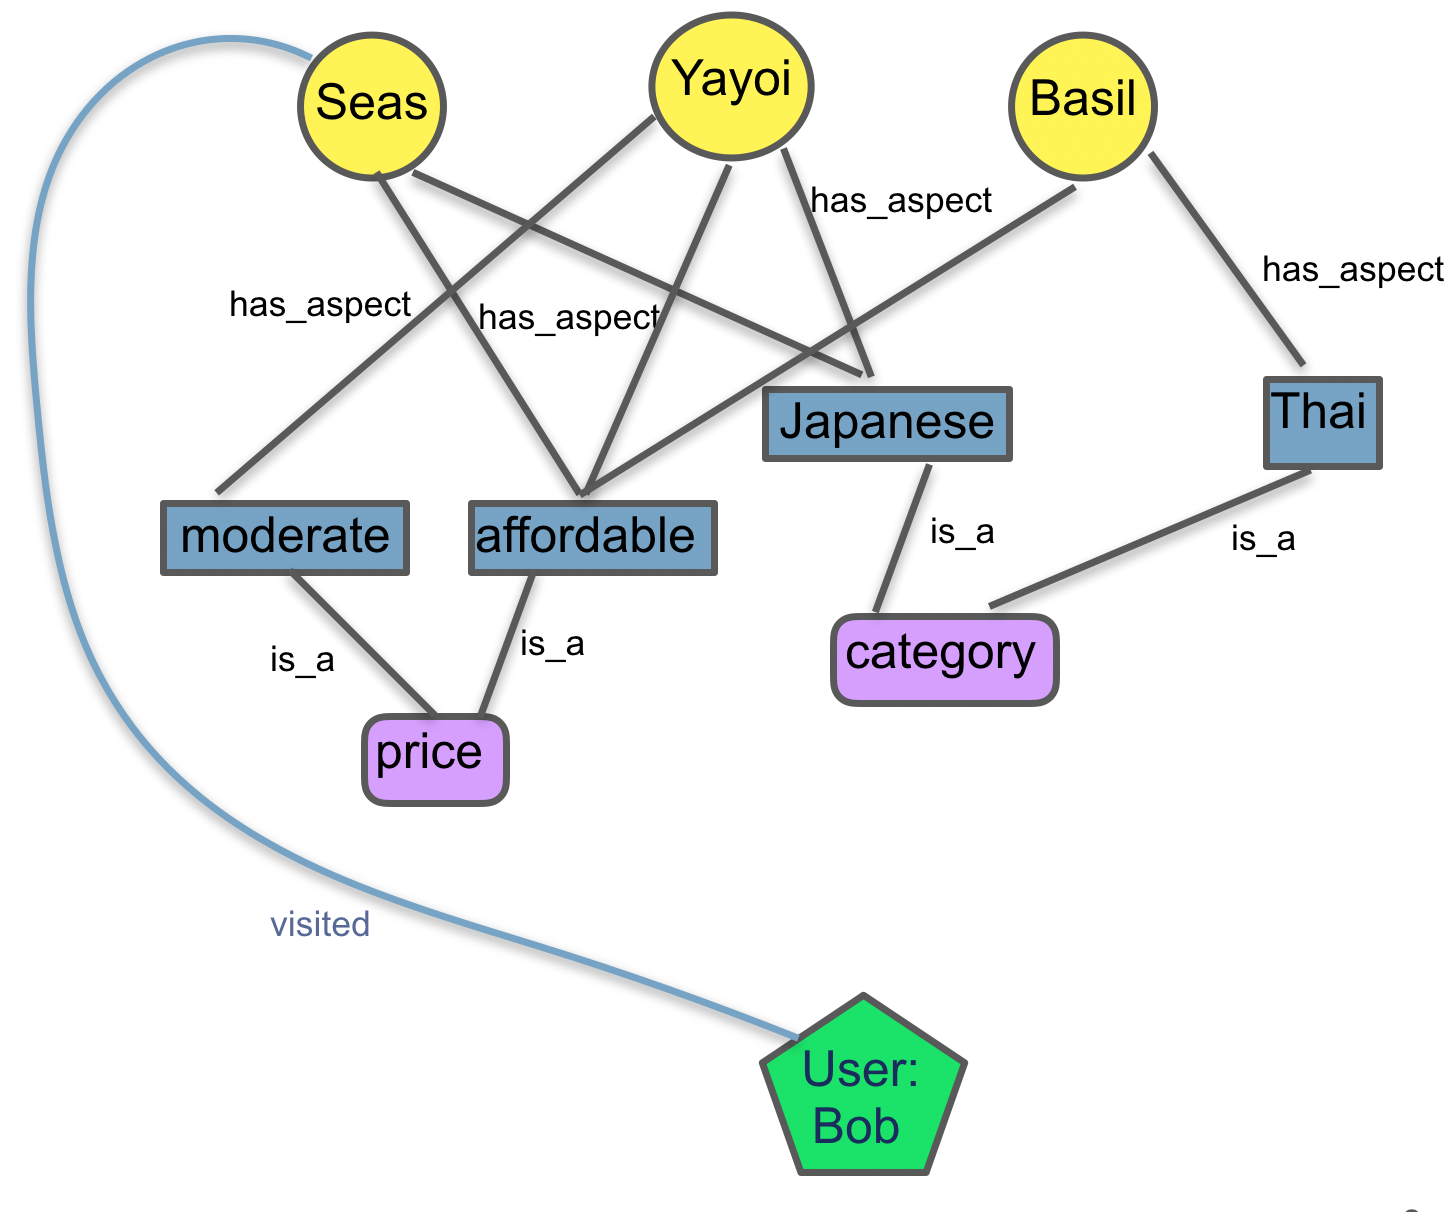
\includegraphics[width=2.2in]{fig/acl19_graph.png}
    \caption{\textbf{Construction of user memory graph}. We omit the memory entity for brevity. In reality, each $r_\text{visited}$ relation has an internal memory entity because a user may have different experiences on the same item at different times.}
\label{chap5:fig:graph}
\vspace{-15pt}
\end{figure}

\begin{figure*}[t]
\centering    
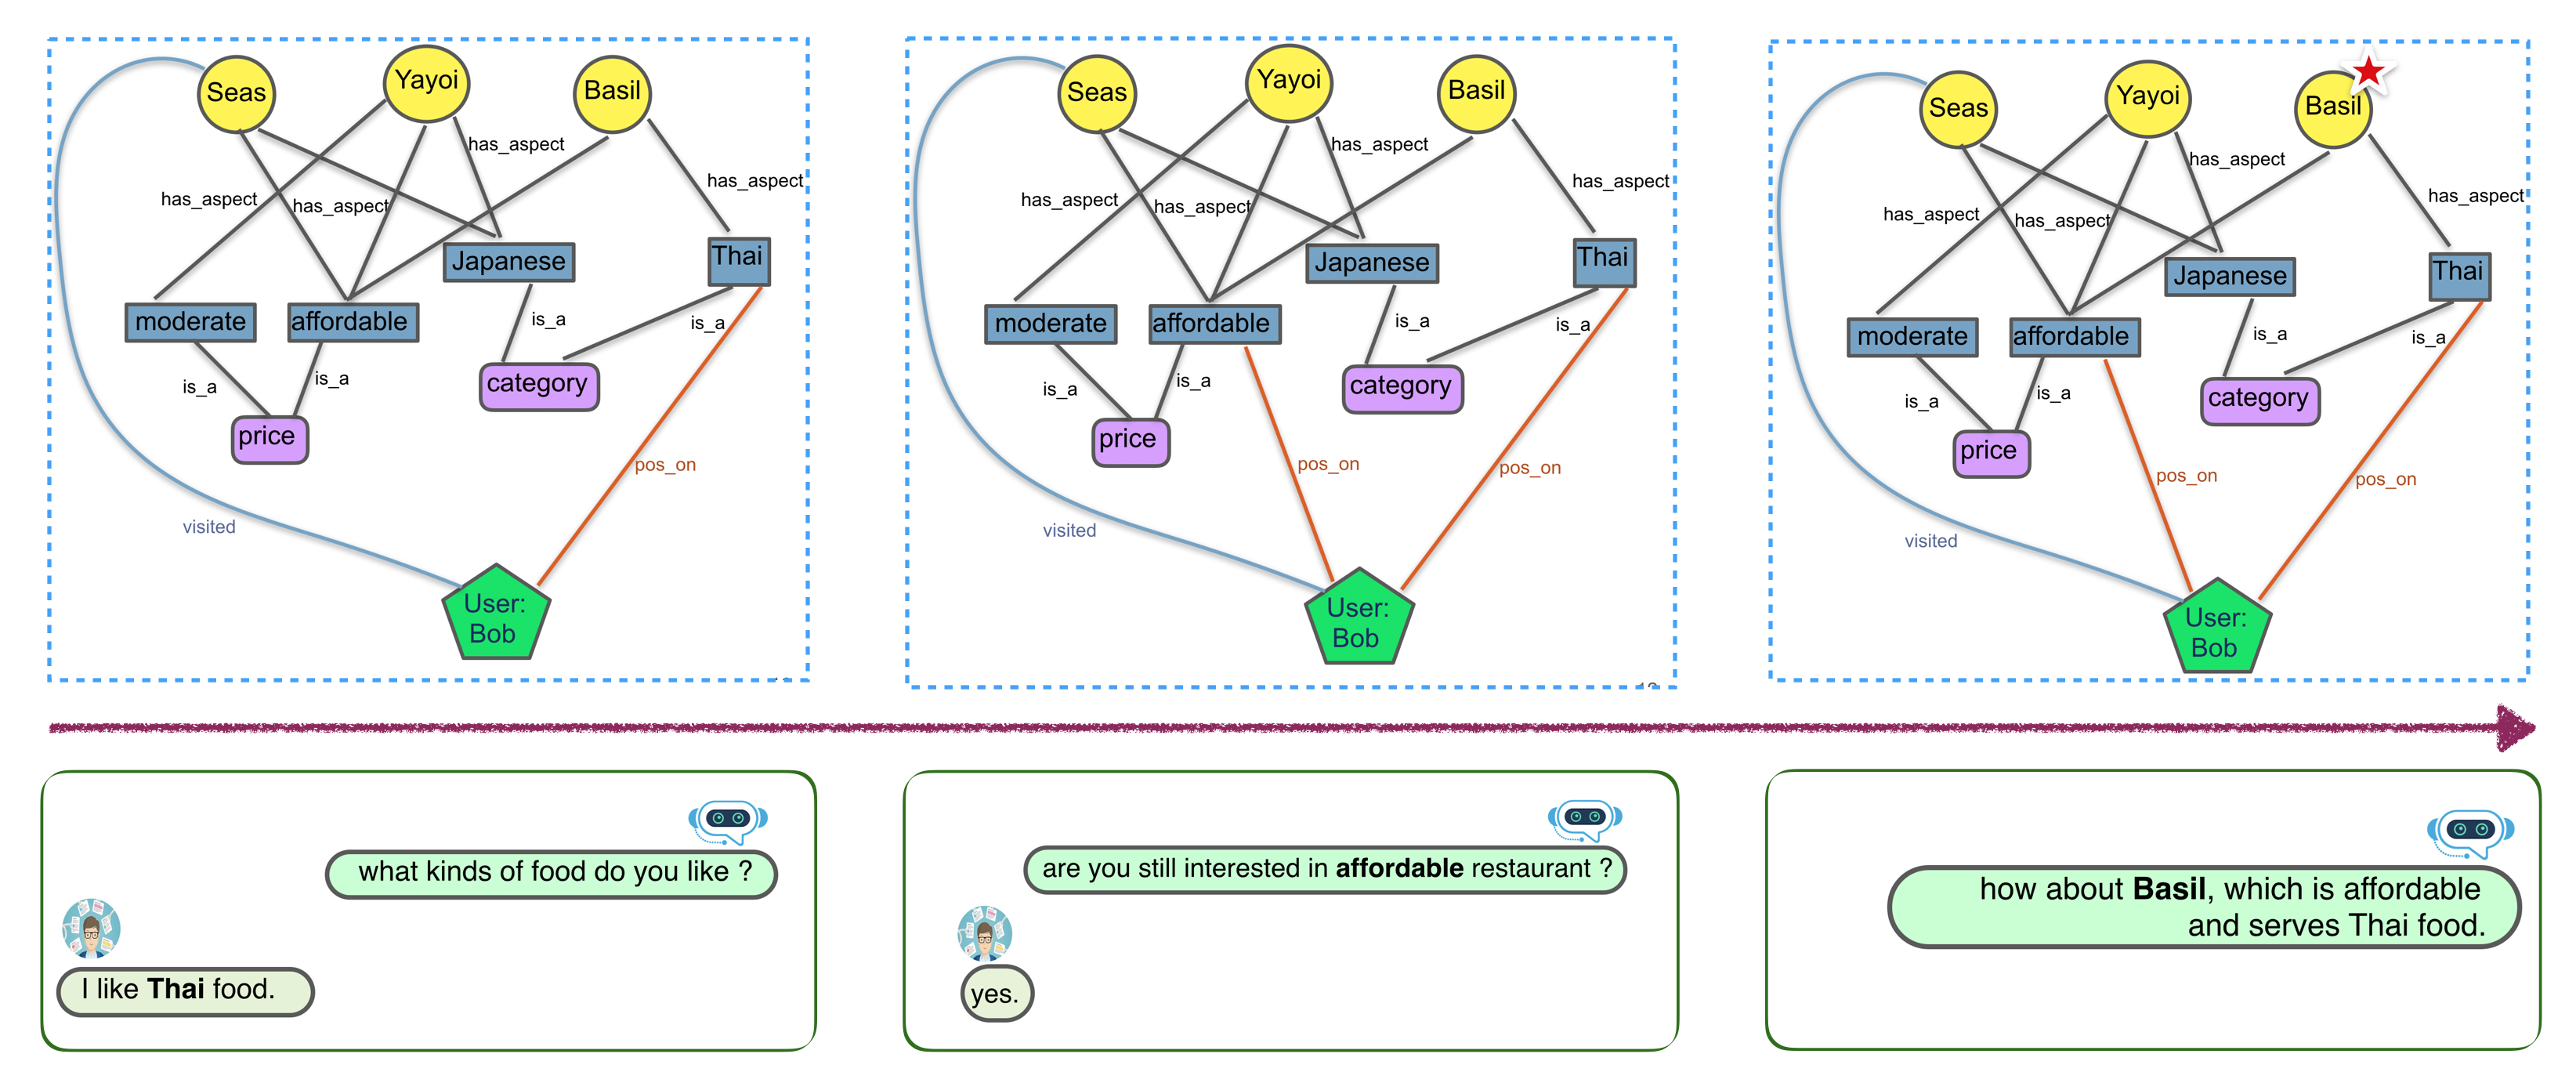
\includegraphics[width=6.0in]{fig/acl19_cum.png}
    \caption{Overview of user memory graph and its accumulation over 3 rounds in a dialogue.}
\label{chap5:fig:cum}
\vspace{-3mm}
\end{figure*}

\section{Graph Reasoner}
\label{chap5:sec:umgr}

We propose a model called User Memory Graph Reasoner (UMGR) to reason the turn-level dialogue policy over the user memory graph.\\ 
\textbf{Input}: the input of UMGR is the past dialogue acts up to the current turn from the user $\boldsymbol{a}$, the updated user memory graph $\mathcal{G}'$, which contains all the knowledge about the items their associated values and slots, and visited items. We further accumulate all updates from the user (e.g., via the assumed results from NLU or state tracking) in the form of last 3 types of relations in Table 4 (Similar to visited items, we add a new memory entity for the current dialogue and then associate all new relations to that memory entity.).\\
\textbf{Output}: UMGR's output is the dialogue policy $\pi=(\hat{y}^\mathcal{A}, \hat{y}^\mathcal{C}, \hat{y}^\mathcal{S}, \hat{y}^\mathcal{V})$ for the current turn, where $\mathcal{A}$, $\mathcal{C}$, $\mathcal{S}$, $\mathcal{V}$ indicate the space of dialogue acts, candidate items, slots and values, respectively.
The predictions from $\hat{y}^\mathcal{C}, \hat{y}^\mathcal{S}$ and $\hat{y}^\mathcal{V}$ essentially provides a ranking over those entity sets.
For example, when $\hat{y}^\mathcal{A}=$ \textit{Recommendation}, the top-1 entity $\argmax_{e_i \in \mathcal{C}}(\hat{y}^\mathcal{C})$ will be provided to the user.
Similarly, $\hat{y}^\mathcal{A}=$ \textit{Open Question} is related to the top-1 slot $\argmax_{e_s \in \mathcal{S}}(\hat{y}^\mathcal{S})$ and $\hat{y}^\mathcal{A}=$ \textit{Yes/no Question} is related to the top-1 value $\argmax_{e_v \in \mathcal{V}}(\hat{y}^\mathcal{V})$.
In this way, all arguments of a dialogue act can be mapped to certain entities in the user memory graph for a structured explanation instead of decoding from latent space.

To enable the reasoning over a user memory graph on-the-fly, we incorporate a Relational Graph Convolutional Networks (R-GCN) \cite{schlichtkrull2018modeling} inside UMGR.
R-GCN is a GCN \cite{kipf2016semi} with typed relations, where each relation is associated with their own weights to enable reasoning over a heterogeneous graph.
UMGR first encodes past dialogue acts $\boldsymbol{a}$ and entities $e \in \mathcal{E}$ into hidden dimensions.
%\vspace{-4mm}
\begin{equation}
\begin{split}
h_a = \text{LSTM}(W^\mathcal{A}(\boldsymbol{a})), \\
h_j^{(0)} = W^\mathcal{E}(e_j),
\end{split}
\end{equation}
where $W^\mathcal{A}$ and $W^\mathcal{E}$ are embedding layers and the past dialogue acts are further encoded by an LSTM encoder.
We further allow on-the-fly reasoning over (new) items by sharing the embedding weights for different items (as a special entity \texttt{<ITEM>}) in $W^\mathcal{E}$. 
Then each entity in the user memory graph is encoded by multiple layers of R-GCN.
\begin{equation}
\begin{split}
h_j^{(l+1)}=\text{LeakyReLU} \Big(\sum_{r \in \mathcal{R}} \sum_{k \in \mathcal{N}_j^r} \frac{1}{\vert \mathcal{N}_j^r \vert} W_r^{(l)} h_j^{(l)}\Big),
\end{split}
\end{equation}
where $h_j^{(l)}$ ($j$ can be any type of entity) is the hidden state of entity $e_j$ in the $l$-th layer of R-GCN. $\mathcal{N}_j^r$ is entity $e_j$'s neighbor in relation type $r$ and $W_r^{(l)}$ is the weights associated with $r$ in the $l$-th layer to transform $h_j^{(l)}$.
The R-GCN layer updates the hidden states of each entity with the incoming messages in the form of their neighbors' hidden states type-by-type.
Then R-GCN sums over all types before passing through the activation.
The hidden states from the last layer of R-GCN is pasted into an aggregation layer.
\begin{equation}
\begin{split}
h^{\text{ag}} = \frac{1}{\vert \mathcal{C} \cup \mathcal{S} \cup \mathcal{V} \vert} \sum_{e_j \in \mathcal{C} \cup \mathcal{S} \cup \mathcal{V}} (W^\text{ag} h_j^{(l+1)} + b^{\text{ag}}),
\end{split}
\end{equation}
where $W^{\text{ag}}$ and $b^{\text{ag}}$ are weights for aggregation layer.
The purpose of having an aggregation layer is to leverage the information in the user memory graph for predicting the dialogue acts, which is a classification problem. The loss for dialogue acts is defined as
\begin{equation}
\begin{split}
\hat{y}^{\mathcal{A}} = \text{Softmax}(W^\mathcal{A} (h_a \oplus h^\text{ag}) +b^\mathcal{A} ), \\
\mathcal{L}^{\mathcal{A}} = \text{CrossEntropyLoss}(\hat{y}^\mathcal{A}, y^\mathcal{A}),
\end{split}
\end{equation}
where $\oplus$ is the concatenation operation and $y^\mathcal{A}$ is the annotated dialogue act.
Further, all item, slot and value entities are trained by log loss for ranking. For example, the loss for candidate items $\mathcal{C}$ is defined as 
\begin{equation}
\begin{split}
\hat{y}_i = \text{Sigmoid}(W^\mathcal{I} h_i +b^{\mathcal{I}} ), \\
\mathcal{L}^\mathcal{C} = \text{LogLoss}(\hat{y}^\mathcal{C}, y^\mathcal{C}).
\end{split}
\end{equation}
Similarly, we obtain loses $\mathcal{L}_\mathcal{S}$, $\mathcal{L}_\mathcal{V}$ for slot entities $\mathcal{S}$ and value entities $\mathcal{V}$, respectively.
Finally, the total loss is the sum over all losses for dialogue acts, items, slots and values: 
\begin{equation}
\begin{split}
\mathcal{L} = \mathcal{L}^\mathcal{A} + \alpha\mathcal{L}^\mathcal{C} + \beta\mathcal{L}^\mathcal{S} + \gamma \mathcal{L}^\mathcal{V},
\end{split}
\end{equation}
where $\alpha, \beta$ and $\gamma$ are hyper-parameters to align losses of different scales.
Note that during training and prediction, all invalid dialogue acts (e.g., user dialogue acts) and entities (e.g., not appear in a user memory graph) are masked out.
As we can see, unlike traditional recommender systems, UMGR does not learn (or ``overfit to'') any prior knowledge about users into the weights. Instead, it reasons the dialogue policy on-the-fly in each turn based on the updated user memory graph.

\chapter{NLP Applications}
\label{chap6:nlp}

In this chapter, I switch to NLP applications that leverage the concept of lifelong representation learning.
I will first focus on tasks in aspect-based sentiment analysis: aspect extraction and aspect sentiment classification.
Then I will discuss its application in question answering.
I will propose some novel review-based QA tasks, with results indicating the importance of lifelong representation.
Next, I will switch to dialogue system.
I will first talk about the conversational version of QA and then switch to a novel type of dialogue system: conversational recommendation, which leverages lifelong graph representation learning for reasoning dialogue policy.
%\section{Product Type Classification}
%\label{chap6:sec:tc}
%\section{Complemenary Entity Recognition}
%\label{chap6:sec:cer}

\section{Sentiment Analysis}
\label{chap6:sec:sa}

Sentiment analysis aims to detect people's the polarity from opinion text \cite{Liu2012}.
More specifically aspect-based sentiment analysis (ABSA) aims to detect the aspects $a$ in opinion texts and their associated polarities $(a, p)$s.
This naturally has two sub-tasks in ABSA: aspect extraction and aspect sentiment classification.

\subsection{-- Aspect Extraction}

One key task of fine-grained sentiment analysis of product reviews is to extract product aspects or features that users have expressed opinions on. This paper focuses on supervised aspect extraction using deep learning. Unlike other highly sophisticated supervised deep learning models, this paper proposes a novel and yet simple CNN model employing two types of pre-trained embeddings for aspect extraction: general-purpose embeddings and domain-specific embeddings. Without using any additional supervision, this model achieves surprisingly good results, outperforming state-of-the-art sophisticated existing methods. To our knowledge, this paper is the first to report such double embeddings based CNN model for aspect extraction and achieve very good results. 

%\section{Introduction}
Aspect extraction is an important task in sentiment analysis \cite{HuL2004} and has many applications \cite{Liu2012}.
It aims to extract opinion targets (or aspects) from opinion text. 
In product reviews, aspects are product attributes or features. 
For example, from ``\textit{Its speed is incredible}'' in a laptop review, it aims to extract ``speed''. 

Aspect extraction has been performed using supervised \cite{Jakob2010,chernyshevich2014ihs,shu2017lifelong} and unsupervised approaches \cite{HuL2004,ZhuangJZ2006,MeiLWSZ2007,QiuLBC2011,yin2016unsupervised,he2017unsupervised}. 
Recently, supervised deep learning models achieved state-of-the-art performances \cite{li2017deep}. Many of these models use handcrafted features, lexicons, and complicated neural network architectures \cite{poria2016aspect,wang2016recursive,wang2017coupled,li2017deep}. 
Although these approaches can achieve better performances than their prior works, there are two other considerations that are also important.
(1) Automated feature (representation) learning is always preferred. 
How to achieve competitive performances without manually crafting features is an important question. 
(2) According to Occam's razor principle \cite{blumer1987occam}, a simple model is always preferred over a complex model.
This is especially important when the model is deployed in a real-life application (e.g., chatbot), where a complex model will slow down the speed of inference. Thus, to achieve competitive performance whereas keeping the model as simple as possible is important. This paper proposes such a model. 

To address the first consideration, we propose a double embeddings mechanism that is shown crucial for aspect extraction.
The embedding layer is the very first layer, where all the information about each word is encoded.
The quality of the embeddings determines how easily later layers (e.g., LSTM, CNN or attention) can decode useful information.
Existing deep learning models for aspect extraction use either a pre-trained general-purpose embedding, e.g., GloVe \cite{pennington2014glove}, or a general review embedding \cite{poria2016aspect}.
However, aspect extraction is a complex task that also requires fine-grained domain embeddings.
For example, in the previous example, detecting ``speed'' may require embeddings of both ``Its'' and ``speed''.
However, the criteria for good embeddings for ``Its'' and ``speed'' can be totally different.
``Its'' is a general word and the general embedding (trained from a large corpus) is likely to have a better representation for ``Its''.
But, ``speed'' has a very fine-grained meaning (e.g., how many instructions per second) in the \textit{laptop} domain, whereas ``speed'' in general embeddings or general review embeddings may mean how many miles per second.
So using in-domain embeddings is important even when the in-domain embedding corpus is not large. 
Thus, we leverage both general embeddings and domain embeddings and let the rest of the network to decide which embeddings have more useful information.

To address the second consideration, we use a pure Convolutional Neural Network (CNN) \cite{lecun1995convolutional} model for sequence labeling.
Although most existing models use LSTM \cite{hochreiter1997long} as the core building block to model sequences \cite{liu2015fine,li2017deep}, we noticed that CNN is also successful in many NLP tasks \cite{kim2014convolutional,zhang2015character,gehring2017convolutional}.
One major drawback of LSTM is that LSTM cells are sequentially dependent.
The forward pass and backpropagation must serially go through the whole sequence, which slows down the training/testing process
\footnote{We notice that a GPU with more cores has no training time gain on a low-dimensional LSTM because extra cores are idle and waiting for the other cores to sequentially compute cells.}.
One challenge of applying CNN on sequence labeling is that convolution and max-pooling operations are usually used for summarizing sequential inputs and the outputs are not well-aligned with the inputs. We discuss the solutions in Section \ref{chap3:sec:model}.

We call the proposed model \underline{D}ual \underline{E}mbeddings \underline{CNN} (DE-CNN).
To the best of our knowledge, this is the first paper that reports a double embedding mechanism and a pure CNN-based sequence labeling model for aspect extraction.

\textbf{Related Work}\\
Sentiment analysis has been studied at document, sentence and aspect levels \cite{Liu2012,Pang2008OMS,Cambria2012}. This work focuses on the aspect level \cite{HuL2004}. Aspect extraction is one of its key tasks, and has been performed using both unsupervised and supervised approaches. 
The unsupervised approach includes methods such as frequent pattern mining \cite{HuL2004,PopescuNE2005}, syntactic rules-based extraction \cite{ZhuangJZ2006,WangBo2008,QiuLBC2011}, topic modeling \cite{MeiLWSZ2007,TitovM2008,Lin2009,Moghaddam2011}, word alignment \cite{KangLiu2013IJCAI} and label propagation \cite{Zhou-wan-xiao:2013:EMNLP,shu2016lifelong}.

Traditionally, the supervised approach \cite{Jakob2010,Mitchell-EtAl:2013:EMNLP,shu2017lifelong} uses Conditional Random Fields (CRF) \cite{Lafferty2001conditional}.
Recently, deep neural networks are applied to learn better features for supervised aspect extraction, e.g., using
LSTM \cite{williams1989learning,hochreiter1997long,liu2015fine} and
attention mechanism \cite{wang2017coupled,he2017unsupervised} together with manual features \cite{poria2016aspect,wang2016recursive}.
Further, \cite{wang2016recursive,wang2017coupled,li2017deep} also proposed aspect and opinion terms co-extraction via a deep network.
They took advantage of the gold-standard opinion terms or sentiment lexicon for aspect extraction.
The proposed approach is close to \cite{liu2015fine}, where only the annotated data for aspect extraction is used. 
However, we will show that our approach is more effective even compared with baselines using additional supervisions and/or resources.

The proposed embedding mechanism is related to cross domain embeddings \cite{bollegala2015unsupervised,bollegala2017think} and domain-specific embeddings \cite{xumeta,Xu2018pro}. 
However, we require the domain of the domain embeddings must exactly match the domain of the aspect extraction task. 
CNN \cite{lecun1995convolutional,kim2014convolutional} is recently adopted for named entity recognition \cite{strubell2017fast}.
CNN classifiers are also used in sentiment analysis \cite{poria2016aspect,chen2017improving}.
We adopt CNN for sequence labeling for aspect extraction because CNN is simple and parallelized.

\textbf{Double Embedding for Sequence Labeling}\\
Following the idea of fusion general and domain-specific embeddings in \ref{chap3}, we have the following CNN-based model for aspect extraction.
%As a counter-example, if the training/testing data is in the \textit{laptop} domain, then embeddings from the \textit{electronics} domain are considered to be out-of-domain embeddings (e.g., the word ``adapter'' may represent different types of adapters in \textit{electronics} rather than exactly a \textit{laptop} adapter). That is, only laptop reviews are considered to be in-domain. 

The proposed model is depicted in Figure \ref{chap3:fig:fr}.
It has 2 embedding layers, 4 CNN layers, a fully-connected layer shared across all positions of words, and a softmax layer over the labeling space $\mathcal{Y}=\{B, I, O\}$ for each position of inputs.
Note that an aspect can be a phrase and $B$, $I$ indicate the beginning word and non-beginning word of an aspect phrase and $O$ indicates non-aspect words.

\begin{figure}[t]
\centering    
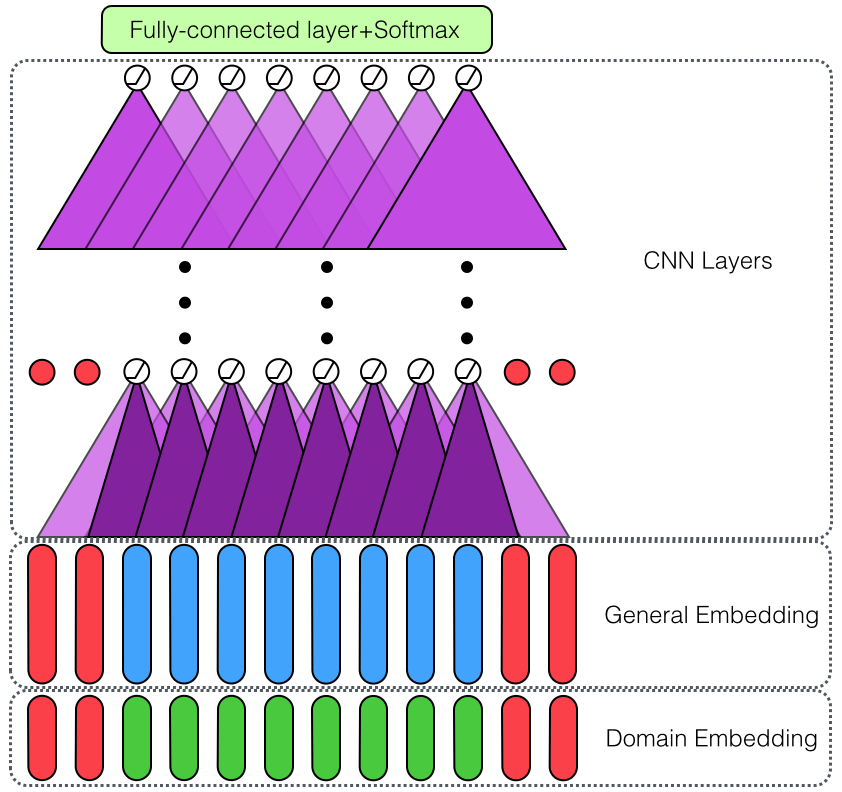
\includegraphics[width=3in]{fig/acl18_fig.png}
    \caption{Overview of DE-CNN: red vectors are zero vectors; purple triangles are CNN filters. }
    \label{chap3:fig:fr}
\end{figure}

A CNN layer has many 1D-convolution filters and each (the $r$-th) filter has a fixed kernel size $k=2c+1$ and performs the following convolution operation and ReLU activation: 
%\vspace{-0.5cm}
\begin{equation}
x_{i,r}^{(l+1)}=\max\bigg(0, (\sum_{j=-c}^c w_{j,r}^{(l)} x_{i+j}^{(l)})+b_r^{(l)}\bigg),
\end{equation}
%\vspace{-0.3cm}
%\noindent
where $l$ indicates the $l$-th CNN layer. 
We apply each filter to all positions $i=1:n$.
So each filter computes the representation for the $i$-th word along with $2c$ nearby words in its context.  
Note that we force the kernel size $k$ to be an odd number and set the stride step to be 1 and further pad the left $c$ and right $c$ positions with all zeros.  
In this way, the output of each layer is well-aligned with the original input $\mathbf{x}$ for sequence labeling purposes.
For the first ($l=1$) CNN layer, we employ two different filter sizes. 
For the rest 3 CNN ($l \in \{2, 3, 4\}$) layers, we only use one filter size.
We will discuss the details of the hyper-parameters in the experiment section.
Finally, we apply a fully-connected layer with weights shared across all positions and a softmax layer to compute label distribution for each word.
The output size of the fully-connected layer is $|\mathcal{Y}|=3$.
We apply dropout after the embedding layer and each ReLU activation.
Note that we do not apply any max-pooling layer after convolution layers because a sequence labeling model needs good representations for every position and max-pooling operation mixes the representations of different positions, which is undesirable (we show a max-pooling baseline in the next section).


\textbf{Aspect Extraction from Pre-trained Language Model}\\
Further, based on technique of post-training in \ref{chap4}, we can also use the weights of pre-train or post-training for aspect extraction with an extra layer of token type classification.

We only extend BERT with one extra task-specific layer and fine-tune BERT on each end task.
This can be illustrated in the second sub-figure in \ref{chap6:fig:overview}.

\begin{figure}[t]
\centering
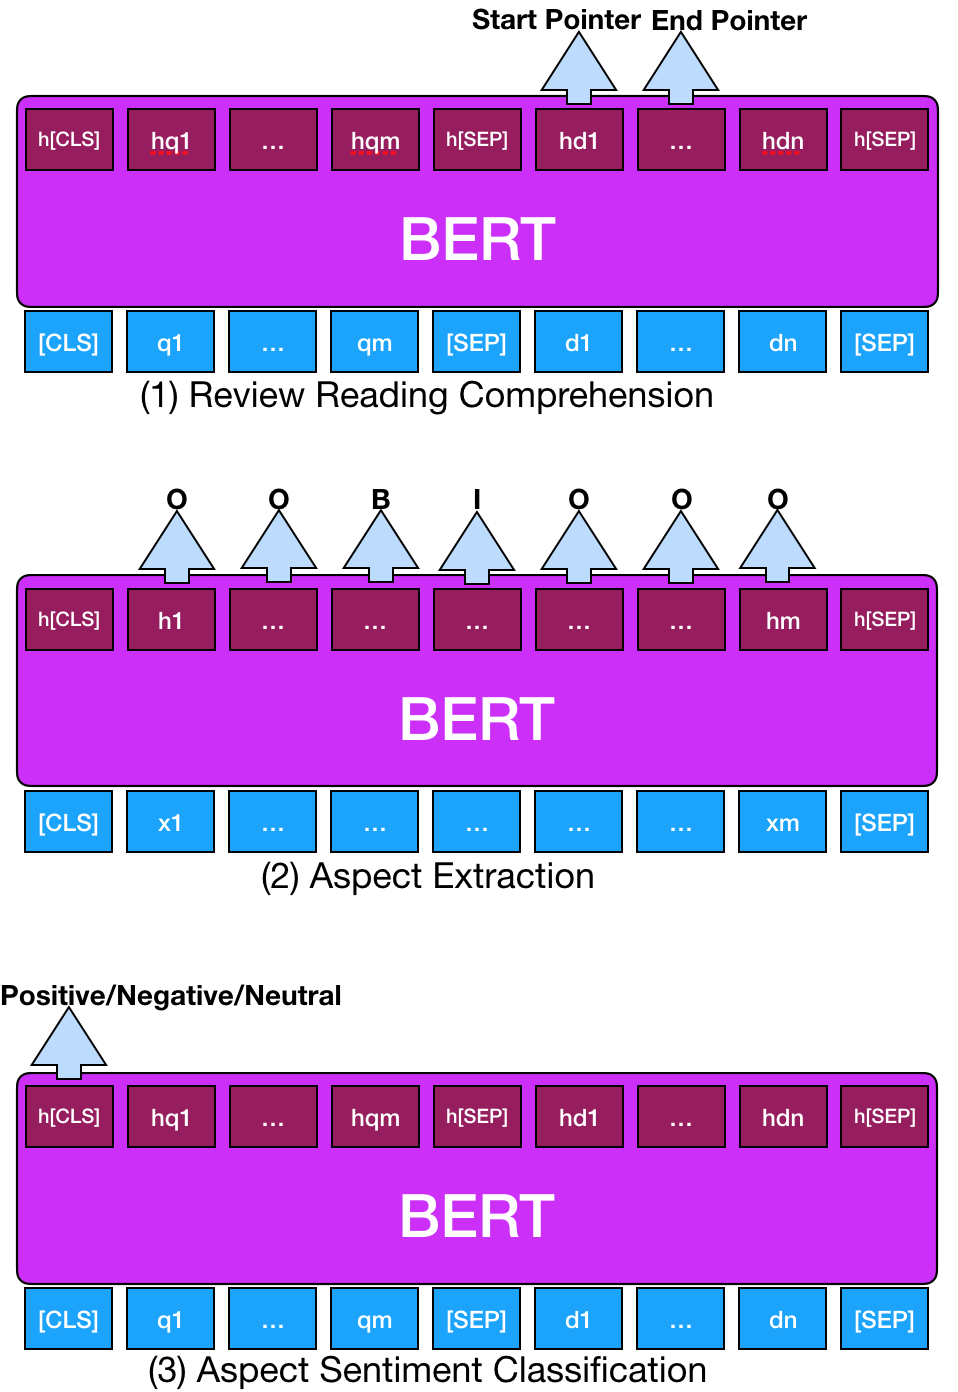
\includegraphics[width=3.0in]{fig/naacl19_overview.png}
    \caption{Overview of BERT settings for review reading comprehension (RRC), aspect extraction (AE) and aspect sentiment classification (ASC).}
\label{chap6:fig:overview}
\vspace{-3mm}
\end{figure}
%As a core task in ABSA, aspect extraction (AE) aims to find aspects that reviewers have expressed opinions on \cite{hu2004mining}. 
%In supervised settings, it is typically modeled as a sequence labeling task, where each token from a sentence is labeled as one of $\{\textit{\underline{B}egin}, \textit{\underline{I}nside}, \textit{\underline{O}utside}\}$. A continuous chunk of tokens that are labeled as one \textit{B} and followed by zero or more \textit{I}s forms an aspect.
The input sentence with $m$ words is constructed as $x=(\texttt{[CLS]}, x_1, \dots, x_m, \texttt{[SEP]})$.
After $h=\text{BERT}(x)$, we apply a dense layer and a softmax for each position of the sequence: $l_3=\text{softmax}(W_3 \cdot h + b_3)$, where $W_3 \in \mathbb{R}^{3*r_h}$ and $b_3 \in \mathbb{R}^3$ (3 is the total number of labels (\textit{BIO})).  Softmax is applied along the dimension of labels for each position and $l_3 \in [0, 1]^{3*|x|}$. The labels are predicted as taking argmax function at each position of $l_3$ and the loss function is the averaged cross entropy across all positions of a sequence.

AE is a task that requires intensive domain knowledge (e.g., knowing that ``screen'' is a part of a laptop). Previous study \cite{xu_acl2018} has shown that incorporating domain word embeddings greatly improve the performance. 
Adapting BERT's general language models to domain reviews is crucial for AE,
as shown in Sec. %\ref{chap6:sec:exp}.


\textbf{Datasets}\\

\begin{table}[t]
    \label{tab:dataset} 
    \centering
    \scalebox{0.8}{
        \begin{tabular}{c|c|c}
        \hline
            {\bf Description}  &{\bf Training }        &{\bf Testing }  \\
                               &{\bf \#S./\#A.} &{\bf \#S./\#A.}  \\\hline
            SemEval-14 Laptop  &3045/2358              &800/654\\\hline
            SemEval-16 Restaurant&2000/1743            &676/622\\\hline
        \end{tabular}
    }
    \caption{Dataset description with the number of sentences(\#S.) and number of aspect terms(\#A.)}
\end{table}

\textbf{Results}\\
Following the experiments of a recent aspect extraction paper \cite{li2017deep},
we conduct experiments on two benchmark datasets from SemEval challenges \cite{pontiki2014SemEval,pontiki2016semeval} as shown in Table \ref{tab:dataset}. 
The first dataset is from the \textit{laptop} domain on subtask 1 of SemEval-2014 Task 4.
The second dataset is from the \textit{restaurant} domain on subtask 1 (slot 2) of SemEval-2016 Task 5.
These two datasets consist of review sentences with aspect terms labeled as spans of characters.
We use NLTK\footnote{\url{http://www.nltk.org/} } to tokenize each sentence into a sequence of words. 

For the general-purpose embeddings, we use the glove.840B.300d embeddings \cite{pennington2014glove}, which are pre-trained from a corpus of 840 billion tokens that cover almost all web pages. These embeddings have 300 dimensions.
For domain-specific embeddings, we collect a laptop review corpus and a restaurant review corpus and use fastText \cite{bojanowski2016enriching} to train domain embeddings.  
The laptop review corpus contains all laptop reviews from the Amazon Review Dataset \cite{he2016ups}.
The restaurant review corpus is from the Yelp Review Dataset Challenge \footnote{\url{https://www.yelp.com/dataset/challenge} }.
We only use reviews from restaurant categories that the second dataset is selected from \footnote{\url{http://www.cs.cmu.edu/~mehrbod/RR/Cuisines.wht} }.
We set the embedding dimensions to 100 and the number of iterations to 30 (for a small embedding corpus, embeddings tend to be under-fitted), and keep the rest hyper-parameters as the defaults in fastText.
We further use fastText to compose out-of-vocabulary word embeddings via subword N-gram embeddings.

\textbf{Baseline Methods for DE-CNN}\\
We perform a comparison of DE-CNN with three groups of baselines using the standard evaluation of the datasets\footnote{\url{http://alt.qcri.org/semeval2014/task4}} \footnote{\url{http://alt.qcri.org/semeval2016/task5}}.
The results of the first two groups are copied from \cite{li2017deep}.
The first group uses single-task approaches.

\textbf{CRF} is conditional random fields with basic features\footnote{\url{http://sklearn-crfsuite.readthedocs.io/en/latest/tutorial.html} } and GloVe word embedding\cite{pennington2014glove}.

\textbf{IHS\_RD} \cite{chernyshevich2014ihs} and \textbf{NLANGP} \cite{toh2016nlangp} are best systems in the original challenges \cite{pontiki2014SemEval,pontiki2016semeval}.

\textbf{WDEmb} \cite{yin2016unsupervised} enhanced CRF with word embeddings, linear context embeddings and dependency path embeddings as input.

\textbf{LSTM} \cite{liu2015fine,li2017deep} is a vanilla BiLSTM.

\textbf{BiLSTM-CNN-CRF} \cite{Reimers:2017:EMNLP} is the state-of-the-art from the Named Entity Recogntion (NER) community. We use this baseline\footnote{\url{https://github.com/UKPLab/emnlp2017-bilstm-cnn-crf} } to demonstrate that a NER model may need further adaptation for aspect extraction.

The second group uses multi-task learning and also take advantage of gold-standard opinion terms/sentiment lexicon.

\textbf{RNCRF} \cite{wang2016recursive} is a joint model with a dependency tree based recursive neural network and CRF for aspect and opinion terms co-extraction. 
Besides opinion annotations, it also uses handcrafted features.

\textbf{CMLA} \cite{wang2017coupled} is a multi-layer coupled-attention network that also performs aspect and opinion terms co-extraction. It uses gold-standard opinion labels in the training data.

\textbf{MIN} \cite{li2017deep} is a multi-task learning framework that has (1) two LSTMs for jointly extraction of aspects and opinions, and (2) a third LSTM for discriminating sentimental and non-sentimental sentences. 
A sentiment lexicon and high precision dependency rules are employed to find opinion terms. 

The third group is the variations of DE-CNN.

\textbf{GloVe-CNN} only uses glove.840B.300d to show that domain embeddings are important. 

\textbf{Domain-CNN} does not use the general embeddings to show that domain embeddings alone are not good enough as the domain corpus is limited for training good general words embeddings.

\textbf{MaxPool-DE-CNN} adds max-pooling in the last CNN layer. We use this baseline to show that the max-pooling operation used in the traditional CNN architecture is harmful to sequence labeling.

\textbf{DE-OOD-CNN} replaces the domain embeddings with out-of-domain embeddings to show that a large out-of-domain corpus is not a good replacement for a small in-domain corpus for domain embeddings.
We use all \textit{electronics} reviews as the out-of-domain corpus for the \textit{laptop} and all the Yelp reviews for \textit{restaurant}.

\textbf{DE-Google-CNN} replaces the glove embeddings with GoogleNews embeddings\footnote{\url{https://code.google.com/archive/p/word2vec/} }, which are pre-trained from a smaller corpus (100 billion tokens). We use this baseline to demonstrate that general embeddings that are pre-trained from a larger corpus performs better.

\textbf{DE-CNN-CRF} replaces the softmax activation with a CRF layer\footnote{\url{https://github.com/allenai/allennlp}}. We use this baseline to demonstrate that CRF may not further improve the challenging performance of aspect extraction.

\textbf{Hyper-parameters of DE-CNN}\\
We hold out 150 training examples as validation data to decide the hyper-parameters.
The first CNN layer has 128 filters with kernel sizes $k=3$ (where $c=1$ is the number of words on the left (or right) context) and 128 filters with kernel sizes $k=5$ ($c=2$).
The rest 3 CNN layers have 256 filters with kernel sizes $k=5$ ($c=2$) per layer.
The dropout rate is 0.55 and the learning rate of Adam optimizer \cite{kingma2014adam} is 0.0001 because CNN training tends to be unstable.

\begin{table}[t]
    \label{chap6:tab:result} 
    \centering
    \scalebox{0.85}{
        \begin{tabular}{c||c|c}
        \hline
        {\bf Model} &{\bf Laptop }  &{\bf Restaurant }  \\\hline
        CRF         &74.01      &69.56  \\
        IHS\_RD     &74.55      &-      \\
        NLANGP      &-          &72.34  \\
        WDEmb       &75.16      &-      \\
        LSTM        &75.25      &71.26  \\
		BiLSTM-CNN-CRF &77.8 & 72.5\\
        \hline
        RNCRF       &78.42 &-      \\
        CMLA        &77.80      &-      \\
        MIN         &77.58      &73.44  \\
        \hline
        \hline
        GloVe-CNN & 77.67 & 72.08\\
        Domain-CNN & 78.12 & 71.75\\
        MaxPool-DE-CNN & 77.45 & 71.12\\
        DE-LSTM & 78.73 & 72.94 \\
        DE-OOD-CNN & 80.21 & 74.2 \\
		DE-Google-CNN & 78.8 & 72.1 \\
		DE-CNN-CRF & 80.8 & 74.1 \\
        DE-CNN &\textbf{81.59}* &\textbf{74.37}* \\
        \hline
        \end{tabular}
    }
    \caption{Comparison results in F$_1$ score: numbers in the third group are averaged scores of 5 runs as in \cite{li2017deep}. * indicates the result is statistical significant at the level of 0.05.}
\end{table}

\textbf{Results and Analysis}\\
Table \ref{chap6:tab:result} shows that DE-CNN performs the best. 
The double embedding mechanism improves the performance and in-domain embeddings are important. 
We can see that using general embeddings (GloVe-CNN) or domain embeddings (Domain-CNN) alone gives inferior performance. 
We further notice that the performance on \textit{Laptops} and \textit{Restaurant} domains are quite different. 
\textit{Laptops} has many domain-specific aspects, such as ``adapter''. 
So the domain embeddings for \textit{Laptops} are better than the general embeddings. 
The \textit{Restaurant} domain has many very general aspects like ``staff'', ``service'' that do not deviate much from their general meanings. 
So general embeddings are not bad. 
Max pooling is a bad operation as indicated by MaxPool-DE-CNN since the max pooling operation loses word positions.
DE-OOD-CNN's performance is poor, indicating that making the training corpus of domain embeddings to be exactly in-domain is important.
DE-Google-CNN uses a much smaller training corpus for general embeddings, leading to poorer performance than that of DE-CNN.
Surprisingly, we notice that the CRF layer (DE-CNN-CRF) does not help.
In fact, the CRF layer can improve 1-2\% when the laptop's performance is about 75\%.
But it doesn't contribute much when laptop's performance is above 80\%. 
CRF is good at modeling label dependences (e.g., label $I$ must be after $B$), but many aspects are just single words and the major types of errors (mentioned later) do not fall in what CRF can solve.
Note that we did not tune the hyperparameters of DE-CNN-CRF for practical purpose because training the CRF layer is extremely slow. 

One important baseline is BiLSTM-CNN-CRF, which is markedly worse than our method. 
We believe the reason is that this baseline leverages dependency-based embeddings\cite{levy2014dependency}, 
which could be very important for NER.
NER models may require further adaptations (e.g., domain embeddings) for opinion texts. 

DE-CNN has two major types of errors.
One type comes from inconsistent labeling (e.g., for the restaurant data, the same aspect is sometimes labeled and sometimes not). 
Another major type of errors comes from unseen aspects in test data that require the semantics of the conjunction word ``and'' to extract. For example, if A is an aspect and when ``A and B'' appears, B should also be extracted but not.
We leave this to future work.


We further conduct experiments for the results of DE-CNN with language model (BERT) based methods.

\textbf{Hyper-parameters of BERT}\\
\label{chap6:sec:hyp}
We adopt $\textbf{BERT}_\textbf{BASE}$ (uncased) as the basis for all experiments\footnote{We expect $\textbf{BERT}_\textbf{LARGE}$ to have better performance but leave that to future work due to limited computational power.}.~Since post-training may take a large footprint on GPU memory (as BERT pre-training), we leverage FP16 computation\footnote{\url{https://docs.nvidia.com/deeplearning/sdk/mixed-precision-training/index.html}} to reduce the size of both the model and hidden representations of data.~We set a static loss scale of 2 in FP16, which can avoid any over/under-flow of floating point computation.
The maximum length of post-training is set to 320 with a batch size of 16 for each type of knowledge.~The number of sub-batch $u$ is set to 2, which is good enough to store each sub-batch iteration into a GPU memory of 11G. We use Adam optimizer and set the learning rate to be 3e-5.
We train 70,000 steps for the laptop domain and 140,000 steps for the restaurant domain, which roughly have one pass over the pre-processed data on the respective domain.

\textbf{Baseline Methods for BERT}\\
\textbf{BERT} leverages the vanilla BERT pre-trained weights and fine-tunes on all 3 end tasks. We use this baseline to answer RQ2 and show that BERT's pre-trained weights alone have limited performance gains on review-based tasks.\\
\textbf{BERT-DK} post-trains BERT's weights only on domain knowledge (reviews) and fine-tunes on the 3 end tasks. We use BERT-DK and the following BERT-MRC to answer RQ3.\\
\textbf{BERT-MRC} post-trains BERT's weights on SQuAD 1.1 and then fine-tunes on the 3 end tasks.\\
\textbf{BERT-PT} (proposed method) post-trains BERT's weights using the joint post-training algorithm in Section \ref{chap4:sec:post-training} and then fine-tunes on the 3 end tasks.

\textbf{Discussion of Results}

\begin{table}
    \centering
    \scalebox{0.9}{
        \begin{tabular}{l||c|c}
        \hline
        {\bf Domain} & {\bf Laptop} & {\bf Rest.} \\
        \hline
        {\bf Methods} & {\bf F1 } & {\bf F1 } \\
        \hline
        \begin{tabular}{@{}l@{}}DE-CNN\cite{xu_acl2018}\end{tabular} & 81.59 & 74.37 \\
        \hline
        BERT  & 79.28 & 74.1 \\
        BERT-DK & 83.55 & 77.02 \\
        BERT-MRC & 81.06 & 74.21 \\
        BERT-PT & \textbf{84.26} & \textbf{77.97} \\
        \hline
        \end{tabular}
    }
	\caption{AE in F1.}
\label{chap6:tbl:result_ae}
\vspace{-5mm}
\end{table}

we found that great performance boost comes mostly from domain knowledge post-training, which indicates that contextualized representations of domain knowledge are very important for AE. BERT-MRC has almost no improvement on restaurant, which indicates Wikipedia may have no knowledge about aspects of restaurant.
We suspect that the improvements on laptop come from the fact that many answer spans in SQuAD are noun terms, which bear a closer relationship with laptop aspects.
Errors mostly come from annotation inconsistency and boundaries of aspects (e.g., apple OS is predicted as OS). Restaurant suffers from rare aspects like the names of dishes.

%\textbf{Conclusion}\\
%We propose a CNN-based aspect extraction model with a double embeddings mechanism without extra supervision.
%Experimental results demonstrated that the proposed method outperforms state-of-the-art methods with a large margin.

\subsection{-- Aspect Sentiment Classification}

As a subsequent task of AE, aspect sentiment classification (ASC) aims to classify the sentiment polarity (positive, negative, or neutral) expressed on an aspect extracted from a review sentence.
There are two inputs to ASC: an aspect and a review sentence mentioning that aspect.

Let $x=(\texttt{[CLS]}, q_1, \dots, q_m, \texttt{[SEP]}, d_1, \dots, \\ d_n, \texttt{[SEP]})$, where $q_1, \dots, q_m$ now is an aspect (with $m$ tokens) and $d_1, \dots, d_n$ is a review sentence containing that aspect.
After $h=\text{BERT}(x)$, we leverage the representations of \texttt{[CLS]} $h_{\text{[CLS]}}$, which is the aspect-aware representation of the whole input.
The distribution of polarity is predicted as $l_4=\text{softmax}(W_4 \cdot h_{\text{[CLS]}} + b_4)$, where $W_4 \in \mathbb{R}^{3*r_h}$ and $b_4 \in \mathbb{R}^3$ (3 is the number of polarities). Softmax is applied along the dimension of labels on \texttt{[CLS]}: $l_4 \in [0, 1]^{3}$.
Training loss is the cross entropy on the polarities.

As a summary of these tasks, insufficient supervised training data significantly limits the performance gain across these 3 review-based tasks.~Although BERT's pre-trained weights strongly boost the performance of many other NLP tasks on formal texts, we observe in Sec. \ref{chap6:sec:exp} that BERT's weights only result in limited gain or worse performance compared with existing baselines.
In the next section, we introduce the post-training step to boost the performance of all these 3 tasks.

\textbf{datasets}\\
For ASC, we use SemEval 2014 Task 4 for both laptop and restaurant as existing research frequently uses this version. We use 150 examples from the training set of all these datasets for validation.

\begin{table}[t]
    \centering
    \scalebox{0.78}{
        \begin{tabular}{l||c c|c c}
        \hline
        {\bf Domain} & {\bf Laptop} & & {\bf Rest.} & \\
        \hline
        {\bf Methods} & \bf{Acc.} & \bf{MF1} & \bf{Acc.} & \bf{MF1} \\
        \hline
        \begin{tabular}{@{}l@{}}
        MGAN \cite{li2018exploiting}\end{tabular} & 76.21 & 71.42 & 81.49 & 71.48 \\
        \hline
        BERT & 75.29 & 71.91 & 81.54 & 71.94 \\
        BERT-DK & 77.01 & 73.72 & 83.96 & 75.45 \\
        BERT-MRC & 77.19 & 74.1 & 83.17 & 74.97 \\
        BERT-PT & 78.07 & \textbf{75.08} & 84.95 & \textbf{76.96} \\
        \hline
        \end{tabular}
    }
	\caption{ASC in Accuracy and Macro-F1(MF1).}
\label{chap6:tbl:result_asc}
\vspace{-5mm}
\end{table}

\textbf{Compared Methods and Evaluation Metrics}\\
\textbf{MGAN} \cite{li2018exploiting} reaches the state-of-the-art ASC on SemEval 2014 task 4.
We compute both accuracy and Macro-F1 over 3 classes of polarities, where Macro-F1 is the major metric as the imbalanced classes introduce biases on accuracy.~To be consistent with existing research \cite{tang2016aspect}, examples belonging to the \textit{conflict} polarity are dropped due to a very small number of examples.


\textbf{Results Discussion}\\
ASC, we observed that large-scale annotated MRC data is very useful.
We suspect the reason is that ASC can be interpreted as a special MRC problem, where all questions are about the polarity of a given aspect.
MRC training data may help BERT to understand the input format of ASC given their closer input formulation.
Again, domain knowledge post-training also helps ASC.
ASC tends to have more errors as the decision boundary between the negative and neutral examples is unclear (e.g., even annotators may not sure whether the reviewer shows no opinion or slight negative opinion when mentioning an aspect).
Also, BERT-PT has the problem of dealing with one sentence with two opposite opinions (``The screen is good but not for windows.''). We believe that such training examples are rare.


\section{Question Answering}
\label{chap6:sec:qa}

In this section, we discuss the usage of post-training to question answering.
We focus on a novel review-based task called review reading comprehension (RRC).

\subsection{-- Motivation}
Question-answering plays an important role in e-commerce as it allows potential customers to actively seek crucial information about products or services to help their purchase decision making. 
Inspired by the recent success of machine reading comprehension (MRC) on formal documents, this paper explores the potential of turning customer reviews into a large source of knowledge that can be exploited to answer user questions.~We call this problem \textit{\underline{R}eview \underline{R}eading \underline{C}omprehension} (RRC).~To the best of our knowledge, no existing work has been done on RRC. In this work, we first build an RRC dataset called ReviewRC based on a popular benchmark for aspect-based sentiment analysis.~Since ReviewRC has limited training examples for RRC (and also for aspect-based sentiment analysis), we then explore a novel post-training approach on the popular language model BERT to enhance the performance of fine-tuning of BERT for RRC.
To show the generality of the approach, the proposed post-training is also applied to some other review-based tasks such as aspect extraction and aspect sentiment classification in aspect-based sentiment analysis. 

For online commerce, question-answering (QA) serves either as a standalone application of customer service or as a crucial component of a dialogue system that answers user questions.
Many intelligent personal assistants (such as Amazon Alexa and Google Assistant) support online shopping by allowing the user to speak directly to the assistants. 
One major hindrance for this mode of shopping is that such systems have limited capability to answer user questions about products (or services), which are vital for customer decision making.
As such, an intelligent agent that can automatically answer customers' questions is very important for the success of online businesses.

Given the ever-changing environment of products and services, it is very hard, if not impossible, to pre-compile an up-to-date and reliable knowledge base to cover a wide assortment of questions that customers may ask, such as in factoid-based KB-QA \cite{xu2016question,fader2014open,kwok2001scaling,yin2015neural}.
As a compromise, many online businesses leverage community question-answering (CQA) \cite{mcauley2016addressing} to crowdsource answers from existing customers. However, the problem with this approach is that many questions are not answered, and if they are answered, the answers are delayed, which is not suitable for interactive QA.
In this paper, we explore the potential of using product reviews as a large source of user experiences that can be exploited to obtain answers to user questions. Although there are existing studies that have used information retrieval (IR) techniques \cite{mcauley2016addressing,yu2018aware} to find a whole review as the response to a user question, giving the whole review to the user is undesirable as it is quite time-consuming for the user to read it.

Inspired by the success of \underline{M}achine \underline{R}eading \underline{C}omphrenesions (MRC) \cite{rajpurkar2016squad,rajpurkar2018know}, we propose a novel task called \underline{R}eview \underline{R}eading \underline{C}omprehension (RRC) as following.

\textbf{Problem Definition}: Given a question $q=(q_1, \dots, q_m)$ from a customer (or user) about a product and a review $d=(d_1, \dots, d_n)$ for that product containing the information to answer $q$, find a sequence of tokens (a text span) $a=(d_s, \dots, d_e)$ in $d$ that answers $q$ correctly, where $1 \le s \le n$, $1\le e \le n$, and $s\le e$.

\label{sec:intro}
\begin{table}
    \centering
    \scalebox{0.87}{
        \begin{tabular}{|l|}
            \hline
            {\bf Questions}\\
            \hline
            Q1: Does it have an internal hard drive ?\\
            Q2: How large is the internal hard drive ?\\
            Q3: is the capacity of the internal hard drive OK ?\\
            \hline
            {\bf Review}\\
            Excellent value and a must buy for someone \\
            looking for a Macbook . You ca n't get any \\
            better than this price and it \textbf{come with}\textsubscript{A1} an\\
            internal disk drive . All the newer MacBooks\\
            do not . Plus you get \textbf{500GB}\textsubscript{A2} which is also a\\
            \textbf{great}\textsubscript{A3} feature . Also , the resale value on \\
            this will keep . I highly recommend you get one \\
            before they are gone .\\
            \hline
        \end{tabular}
    }
	\caption{An example of review reading comprehension: we show 3 questions and their corresponding answer spans from a review.}
    \label{chap6:tbl:example}
\end{table}

A sample \emph{laptop} review is shown in Table \ref{chap6:tbl:example}. 
We can see that customers may not only ask factoid questions such as the specs about some aspects of the laptop as in the first and second questions but also subjective or opinion questions about some aspects (capacity of the hard drive), as in the third question.
RRC poses some \textit{domain challenges} compared to the traditional MRC on Wikipedia, such as the need for rich product knowledge, informal text, and fine-grained opinions (there is almost no subjective content in Wikipedia articles). Research also shows that yes/no questions are very frequent for products with complicated specifications \cite{mcauley2016addressing,Xu2018pro}.

To the best of our knowledge, no existing work has been done in RRC. This work first builds an RRC dataset called ReviewRC, using reviews from SemEval 2016 Task 5\footnote{\url{http://alt.qcri.org/semeval2016/task5/}. We choose these review datasets to align RRC with existing research on sentiment analysis.}, which is a popular dataset for aspect-based sentiment analysis (ABSA) \cite{hu2004mining} in the domains of \emph{laptop} and \emph{restaurant}.
We detail ReviewRC in Sec. \ref{chap6:sec:exp}.
Given the wide spectrum of domains (types of products or services) in online businesses and the prohibitive cost of annotation, ReviewRC can only be considered to have a limited number of annotated examples for supervised training, which still leaves the domain challenges partially unresolved.

To simplify the writing, we refer MRC as a general-purpose RC task on formal text (non-review) and RRC as an end-task specifically focused on reviews.), where the former enhances domain-awareness and the latter strengthens MRC task-awareness.
Although BERT gains great success on SQuAD, this success is based on the huge amount of training examples of SQuAD (100,000+).
This amount is large enough to ameliorate the flaws of BERT that has almost no questions on the left side and no textual span predictions based on both the question and the document on the right side.
However, a small amount of fine-tuning examples is not sufficient to turn BERT to be more task-aware, as shown in Sec. 

\textbf{Related Works}\\
Many datasets have been created for MRC from formally written and objective texts, e.g., Wikipedia (WikiReading \cite{hewlett2016wikireading}, SQuAD \cite{rajpurkar2016squad,rajpurkar2018know}, WikiHop \cite{welbl2018constructing}, DRCD \cite{shao2018drcd}, QuAC \cite{choi2018quac}, HotpotQA \cite{yang2018hotpotqa}) news and other articles (CNN/Daily Mail \cite{hermann2015teaching}, NewsQA \cite{trischler2016newsqa}, RACE \cite{lai2017race}), fictional stories (MCTest \cite{richardson2013mctest}, CBT \cite{hill2015goldilocks}, NarrativeQA \cite{kovcisky2018narrativeqa}), and general Web documents (MS MARCO \cite{nguyen2016ms}, TriviaQA \cite{joshi2017triviaqa}, SearchQA \cite{dunn2017searchqa} ). 
Also, CoQA \cite{reddy2018coqa} is built from multiple sources, such as Wikipedia, Reddit, News, Mid/High School Exams, Literature, etc.
To the best of our knowledge, MRC has not been used on reviews, which are primarily subjective. As such, we created a review-based MRC dataset called ReviewRC.
Answers from ReviewRC are extractive (similar to SQuAD \cite{rajpurkar2016squad,rajpurkar2018know}) rather than abstractive (or generative) (such as in MS MARCO \cite{nguyen2016ms} and CoQA \cite{reddy2018coqa}).
This is crucial because online businesses are typically cost-sensitive and extractive answers written by humans can avoid generating incorrect answers beyond the contents in reviews by an AI agent.

Community QA (CQA) is widely adopted by online businesses \cite{mcauley2016addressing} to help users.
However, since it solely relies on humans to give answers, it often takes a long time to get a question answered or even not answered at all as we discussed in the introduction.
Although there exist researches that align reviews to questions as an information retrieval task \cite{mcauley2016addressing,yu2018aware}, giving a whole review to the user to read is time-consuming and not suitable for customer service settings that require interactive responses.

Knowledge bases (KBs) (such as Freebase \cite{dong2015question,xu2016question,yao2014information} or DBpedia \cite{lopez2010scaling,unger2012template}) have been used for question answering \cite{yu2018aware}.
However, the ever-changing nature of online businesses, where new products and services appear constantly, makes it prohibitive to build a high-quality KB to cover all new products and services.

Reviews also serve as a rich resource for sentiment analysis \cite{pang2002thumbs,hu2004mining,liu2012sentiment,liu2015sentiment}.
Although document-level (review) sentiment classification may be considered as a solved problem (given ratings are largely available), aspect-based sentiment analysis (ABSA) is still an open challenge, where alleviating the cost of human annotation is also a major issue.
ABSA aims to turn unstructured reviews into structured fine-grained aspects (such as the ``battery'' of a laptop) and their associated opinions (e.g., ``good battery'' is \emph{positive} about the aspect battery).
Two important tasks in ABSA are aspect extraction (AE) and aspect sentiment classification (ASC) \cite{hu2004mining}, where the former aims to extract aspects (e.g., ``battery'') and the latter targets to identify the polarity for a given aspect (e.g., \emph{positive} for \emph{battery}).
Recently, supervised deep learning models dominate both tasks \cite{wang2016recursive,wang2017coupled,xu_acl2018,tang2016aspect,he2018exploiting} and many of these models use handcrafted features, lexicons, and complicated neural network architectures to remedy the insufficient training examples from both tasks.
Although these approaches may achieve better performances by manually injecting human knowledge into the model, human baby-sat models may not be intelligent enough\footnote{\url{http://www.incompleteideas.net/IncIdeas/BitterLesson.html}} and automated representation learning from review corpora is always preferred \cite{xu_acl2018,he2018exploiting}.
We push forward this trend with the recent advance in pre-trained language models from deep learning~\cite{peters2018deep,howard2018universal,devlin2018bert,radford2018improving,radford2018lang}. 
Although it is practical to train domain word embeddings from scratch on large-scale review corpora \cite{xu_acl2018}, it is impractical to train language models from scratch with limited computational resources.
As such, we show that it is practical to adapt language models pre-trained from formal texts to domain reviews.

\subsection{-- Review Reading Comprehension (RRC)}
\label{chap6:sec:rrc}
Following the success of SQuAD \cite{rajpurkar2016squad} and BERT's SQuAD implementation, we design review reading comprehension as follows.
Given a question $q=(q_1, \dots, q_m)$ asking for an answer from a review $d=(d_1, \dots, d_n)$, we formulate the input as a sequence $x=(\texttt{[CLS]}, q_1, \dots, q_m, \texttt{[SEP]}, d_1, \dots, d_n, \texttt{[SEP]})$, where \texttt{[CLS]} is a dummy token not used for RRC and \texttt{[SEP]} is intended to separate $q$ and $d$.
Let $\text{BERT}(\cdot)$ be the pre-trained (or post-trained as in the next section) BERT model. We first obtain the hidden representation as $h=\text{BERT}(x) \in \mathbb{R}^{r_h*|x|}$, where $|x|$ is the length of the input sequence and $r_h$ is the size of the hidden dimension. Then the hidden representation is passed to two separate dense layers followed by softmax functions: $l_1=\text{softmax}(W_1 \cdot h + b_1)$ and $l_2=\text{softmax}(W_2 \cdot h + b_2)$, where $W_1$, $W_2 \in \mathbb{R}^{r_h}$ and $b_1, b_2 \in \mathbb{R}$. The \text{softmax} is applied along the dimension of the sequence.
The output is a span across the positions in $d$ (after the \texttt{[SEP]} token of the input), indicated by two pointers (indexes) $s$ and $e$ computed from $l_1$ and $l_2$: $s=\argmax_{ \text{Idx}_{\texttt{[SEP]}} < s<|x|}(l_1)$ and $e=\argmax_{s\le e<|x|}(l_2)$, where $\text{Idx}_{\texttt{[SEP]}}$ is the position of token \texttt{[SEP]} (so the pointers will never point to tokens from the question).
As such, the final answer will always be a valid text span from the review as $a=(d_s, \dots, d_e)$.

Training the RRC model involves minimizing the loss that is designed as the averaged cross entropy on the two pointers: $$\mathcal{L}_{\text{RRC}}=-\frac{\sum \log l_1 \mathbb{I}(s)+ \sum \log l_2 \mathbb{I}(e)}{2},$$ where $\mathbb{I}(s)$ and $\mathbb{I}(e)$ are one-hot vectors representing the ground truths of pointers.

RRC may suffer from the prohibitive cost of annotating large-scale training data covering a wide range of domains. 
And BERT severely lacks two kinds of prior knowledge: (1) large-scale domain knowledge (e.g., about a specific product category), and (2) task-awareness knowledge (MRC/RRC in this case).
We detail the technique of jointly incorporating these two types of knowledge in %Sec. \ref{chap6:sec:pt}.

\text{Results}\\

\textbf{Datasets}\\
As there are no existing datasets for RRC and
to be consistent with existing research on sentiment analysis, we adopt the \textit{laptop} and \textit{restaurant} reviews of SemEval 2016 Task 5 as the source to create datasets for RRC.
We do not use SemEval 2014 Task 4 or SemEval 2015 Task 12 because these datasets do not come with the review(document)-level XML tags to recover whole reviews from review sentences.~We keep the split of training and testing of the SemEval 2016 Task 5 datasets and annotate multiple QAs for each review following the way of constructing QAs for the SQuAD 1.1 datasets \cite{rajpurkar2016squad}.

To make sure our questions are close to real-world questions, 2 annotators are first exposed to 400 QAs from CQA (under the laptop category in Amazon.com or popular restaurants in Yelp.com) to get familiar with real questions.
Then they are asked to read reviews and independently label textual spans and ask corresponding questions when they feel the textual spans contain valuable information that customers may care about.
The textual spans are labeled to be as concise as possible but still human-readable.
Note that the annotations for sentiment analysis tasks are not exposed to annotators to avoid biased annotation on RRC.
Since it is unlikely that the two annotators can label the same QAs (the same questions with the same answer spans), they further mutually check each other's annotations and disagreements are discussed until agreements are reached.~Annotators are encouraged to label as many questions as possible from testing reviews to get more test examples. A training review is encouraged to have 2 questions (training examples) on average to have good coverage of reviews.

The annotated data is in the format of SQuAD 1.1 \cite{rajpurkar2016squad} to ensure compatibility with existing implementations of MRC models. The statistics of the RRC dataset (ReviewRC) are shown in Table \ref{chap6:tbl:rrc}. 
Since SemEval datasets do not come with a validation set, we further split 20\% of reviews from the training set for validation.

\begin{table}
    \centering
    \scalebox{0.7}{
        \begin{tabular}{c||c|c}
        \hline
        {\bf Dataset} &{\bf Num. of Questions } &{\bf Num. of Reviews }  \\
        \hline
        Laptop Training & 1015 & 443 \\
        Laptop Testing & 351 & 79 \\
        \hline
        Restaurant Training & 799 & 347 \\
        Restaurant Testing & 431 & 90 \\
        \hline
        \end{tabular}
    }
	\caption{Statistics of the ReviewRC Dataset. Reviews with no questions are ignored.}
\label{chap6:tbl:rrc}
\end{table}


\textbf{Compared Methods}\\
As BERT outperforms existing open source MRC baselines by a large margin, we do not intend to exhaust existing implementations but focus on variants of BERT introduced in this paper.

\textbf{DrQA} is a baseline from the document reader\footnote{https://github.com/facebookresearch/DrQA} of DrQA \cite{chen2017reading}.~We adopt this baseline because of its simple implementation for reproducibility.~We run the document reader with random initialization and train it directly on ReviewRC.
We use all default hyper-parameter settings for this baseline except the number of epochs, which is set as 60 for better convergence.

\textbf{DrQA+MRC} is derived from the above baseline with official pre-trained weights on SQuAD.
We fine-tune document reader with ReviewRC. We expand the vocabulary of the embedding layer from the pre-trained model on ReviewRC since reviews may have words that are rare in Wikipedia and keep other hyper-parameters as their defaults.

For AE and ASC, we summarize the scores of the state-of-the-arts on SemEval (based the best of our knowledge) for brevity.\\

Lastly, to answer RQ1, RQ2, and RQ3, we have the following BERT variants.\\
\textbf{BERT} leverages the vanilla BERT pre-trained weights and fine-tunes on all 3 end tasks. We use this baseline to answer RQ2 and show that BERT's pre-trained weights alone have limited performance gains on review-based tasks.\\
\textbf{BERT-DK} post-trains BERT's weights only on domain knowledge (reviews) and fine-tunes on the 3 end tasks. We use BERT-DK and the following BERT-MRC to answer RQ3.\\
\textbf{BERT-MRC} post-trains BERT's weights on SQuAD 1.1 and then fine-tunes on the 3 end tasks.\\
\textbf{BERT-PT} (proposed method) post-trains BERT's weights using the joint post-training algorithm in Section \ref{chap4:sec:post-training} and then fine-tunes on the 3 end tasks.

\textbf{Evaluation Metrics and Model Selection}\\
To be consistent with existing research on MRC,
we use the same evaluation script from SQuAD 1.1 \cite{rajpurkar2016squad} for RRC, which reports Exact Match (EM) and F1 scores.
EM requires the answers to have exact string match with human annotated answer spans.
F1 score is the averaged F1 scores of individual answers, which is typically higher than EM and is the major metric.
Each individual F1 score is the harmonic mean of individual precision and recall computed based on the number of overlapped words between the predicted answer and human annotated answers.

We set the maximum number of epochs to 4 for BERT variants, though most runs converge just within 2 epochs.
Results are reported as averages of \textbf{9} runs (9 different random seeds for random batch generation).\footnote{We notice that adopting 5 runs used by existing researches still has a high variance for a fair comparison.} 

\textbf{Result Analysis}\\

\begin{table}
    \centering
    \scalebox{0.7}{
        \begin{tabular}{l||c c|c c}
        \hline
        {\bf Domain} & {\bf Laptop} & & {\bf Rest.} & \\
        \hline
        {\bf Methods} & {\bf EM } &{\bf F1 } & {\bf EM } & {\bf F1 } \\
        \hline
        DrQA\cite{chen2017reading} & 38.26 & 50.99 & 49.52 & 63.73 \\
        DrQA+MRC\cite{chen2017reading} & 40.43 & 58.16 & 52.39 & 67.77 \\
        \hline
        BERT & 39.54 & 54.72 & 44.39 & 58.76 \\
        BERT-DK & 42.67 & 57.56 & 48.93 & 62.81 \\
        BERT-MRC &  47.01 & 63.87 & 54.78 & 68.84 \\
        BERT-PT & 48.05 & \textbf{64.51} & 59.22 & \textbf{73.08} \\
        \hline
        \end{tabular}
    }
	\caption{RRC in EM (Exact Match) and F1.}
\label{chap6:tbl:result_rc}
\vspace{-3mm}
\end{table}


The results of RRC are shown in Tables \ref{chap6:tbl:result_rc}. 
We observed that the proposed joint post-training (BERT-PT) has the best performance over all tasks in all domains, which show the benefits of having two types of knowledge.
To our surprise we found that the vanilla pre-trained weights of BERT do not work well for review-based tasks, although it achieves state-of-the-art results on many other NLP tasks \cite{devlin2018bert}.
This justifies the need to adapt BERT to review-based tasks.
We noticed that the roles of domain knowledge and task knowledge vary for different tasks and domains.
For RRC, we found that the performance gain of BERT-PT mostly comes from task-awareness (MRC) post-training (as indicated by BERT-MRC).
The domain knowledge helps more for restaurant than for laptop.
We suspect the reason is that certain types of knowledge (such as specifications) of laptop are already present in Wikipedia, whereas Wikipedia has little knowledge about restaurant.
We further investigated the examples improved by BERT-MRC and found that the boundaries of spans (especially short spans) were greatly improved. 

The errors on RRC mainly come from boundaries of spans that are not concise enough and incorrect location of spans that may have certain nearby words related to the question. 
We believe precisely understanding user's experience is challenging from only domain post-training given limited help from the RRC data and no help from the Wikipedia data.

\section{Dialogue System}
\label{chap6:sec:dialogue}

Given the recent popularity of research in dialogue system, I further discuss the usage of lifelong representation learning for conversational AI.
I mainly focus on two tasks: one is the extension of RRC discussed in previous section; the other is a novel task called conversational recommendation that aims to learn dynamic graph reasoning.

\subsection{-- Review Conversational Reading Comprehension (RCRC)}

Inspired by conversational reading comprehension (CRC), this work studies a novel task of leveraging reviews as a source to build an agent that can answer multi-turn questions from potential consumers of online businesses. We first build a review CRC dataset and then propose a novel task-aware pre-tuning step running between language model (e.g., BERT) pre-training and domain-specific fine-tuning.~The proposed pre-tuning requires no data annotation, but can greatly enhance the performance on our end task. Experimental results show that the proposed approach is highly effective and has competitive performance as the supervised approach.\footnote{The dataset will be released for future research.}

Seeking information to assess whether a product or service suits one's needs is an important activity in consumer decision making.
One major hindrance for online businesses is that the consumers often have difficulty to get answers for their questions.
With the ever-changing environment, it is very hard, if not impossible, for businesses to pre-compile an up-to-date knowledge base to answer user questions as in KB-QA \cite{kwok2001scaling,fader2014open,yin2015neural,xu2016question}.
Although community question-answering (CQA) helps~\cite{mcauley2016addressing}, one has to be lucky to get an existing customer to answer a question quickly. There is work on retrieving whole reviews relevant to a question~\cite{mcauley2016addressing,yu2018aware}, but it is not ideal for the user to read the whole reviews to fish for answers.

\begin{table}
    \caption{An example of RCRC (best viewed in colors): a dialogue with 5 turns of customers' questions and answer spans from a review.}
    \centering
    \scalebox{0.75}{
        \begin{tabular}{l}
            \hline
            {\bf A Laptop Review:}\\
            \hline
            I purchased my Macbook Pro Retina from my school since I \\
            had a student discount , but I would gladly purchase it from \\
            Amazon for full price again if I had too . The Retina is \textcolor{purple}{\textbf{great}} \\
            , its \textcolor{red}{\textbf{amazingly fast}} when it boots up because of the \textcolor{orange}{\textbf{SSD}}\\
            \textcolor{orange}{\textbf{storage}} and the clarity of the screen is \textcolor{blue}{\textbf{amazing}} as well...\\
            \hline
            {\bf Turns of Questions from a Customer:}\\
            \hline
            \textcolor{purple}{$q_1$: how is retina display ?}\\
            \textcolor{red}{$q_2$: speed of booting up ?}\\
            \textcolor{orange}{$q_3$: why ?}\\
            \textcolor{cyan}{$q_4$: what 's the capacity of that ? (NO ANSWER)}\\
            \textcolor{blue}{$q_5$: is the screen clear ?}\\
            \hline
        \end{tabular}
    }
    \label{chap6:tbl:crc_example}
    \vspace{-5mm}
\end{table}

    
Inspired by conversational reading comprehension (CRC) \cite{reddy2018coqa,choi2018quac,xu-etal-2019-bert}, we explore the possibility of turning reviews into a valuable source of knowledge of real-world experiences and using it to answer customer or user multi-turn questions.~We call this \textit{\underline{R}eview \underline{C}onversational \underline{R}eading \underline{C}omprehension} (RCRC).
The conversational setting enables the user to go into details via more specific questions and to simplify their questions by either omitting or co-referencing information in the previous context.
As shown in Table \ref{chap6:tbl:crc_example}, 
the user first has an \textit{opinion} question about ``retina display'' (an \textit{aspect}) of a laptop.~Then he/she carries (or omits) the question type \textit{opinion} from the first question to the second question about another \textit{aspect} ``boot-up speed''.
Later, he/she carries the \textit{aspect} of the second question, but changes the question type to \textit{opinion reason} and then co-references the \textit{aspect} ``SSD'' from the third answer and asks for the capacity (a \textit{sub-aspect}) of ``SSD''.
Unfortunately, there is no answer in this review. 
Finally, the customer asks another \textit{aspect} as in the fifth question. RCRC is defined as follows.

\noindent\textbf{RCRC Definition}: Given a review that consists of a sequence of $n$ tokens $d=(d_1, \dots, d_n)$, a history of past $k-1$ questions and answers as the context $C=(q_1, a_1, q_2, a_2, \dots, q_{k-1}, a_{k-1})$ and the current question $q_k$, find a sequence of tokens (a textual span) $a=(d_s, \dots, d_e)$ in $d$ that answers $q_k$ based on $C$, where $1 \le s \le n$, $s\le e \le n$, and $s\le e$, or return \textit{NO ANSWER} ($s, e=0$) if the review does not contain the answer for $q_k$.

Note that although RCRC focuses on one review, it can potentially be deployed on the setting of multiple reviews (e.g., all reviews for a product), where the context $C$ may contain answers from different reviews.
To the best of our knowledge, there are no existing review datasets for RCRC. We first build a dataset called $(\text{RC})_2$ based on laptop and restaurant reviews from SemEval 2016 Task 5.\footnote{\url{http://alt.qcri.org/semeval2016/task5/} We choose this dataset to better align with existing research in sentiment analysis.} 

Given the wide spectrum of domains in online businesses and the prohibitive cost of annotation, $(\text{RC})_2$ has limited training data,
as in many other tasks of sentiment analysis.

As a result, the challenge is how to effectively improve the performance of RCRC.
We adopt BERT \cite{devlin2018bert} as our base model since it can be either a feature encoder or a standalone model that achieves good performance on CRC \cite{reddy2018coqa}.
BERT bears with task-agnostic features, which require task-specific architecture and many supervised training examples to train(fine-tune) on an end task.
As $(\text{RC})_2$ has limited training data, 
we propose a novel task-aware \textit{pre-tuning} to further bridge the gap between BERT pre-training and RCRC task-awareness.
Pre-tuning requires no annotation of CRC (or RCRC) data but just QA pairs (from CQA) and reviews that are largely available online.
The data are general and can potentially be used in other machine reading comprehension tasks.
Experimental results show that the proposed approach achieves competitive performance even compared with the supervised approach using a large-scale annotated dataset.


\textbf{Datasets}\\

We adopt SemEval 2016 Task 5
as the review source for RCRC (to be consistent with research in sentiment analysis), which contains two domains \textit{laptop} and \textit{restaurant}.
We kept the split of training and testing, and annotated dialogues on each review.
The annotation guideline can be found in supplemental material\footnote{The annotated data is in the format of CoQA \cite{reddy2018coqa} to help future research. But we do not focus on generative annotation as in CoQA because businesses are sensitive to errors of generative models}.
To ensure questions are real-world questions, annotators are first asked to read hundreds of community questions and answers (CQA) from real customers.
The statistics of the annotated $(\text{RC})_2$ dataset is shown in Table \ref{chap6:tbl:rcrc}.
We use 20\% of the training reviews as the validation set for each domain.

\begin{table}
    \caption{Statistics of $(\text{RC})_2$ Datasets.}
    \centering
    \scalebox{0.9}{
        \begin{tabular}{c||c|c}
        \hline
        Training &{\bf Laptop } &{\bf Restaurant} \\
        \hline
        \# of reviews & 445 & 350\\
        \# of dialogues & 506 & 382\\
        \# of dialog /w 3+ turns & 375 & 315\\
        \# of questions & 1679 & 1486\\
        \% of no answers & 24.3\%& 24.2\%\\
        \hline
        Testing &{\bf Laptop } &{\bf Restaurant} \\
        \hline
        \# of reviews & 79 & 90 \\
        \# of dialog & 170 & 160 \\
        \# of dialog /w 3+ turns & 148 & 135\\
        \# of questions & 804 & 803 \\
        \% of no answers & 26.6\% & 28.0\% \\
        \hline
        \end{tabular}
    }
\label{chap6:tbl:rcrc}
\vspace{-5mm}
\end{table}

For the proposed pre-tuning, we collect QA pairs and reviews for these two domains.
For \emph{laptop}, we collect the reviews from \cite{he2016ups} and QA pairs from \cite{Xu2018pro} both under the laptop category of Amazon.com. We exclude products in the test data of $(\text{RC})_2$.
This gives us 113,728 laptop reviews and 19,104 QA pairs. 
For \emph{restaurant}, we crawl reviews and all QA pairs from the top 60 restaurants in each U.S. city from Yelp.com.
This ends with 197,333 restaurant reviews and 49,587 QA pairs. Based on the number of QAs, Algorithm 1 is run $k=10$ times for laptop and $k=5$ times for restaurant.

To compare with the performance of a fully-supervised approach,~we leverage the CoQA dataset with 7,199 documents (covering domains in Children’s Story, Mid/High School Literature, News, Wikipedia, etc.) and 108,647 turns of question/answer span annotated via crowdsourcing.

\textbf{Compared Methods}\\
We compare the following methods: \\
\textbf{DrQA} is a CRC baseline coming with the CoQA dataset\footnote{https://github.com/stanfordnlp/coqa-baselines}. \\
\textbf{DrQA+CoQA} is the above baseline pre-tuned on the CoQA dataset and then fine-tuned on $(\text{RC})_2$ to show that even DrQA pre-trained on CoQA is sub-optimal.\\
\textbf{BERT}\footnote{We choose $\text{BERT}_{\text{BASE}}$ as we cannot fit $\text{BERT}_{\text{LARGE}}$ into the memory.} is the pre-trained BERT weights directly fine-tuned on $(\text{RC})_2$ for ablation study on the effectiveness of pre-tuning.\\
\textbf{BERT+review} first tunes BERT on domain reviews using the same objectives as BERT pre-training and then fine-tunes on $(\text{RC})_2$. We use this baseline to show that a simple domain-adaptation of BERT is not sufficient.\\
\textbf{BERT+CoQA} first fine-tunes BERT on the supervised CoQA data and then fine-tunes on $(\text{RC})_2$. We use this baseline to show that even compared with using this large-scale supervised data, our pre-tuning is still very competitive.\\
\textbf{BERT+Pre-tuning} is the proposed approach.

\textbf{Hyper-parameters and Evaluation}\\
We set the maximum length of BERT to 256 with the maximum length of context+question to 96 ($h_\text{max}=9$ for Algorithm \ref{chap4:alg:pre-tuning}) and the batch size to 16.
We perform pre-tuning for 10k steps. 
CoQA fine-tuning converges in 2 epochs.
Fine-tune RCRC is performed for 4 epochs and most runs converged within \textbf{3} epochs.
We search the maximum number of turns in context $C$ for RCRC fine-tuning using the validation set, which ends with 6 turns for laptop and 5 turns for restaurant.
Results are reported as averages of 3 runs.
To be consistent, we leverage the same evaluation script as CoQA, which reports 
turn-level Exact Match (EM) and F1 scores for all turns in all dialogues.

\begin{table}
    \caption{RCRC on EM (Exact Match) and F1.}
    \centering
    \scalebox{0.7}{
        \begin{tabular}{l||c c|c c}
        \hline
        {\bf Domain} & {\bf Laptop} & & {\bf Rest.} & \\
        \hline
        {\bf Methods} & {\bf EM } &{\bf F1 } & {\bf EM } & {\bf F1 } \\
        \hline
        DrQA & 28.5 & 36.6 & 41.6 & 50.3 \\
        DrQA+CoQA(supervised) & 40.4 & 51.4 & 47.7 & 58.5 \\
        \hline
        \hline
        BERT & 38.57 & 48.67 & 46.87 & 55.07 \\
        BERT+review & 34.53 & 43.83 & 47.23 & 53.7 \\
        BERT+CoQA(supervised) & 47.1 & 58.9 & 56.57 & 67.97 \\
        BERT+Pre-tuning & 46.0 & 57.23 & 54.57 & 64.43 \\
        \hline
        \end{tabular}
    }
\label{chap6:tbl:result_rcrc}
\vspace{-7mm}
\end{table}

\textbf{Result Analysis}\\
As shown in Table \ref{chap6:tbl:result_rcrc}, 
BERT+Pre-tuning has significant performance gains over BERT fine-tuned directly on $(\text{RC})_2$ by \textbf{9\%}.
BERT is overall better than DrQA.
But directly using review documents to adapt BERT does not yield better results as in BERT+review.
We suspect the task of RCRC still requires a certain degree of general language understanding on the question side and BERT+review also has the effect of (catastrophic) forgetting \cite{kirkpatrick2017overcoming} on such representation.
Further, large-scale annotated CoQA data can boost the performance for both DrQA and BERT.
However, our pre-tuning approach still has competitive performance and it requires no annotation at all.
We examine the errors of BERT+Pre-tuning and realize that both locations of span and span boundaries tend to have errors, indicating a significant room for improvement.

\subsection{-- Memory-grounded Conversational Recommendation}

Conversational recommendation system aims to collect users' up-to-date preferences through dialogue, instead of relying only on preferences learned offline.
However, most existing systems make an unnatural assumption that users' preferences can only be collected offline or online, and neglect the fact that the knowledge about a user is dynamic and cumulative in nature.
To this end, we propose a novel concept called \textit{user memory graph}, which aims to maintain the knowledge about a user in a structured form for interpretability.
Each turn of dialogue is grounded onto this user memory graph for the reasoning of dialogue policy, and more importantly, further accumulation of user knowledge.

\textbf{Motivation}\\
Traditional recommender systems (such as the collaborative filtering (CF) system) often aim to learn the static correlations between users' preferences and associated items' attributes.
While it is a powerful approach that can leverage the vast offline user preferences data for effective recommendations, such a system is challenged when operating in the dynamic world, in which new users and items unseen during training frequently appear (so-called cold-start problems).
More importantly, static systems fail to capture users' preferences that may change from time to time.

\begin{figure}[t]
\centering    
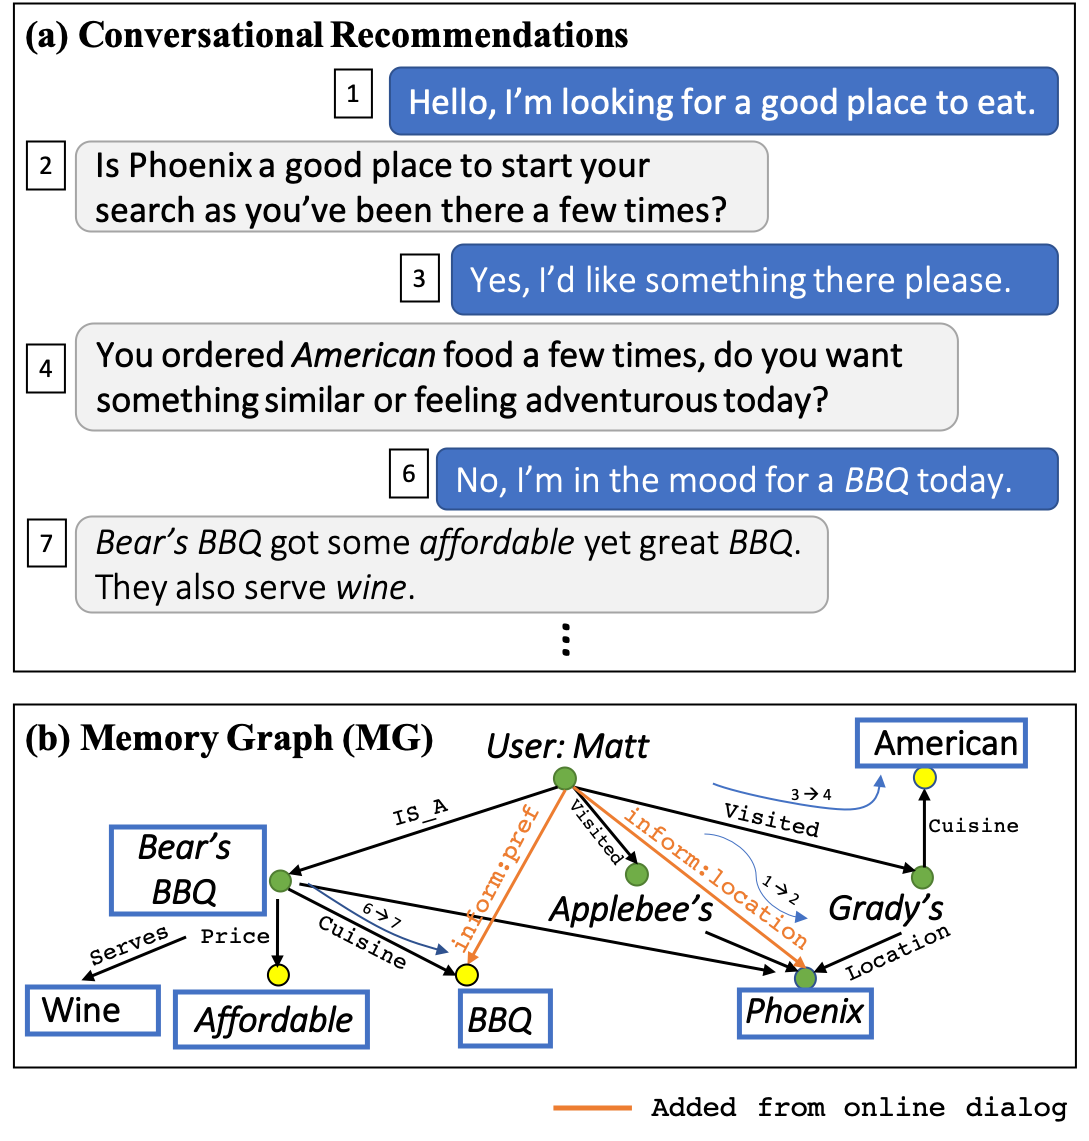
\includegraphics[width=0.9\columnwidth]{fig/acl19_teaser.png}
    \caption{A conceptual illustration of \textbf{Memory-grounded conversational recommendation}. (1) Conversational recommendation allows users to express preferences and requirements through dialogues. (2) Our \textit{MGConvRex} corpus is grounded on the memory graph (MG), which represents user's past preferences as well as newly added preferences.}
\label{fig:dialogue}
\vspace{-3mm}
\end{figure}

Conversational recommendation systems \cite{li2018towards} are recently introduced to mitigate some of these challenges by tracking users' up-to-date preferences through dialogues.
Most of the previous works focus on extending the conventional task-oriented dialogue literature with a recommender system, which allows the conversational system to update user preferences online by asking relevant questions (called ``System Ask User Respond (SAUR)'' for the current dialogue.

In summary, existing systems either favor a static offline recommendation over existing users or items or obtain short-term online updates on users' preferences via dialogues.
However, they unnaturally contrast offline with online preference learning and neglect the fact that the knowledge about a user is \textit{cumulative} in nature.
An intelligent system should be able to dynamically maintain and utilize knowledge about a user collected so far for recommendations.

To this end, we first introduce a novel concept called \textit{user memory graph} to represent dynamic knowledge about users and associated items in a structured graph (e.g., previous offline history of items visited/recommended, user preferences newly obtained through dialogues, etc.), allowing for easy and holistic reasoning for recommendations.
We then propose a new conversational recommendation system grounded onto this graph, conceptually defined more formally as follows:

\noindent\textbf{Memory-grounded Conversational Recommendation}:
Given the history of previous items $\mathcal{H}$ (interacted or visited, etc.), candidate items $\mathcal{C}$ for recommendation, and their attributes (values), 
an agent first (1) constructs a user memory graph $\mathcal{G} = \{(e, r, e')\vert e, e' \in \mathcal{E}, r \in \mathcal{R} \}$ for user $e_u$; 
then (2) for each turn $d \in D$ of a dialogue, the agent updates $\mathcal{G}$ with tuples of preference $\mathcal{G}' \gets \mathcal{G} \cup \{(e_u, r_1, e_1), \dots\}$ ;
(3) performs reasoning over $\mathcal{G}'$ to yield a dialogue policy $\pi$ that
either (i) performs more rounds of interaction by asking for more preference, 
or (ii) predicts optimal (or ground truth) items for recommendations $\mathcal{T} \subset \mathcal{C}$.

\textbf{Related Work}\\
\textbf{Conversational Recommendation}:
Much existing research on conversational recommendation focus on combining a recommender system with a dialogue state tracking system, through the ``System Ask User Respond (SAUR)'' paradigm.
Once enough user preference is collected, such systems often make personalized recommendations to the user.
For instance, \cite{li2018towards} proposes to mitigate cold-start users by learning users' preferences during conversations and by linking the learned preferences to existing similar users in a traditional recommender system.

\cite{sun2018conversational,kang2019recommendation} propose a reinforcement learning (RL) setting for a conversational recommendation system, where the dialogue policy is learned with multiple policies and recommendation signals.

\cite{zhang2018towards} leverages reviews to mimic online conversations to update an existing user's preference and re-rank items.

\noindent \textbf{Task-oriented Dialogue Systems} are widely studied with multiple popular benchmark datasets \cite{dstc2, woz, multiwoz, multiwoz2.1,sgd-dst}.
Most of the state-of-the-art approaches \cite{trade,bert-dst-alexa,bert-dst-cmu} focus on improving dialog state tracking with span-based pointer networks, which predicts information essential in completing a specified task (e.g., hotel booking, etc.)

Note that while conversational recommendation systems bears similarity to task-oriented dialogue systems, the key difference is that conversational recommendation aims to collect user's fine-grained soft preferences or sentiments, and utilize them collectively for ranking of items or asking better questions (policy selection), instead of collecting hard constraints (e.g., number of people, time and location) to filter a database and locate a record. 

\noindent \textbf{Graph Reasoning}:
Graph network \cite{scarselli2008graph,duvenaud2015convolutional,defferrard2016convolutional,kipf2016semi} is a type of neural networks proposed to operate on graph structures. 
A number of extensions to the original graph neural network have been proposed \cite{li2015gated,pham2017column},
most notably R-GCNs \cite{schlichtkrull2018modeling}, which can be applied on large-scale and highly multi-relational data.
Many applications of GNNs include \cite{Xian2019ReinforcementKG}, which introduces graph-based reasoning for an offline recommendation system.
A few works have recently been proposed to allow graph reasoning in dialogue systems.
\cite{Moon+19a, Moon+19b} propose new corpus to learn knowledge graph paths that connect dialogue turns.
\cite{tuan-etal-2019-dykgchat} introduces a knowledge-grounded dialogue generation task given a knowledge graph that is dynamically updated.
However, these workes often focus on response generation and do not address the conversational recommendation task.


\textbf{Preliminary on Semantic Space}\\
\label{chap6:sec:form}

As discussed in the introduction, one key step to enable a dialogue being grounded and maintained on a user memory graph is to first define the semantic space of dialogue acts, items, their slots and values (we borrow these terms from task-oriented dialogue system, which refer to items' attributes) for utterances from both the user and agent.
As a result, agents can turn unstructured utterances into structured data for user memory graph maintenance, integration and potentially future explainable reasoning for policy.
In this section, we first introduce the dialogue acts for recommendation and then introduce slots and values specifically defined for the recommendation in a restaurant domain.

\textbf{Dialogue Acts}
\label{chap6:sec:dialog_act}

The goal of designing dialogue acts $\mathcal{A}$ is to formalize the intentions from both the user and agent sides. 
Table \ref{chap6:tbl:dialog_act} demonstrates the dialogue acts for both the user and the agent.
From the agent's perspective, 
note that although existing conversational recommendation\cite{sun2018conversational,li2018towards,zhang2018towards} assumes a passive user interacts with the system and propose a System Ask – User Respond (SAUR) paradigm, we further allow the user to actively participate in the recommendation by allowing User Ask - System Respond (UASR) paradigm. In our dialogue act, \textit{Open question}, \textit{Yes/no question} and \textit{Inform} can be used by a user to actively participate in the conversation. The dataset we created from crowd workers also indicates that human likes to use these active dialogue acts in the context of conversational recommendation (see Appendix).


\begin{table*}
    \centering
    \scalebox{0.65}{
        \begin{tabular}{l|l l}
        \hline
        \textbf{Dialogue Act $a$} & \textbf{Description} & \textbf{Examples} \\
        \hline
        \textbf{User-side} & & \\
        \hline
        Greeting & Greeting to the agent & I'd like to find a place to eat. \\
        Inform & Actively inform the agent your preference & I'd like to find a \textit{thai} restaurant . \\
        Answer & Answer to a question from the agent & I prefer \textit{thai} food. \\
        Reply & Reply to a recommendation & I'll give it a try.\\
        Open question & Actively ask an open question about a recommended item. & What kind of food do they serve ? \\
        Yes/no question & Actively ask an yes/no question about a recommended item. & Do they serve \textit{thai} food ? \\
        Thanks & Thanks the agent & Thanks for your help. \\
        \hline
        \textbf{Agent-side} & & \\
        \hline
        Greeting & Greeting to the user. & How may I help you today ?\\
        Open question & Ask an open question about a slot to the user & What kind of food do you prefer ? \\
        Yes/no question & Ask a yes/no question about a value of a slot & I saw you've been to \textit{thai} restaurant, do you still like that ? \\
        Recommendation & Recommend items to the user. & How about \textit{burger king}, which serves \textit{fast food} ? \\
        Answer & Answers user's questions on an item. & They serve \textit{thai} food.\\
        Thanks & Thanks the user & Enjoy your meal. \\
        \hline
        \end{tabular}
    }
    \vspace{-2pt}
    \caption{Dialogue acts for agent and user $\mathcal{A}$: the spans of items/slot values are italized.}     
    \vspace{-11pt}
\label{chap6:tbl:dialog_act}
\end{table*}

\textbf{Slots and Values}
\label{chap6:sec:slotvalue}

This paper focuses on the recommendation in the restaurant domain.
We utilize the customer review dataset, which is widely used in existing research in recommender systems.
By leveraging the metadata of restaurants, we define slots $\mathcal{S}$ and their values $\mathcal{V}$ as shown in Table \ref{chap6:tbl:dialog_slot}. 
We select $\vert \mathcal{S} \vert = 10$ popular slots with rich values that can be encountered in the restaurant domain.
We omit the full set of values for brevity and only list a few examples. (Please refer to our dataset for the exhaustive list).

\begin{table}
    \centering
    \scalebox{0.7}{
        \begin{tabular}{l|l}
        \hline
        \textbf{Slot $e_s$} & \textbf{Example Value $e_v$} \\
        \hline
        location & Las Vegas, NV; Toronto, ON\\
        category & fast food; burger; thai\\
        price & cheap; expensive\\
        parking & garage; valet; lot\\
        noise & average; quiet\\
        ambience & classy; intimate\\
        alcohol & full bar; beer and wine \\
        good for meal & brunch; lunch; dinner\\
        wifi & paid; free\\
        attire & casual; formal\\
        \hline
        \end{tabular}
    }
    \vspace{-4pt}
    \caption{Available slots $\mathcal{S}$ and example of their associated values $\mathcal{V}$.}     
    \vspace{-10pt}
\label{chap6:tbl:dialog_slot}
\end{table}


\textbf{Dataset}\\
\label{chap6:sec:dataset}

Based on the definition in Section \ref{chap6:sec:form}, we create a large-scale dataset called \textit{MGConvRex}.
To the best of our knowledge, this is the first dataset for conversational recommendation that is grounded onto structured data of users' profile and items.
Although curating a dataset for a task-oriented dialogue system may involve building artificial scenarios (a pre-defined setting for collecting a dialogue) \cite{li2016user,li2018microsoft} due to limited access of real-world data for a particular task, conversational recommendation can leverage rich user behaviors that persist in the wild datasets of recommender system.  
As a result, we first introduce a simple way to create large-scale scenarios for dialogue transcription, as in Sec. \ref{chap6:sec:scenario}.
Then we set up a Wizard-of-Oz environment \cite{dstc2,woz,multiwoz,multiwoz2.1} to collect dialogues from crowd workers and further annotate transcribed dialogues based on scenarios, as in Sec. \ref{chap6:sec:woz}.
Our \textit{MGConvRex} can be used for research in almost all crucial components of a dialogue system such as natural language understanding, sentiment analysis, dialogue state tracking, dialogue policy generation, natural language generation, etc.

\textbf{Scenario Generation}\\
\label{chap6:sec:scenario}
A scenario is a pre-defined user-agent setting to collect a dialogue between two crowd workers, where one plays the user and the other plays the agent.
Let $\mathbb{B}=\{0, 1\}$ be a binary number.
We define a scenario consisting of the following parts: $(e_u, C, H, V, P, \mathcal{T} )$, where $e_u$ is a user, $C \in \mathbb{B}^{\vert \mathcal{C} \vert \times \vert \mathcal{V} \vert}$ means the candidate items $\mathcal{C}$ and their associated values $\mathcal{V}$, $H \in \mathbb{B}^{\vert \mathcal{H} \vert \times \vert \mathcal{V} \vert}$ is about visited items $\mathcal{H}$ and their values user $e_u$ has been to and known to the agent, $V \in \mathbb{B}^{\vert \mathcal{V} \vert \times \vert \mathcal{S} \vert}$ indicates values with their associated slots, $P \in \mathbb{B}^{\vert \mathcal{S} \vert \times \vert \mathcal{V} \vert} $ is the user preference (which value the user prefer for a slot) and $\mathcal{T} \subset \mathcal{C}$ is the ground-truth items. 
Each scenario is constructed in the following way:
\begin{itemize}
\setlength\itemsep{0.1em}
    \item Preprocess reviews to keep users and items (restaurants) with at least 10 reviews (10-core users/items). 
    We further filter out users with more than 100 reviews as they are suspected to be spam reviewers (not real-world users).
    \item Sort items (of reviews) by time and use a pre-defined timestamp (e.g.,  01/01/2014) to separate items into two groups: visited items and future items for all users.
    \item For each user, random select $\vert \mathcal{T} \vert = 1$ \footnote{We use 1 ground-truth item to reduce the load of the transcribers and increase the difficulty of reasoning.} items (with 4 or 5 ratings) as the \textit{ground-truth items} $\mathcal{T}$. Use the slots / values of the ground-truth items as \textit{user preference} $P$.
    \item For each user, negatively sample $\vert \mathcal{C} \vert - \vert \mathcal{T} \vert $ items and combine them with the ground-truth items $\mathcal{T}$ as \textit{candidate items} $\mathcal{C}$ \footnote{We choose $\vert \mathcal{C} \vert \in [10, 20]$ candidate items.} from all available items\footnote{To allow real-world recommendation setting, we ensure certain similarity over candidate items such as all locations are from the same state as the ground-truth items.}.
    \item For each user $e_u$, create two scenarios: one with \textit{visited items} $\mathcal{H}$ and one without. We keep $\vert \mathcal{H} \vert \in [5, 20]$ visited items to ensure enough statistical information for a user's past history.
\end{itemize}

\begin{table*}
    \centering
    \scalebox{0.83}{
        \begin{tabular}{l|c|c|c||c|c|c|c}
        \hline
        \textbf{Dataset} & \multicolumn{3}{c||}{\textbf{All Dialogues}} &  \multicolumn{2}{c|}{\textbf{Dialogues w/ History }} & \multicolumn{2}{c}{\textbf{Dialogues w/o History}} \\
        \hline
         & \# of Dial. & \# of Turns & Avg. \# of Turns & \# of Dial. & Avg. \# of Turns & \# of Dial. & Avg. \# of Turns \\
        \hline
Train & 3225 & 30858 & 9.57 & 1570 & 9.52 & 1655 & 9.62 \\
Dev & 266 & 2488 & 9.35 & 137 & 9.18 & 129 & 9.53 \\
Test & 2078 & 19818 & 9.54 & 982 & 9.45 & 1096 & 9.61 \\
        \hline
        \end{tabular}
    }
    \caption{\textbf{Statistics of the Dataset}: Dialogs w/ or w/o History indicates whether scenarios include visited items $\mathcal{H}$. }     
\label{chap6:tbl:dataset}
\end{table*}

\textbf{Wizard-of-Oz Collection}\\
\label{chap6:sec:woz}
We build a wizard-of-oz system to randomly pair two crowd workers to engage in a chat session, where each scenario is split into two parts:
$(P, \mathcal{T})$ for user and $(e_u, C, H, V)$ for the agent.
So in each session, the worker playing the user can see a user's preference $P$ and ground-truth items $\mathcal{T}$. 
The worker playing the agent can only see candidate items $C$ and the user's visited items $H$ (if a scenario contains that).
The user can tell the agent information from preference $P$ via utterance or check whether recommended items $e_i \in \mathcal{T}$ and reply to agent accordingly (they are not allowed to tell the ground-truth directly). 
The job of a worker playing the agent is trying to guess the ground-truth item $e_t \in \mathcal{T}$, based on the values of the available candidate items $C$, the current preference collected from the user via dialogue, and optionally the user's visited items $H$.
As a result, the goal of a conversation is like a game between the user and the agent, where the agent needs to guess the user's current preference and find the ground-truth item.
The collected behavior from the agent side reflects human-level intelligence of reasoning over candidate items for recommendation.
After transcribing a dialogue, we further ask the workers to rate the whole dialogue and each other's work, where
dialogues with ratings lower than 4 are filtered out.
Lastly, we annotate dialogue acts, items, slots, values and users' utterance-level and entity-level sentiment for each turn of dialogues.
The guidelines, screenshots of the Wizard-of-Oz UI can be found in the Appendix.

\noindent \textbf{Summary of \textbf{MGConvRex}}:
\label{sec:dataset_stat}
After annotation, we split the dialogues by their associated scenarios into training, development and test sets.
Note that we enforce all sets to have no overlapping on users so that the training cannot carry the knowledge from any particular user into testing.
The statistics of MGConvRex can be seen in Table \ref{chap6:tbl:dataset}.

\textbf{Results}\\
\label{chap6:sec:exp}

\textbf{Experimental Framework}\\
While there exist many frameworks for task-oriented dialogue systems \cite{li2016user,li2018microsoft,lee2019convlab} due to its popularity,
to the best of our knowledge, there's no existing framework for conversational recommendation.
Hence we first develop a new framework  \footnote{We will release the code along with baselines for future research.} for training, offline and online evaluation of supervised (imitation) learning and reinforcement learning agents.
One key component of our framework is the rule-based user simulator, which can be served for both evaluation and training of reinforcement learning agent\footnote{The the user simulator is detailed in Appendix.}.

\textbf{Evaluation Metrics}\\
We propose the following metrics to evaluate UMGR over the MGConvRex dataset both offline (against the collected dialogues) and online (against user simulator).

\textbf{Offline metrics}\\
We report the following metrics to evaluate the model's performance on dialog acts prediction, turn-level prediction over entities (items, slots, and values), and dialogue-level item prediction.

\noindent \textbf{Act Accuracy \& F1} are reported for all dialog acts against turns in the testing set.

\noindent \textbf{Entity Matching Rate (EMR, k@1, 3, 5)} (Turn-level): these metrics measure the predicted top-$k$ entities against the annotated test dialogues. 
Note that the types of predicted entities (items, slots or values) depend on the predicted dialogue acts $\hat{y}^\mathcal{A}$, so correctly predicted entities must have correctly predicted dialogue acts first.

\noindent \textbf{Item Matching Rate (IMR)} (Dialog-level): this measures all predicted items in a dialogue against the ground-truth item $e_t$.

\textbf{Online metrics}\\
In addition to offline evaluation, we report the following online metric against the user simulator to dynamically test the performance of recommendation. This mitigates an assumption in offline metrics that all past turns (from the human-annotated dialogues) are correct, which limits the interactive evaluation of conversations.

\noindent \textbf{Success Rate}: tracks whether the interaction with user simulators yields the ground-truth item $e_t$. We use the scenarios from the same test-set dialogues used for the offline evaluation. The maximum number of turns is simulated as 11.

\begin{table*}[!t]
    \centering
    \scalebox{0.83}{
        \begin{tabular}{l|l|l|l|l|l|l||c}
        \hline
\multirow{3}{*}{\textbf{Methods}} & \multicolumn{6}{c||}{\textbf{Offline Evaluation}} & \multicolumn{1}{c}{\textbf{Online Evaluation}} \\
\hline
& \textbf{Act Acc.}  & \textbf{Act F1} & \multicolumn{3}{c|}{\textbf{EMR}} & 
\textbf{IMR} & \textbf{Success Rate} \\
\hline
& & & @1 & @3 & @5 &  & \\
\hline
\hline
RandomAgent & 0.1769 & 0.182 & 0.0229 & 0.0229 & 0.0229 & 0.052 & 0.0659 \\
RecAgent      & 0.2568 & 0.0681 & 0.0262 & 0.0262 & 0.0262 & 0.3826 & 0.3855 \\
Pretrained Emb. & 0.2859 & 0.0741 & 0.1264 & 0.2484 & 0.316 & 0.0 & 0.0 \\
%UMGR & 0.61 & 0.5 & 0.22 & 0.38 & 0.44 & 0.33 & &  \\
\hline
%UMGR & Act Acc.  & Act F1 & \multicolumn{3}{c|}{EMR @1 @3 @5} & IMR & SuccessRate \\
\hline
UMGR (Proposed) & \textbf{0.643} & \textbf{0.5534} & 0.2329 & \textbf{0.4416} & \textbf{0.487} & 0.5226 & \textbf{0.4315} \\
- No Dialogue Acts & 0.3914 & 0.2137 & 0.2503 & 0.4383 & 0.4777 & 0.6165 & 0.4293 \\
- Prev. User Act Only & 0.6187 & 0.5375 & 0.2255 & 0.4175 & 0.4561 & 0.5693 & 0.4032 \\
- Static $\mathcal{G}$ & 0.6355 & 0.5452 & 0.0957 & 0.2769 & 0.3494 & 0.0914 & 0.11 \\
\hline
%UMGR on w/ or w/o His. & Act Acc.  & Act F1 & \multicolumn{3}{c|}{EMR @1 @3 @5} &  IMR & SuccessRate \\
\hline
UMGR w/ History & 0.5778 & 0.4761 & 0.0769 & 0.2111 & 0.2987 & 0.2872 & 0.2592 \\
UMGR w/o History & 0.6146 & 0.4575 & 0.0597 & 0.1546 & 0.2498 & 0.1122 & 0.1032 \\
        \hline
        \end{tabular}
    }
    \vspace{-2pt}
    \caption{Results of both offline and online evaluation: EMR stands for entity matching rate, which compares all types of predicted entities against annotated ones when the dialogue act is predicted correctly; IMR stands for item matching rate, which evaluates predicted items against the ground-truth item across all turns.}     
    \vspace{-12pt}
\label{chap6:tbl:result}
\end{table*}

\textbf{Compared Methods}\\
Our framework implements the following methods:\\
\noindent \textbf{RandomAgent}: As a baseline, we implement an agent that randomly picks a dialogue act and randomly pick a candidate item/slot/value to fill the current response to the user.\\
\noindent \textbf{RecAgent}: The agent always chooses \textit{Recommendation} as the dialog act to enact and select a random item that has not been tried from candidate items. This leads to sub-optimal performance as it does not use or collect user preferences.\\
\noindent \textbf{Pretrained Embeddings}: 
We pre-train the graph embeddings for all entities and relations from the MG across all scenarios in the training set using the TransE-based graph prediction approaches \cite{Nickel+15}.
We utilize these for prediction of the future item/slot/value without having the R-GCN layers.
While this approach is widely used in the related literature and carries cross-scenario knowledge, we show that using pre-trained graph embedding alone is sub-optimal for a particular user and that the dialogue policy needs to perform dynamic reasoning over the user memory graph.\\
\noindent \textbf{UMGR} (\textbf{Proposed}): This is the proposed R-GCN based model. We choose the batch size to be 32, all hidden states to be size 64. The number of maximum dialogue acts is set to 10. We use 5 layers of R-GCN based on validation on the development set. $\alpha, \beta, \gamma$ are set as 10, 10, 100 based on the scales of losses of different types, respectively. 
% \todo{check missing hyperparameters} 
We further conduct the following ablation studies.\\
\noindent \textbf{- No Dialog Acts}: this study removes the dialogue acts encoder, demonstrating the importance of the dialogue acts in policy generation.

\noindent \textbf{- Prev. User Act Only}: this study only uses the most recent dialogue act from the user. We use this to show how many past dialogue acts are needed for good policy generation.

\noindent \textbf{- Static $\mathcal{G}$}: uses the initial user memory graph without making any updates during the conversation. We use this study to demonstrate that dynamic update of the user memory graph is crucial for reasoning better dialogue policy.\\

\noindent \textbf{- w/ History} v.s. \textbf{- w/o History}: analyzes the effect of the history of visited items $\mathcal{H}$ (the last two dataset folds in Table \ref{chap6:tbl:dataset}). We use these two baselines to demonstrate that prior knowledge of user memory history aids in predicting dialogue policy.


\textbf{Results}\\
The results are shown in Table \ref{chap6:tbl:result}. From the results, we can see that UMGR achieves good performance for most of the metrics.
%\todo{we didn't talk about a rule-based agent I think it's fine. agreed} 

\noindent \textbf{UMGR} is effective in leveraging knowledge in the user memory graph.
While the UMGR model already achieves reasonable accuracy in dialogue policy prediction relying just on the user memory graph (\textit{-No Dialogue Acts}),
adding previous dialogue act from the user (\textit{- Prev. User Act Only}) significantly improves the performance.
%The competitive performance with (\textit{- Prev. User Act Only}) indicates that a good amount of user knowledge is contained in the user memory graph, without having to resort much to previous turns.
Lastly, we show that keeping user memory graph updated is crucial, as seen in \textit{static $\mathcal{G}$} not providing good rankings for entities.  

\noindent \textbf{UMGR vs. Pre-trained Graph Embeddings}. We confirm that the static pre-trained graph embeddings provide limited capacity for reasoning over a large-graph across multiple scenarios to learn user-specific dialogue policy, leading to poor performance in the recommendation.

\noindent \textbf{w/ \textit{vs} w/o Hisory}. Lastly, the contrasting results for with and without visited items $\mathcal{H}$ in a user memory graph indicate that having more knowledge about a user's past experience is important in conversational recommendation.

\textbf{Conclusion}:
We build a conversational recommendation system that can collect and maintain a user's up-to-date needs and preferences for the recommendation.
We release a novel dataset with \textit{user memory graph} grounding based on scenarios generated from the behaviors of real-world users.
The user memory graph has the benefits of both accumulating pieces of knowledge about a user and interpretability.
Experimental results on our R-GCN based reasoning model (UMGR) show promising results for dialogue acts, items, slots and values prediction.


\appendices
\newpage
\appendix

\bibformb
\bibliography{BibFile}

\newpage
% \vita
% This is where the vita goes.  Its organization is left as an exercise.
\clearpage
\pagestyle{pageontop}
\thispagestyle{pageonbottom}
%\vspace*{3in}
\begin{large}
\begin{center}
{\bfseries VITA}
\end{center}
\end{large}
\begin{tabular}{p{2.8cm}p{10.5cm}}
NAME: & Hu Xu  \\ 
    &\\
EDUCATION:  &Ph.D., Computer Science, University of Illinois at Chicago, Chicago, Illinois, 2020. \\  
            &\\
            &M.Eng., Electronics and Communication Engineering, Peking University, Beijing, China, 2009.\\
            &\\
%            &B.Eng., Computer Engineering, University of Illinois at Chicago, Chicago, Illinois, 20xx.  \\
            &\\
ACADEMIC EXPERIENCE:  &Research Assistant, Big Data and Social Computing Lab, Department of Computer Science, University of Illinois at Chicago, 2015 - 2020. \\
            &\\
			&Research Assistant, Social Media and Data Mining Lab, Department of Computer Science, University of Illinois at Chicago, 2017 - 2020. \\
			&\\
            &Teaching Assistant, Department of Computer Science, University of Illinois at Chicago: \\
            &\squishlist            
            \item Language and Automata, Fall 2015, Spring/Summer/Fall 2016 and Fall 2017.    
            \item Compiler Design, Spring 2017 
            \squishend \\

 \end{tabular}

\end{document}
